
\ifx\isEmbedded\undefined

\documentclass[12pt,a4paper]{report}
\usepackage[bottom=2.5cm,left=2.0in,right=2.5cm]{geometry}

% FONT RELATED
\usepackage{times} %Move to times font
\usepackage[labelfont=bf,textfont=it]{caption}

% LINKS, PAGE OF CONTENT, REF AND CROSS-REF, HEADERS/FOOTERS
\usepackage{footmisc}
\usepackage{hyperref}
\usepackage{bookmark}
\usepackage{fancyhdr}
%\usepackage{nameref}

% FIGURES, GRAPHICS, TABLES
\usepackage{graphicx}
\usepackage{parskip}
\usepackage{tocloft}
\usepackage{array}
\renewcommand{\cftfigfont}{Figure }
\renewcommand{\cfttabfont}{Table }
\usepackage{longtable}

%\newlength{\mylen}
%\renewcommand{\cftfigpresnum}{\figurename\enspace}
%\renewcommand{\cftfigaftersnum}{:}
%\settowidth{\mylen}{\cftfigpresnum\cftfigaftersnum}
%\addtolength{\cftfignumwidth}{\mylen}






%\usepackage{subfigure}
\usepackage{wrapfig}
\usepackage{caption}
\usepackage{subcaption}


% COLOURS, TEXT AND FORMATTING
%\usepackage[left=2.0in,right=0.5in]{geometry}

\usepackage{array}
\usepackage{color}
\usepackage{setspace}
\usepackage{longtable}
\usepackage{multirow}


% ADVANCED MATHS, PSEUDO-CODE
\usepackage{amsmath}
\usepackage{amsfonts}
\usepackage{alltt}
%\usepackage{algorithm2e}
\usepackage{algorithmicx}
\usepackage{algorithm}
\usepackage{algpascal}
\usepackage{algc}
\usepackage{algcompatible}
\usepackage{algpseudocode}
\usepackage{linegoal}

% BIBLIOGRAPHY
\usepackage{natbib}
%\usepackage[authoryear]{natbib}
%\usepackage{harvardnat}
\bibpunct{(}{)}{;}{a}{}{,}
%\usepackage{bibentry}
%\nobibliography*



% LINE NUMBERS
%\usepackage{lineno}
%\linenumbers

% USE IN DISSERTATION:

% MARGINS
%\setlength{\oddsidemargin}{2.0in}
%\setlength{\evensidemargin}{0.5in}
%\setlength\headsep{2.5in}

% TEXT
\setlength\textheight{9.5in}
\setlength\textwidth{5.1in}

% indent at each new paragraph
\setlength\parindent{1.0cm}
%\setlength\parindent{0.5cm}

%\setlength{\parskip}{10.5ex}

\setlength\topmargin{-0.2in}

% 1.5 spacing:
\renewcommand{\baselinestretch}{1.5}
%\renewcommand{\baselinestretch}{1.3}
%\fontsize{15}{15}\selectfont

% USE IN REPORT:

%\setlength\oddsidemargin{1cm}
%\setlength\evensidemargin{0.3in}
%%\setlength\headsep{2.5in}
%
\setlength\textheight{9.0in}
%\setlength\textwidth{5.5in}
%
%% indent at each new paragrapg
%\setlength\parindent{0.5cm}
%
%%\setlength{\parskip}{10.5ex}
%
%\setlength\topmargin{-0.2in}

%\newcommand{\HRule}{\rule{\linewidth}{0.5mm}}
\newcommand{\HRule}{\rule{\linewidth}{0.0mm}}

% Color definitions (RGB model)
\definecolor{color-comment}{rgb}{0.1, 0.4, 0.1}
\definecolor{color-variable}{rgb}{0.000,0.000,0.616}
\definecolor{color-question}{rgb}{0.4, 0.0, 0.0}
\definecolor{color-new}{rgb}{0.2, 0.4, 0.8}

\newcommand*{\Let}[2]{\State #1 $\gets$
\parbox[t]{\linegoal}{#2\strut}}

\newcommand*{\LongState}[1]{\State
\parbox[t]{\linegoal}{#1\strut}}

\graphicspath{{../images/}}
\begin{document}
%\maketitle
\fi




%**************************************************************************
%**************************************************************************
\chapter{Cloth Modelling and Re-targeting }
\label{cha:cloth_retargeting}

This chapter presents an automatic pattern based cloth modelling method that generates fit cloth for characters. Based on character measurements acquired by the method presented in chapter.\ref{cha:geodesic}, the shape of cloth patterns are automatically adjusted. This method is able to create fit cloth efficiently for different characters with different body shapes and proportions without tedious manual operation that is required in traditional pattern based cloth modelling methods. 


%**************************************************************************
\section{Introduction}

In computer animation, creating assets such as models or scenes for a film is time consuming and costly. Therefore, the reusability of assets is curial to the film production budget. For rigid model such as cars or buildings, once created, they are stored into a asset warehouse and can be used in other films with little tweaking required. Such assets can also be traded among animation studios or animation artists. However, for clothes, their shapes follow the profile of a character, in most cases, they are bespoken for a particular character. Usually, constructing a complete set of outfits for an animation character takes a well trained animation artist several days to finish. Due to the large difference between character designs among different films, reusing cloth models requires a large amount of manual operation to fit a cloth to another character with different body shapes and proportions.

Cloth is a soft object whose shape is determined by its design, body shape and posture of the wearer. Same cloth dressed by different character will results different cloth shapes. Moreover, in computer animation, characters are usually modelled in different postures, it is difficult to define a unified 3D form for cloth model to be stored, distributed and reused because for every different character, 3D cloth model needs to be heavily modified in order to cope with the new  character body shapes and proportions. 

In fashion industry, after generations of development, cloth pattern has become an important medium that transfers cloth design into wearable object. Cloth patterns are the basic items that constitutes a functional cloth. In order to implement a cloth design, firstly, the design needs to be broken down into a set of textile pieces, then through the assembling techniques such as stitch and adhesive, pieces are assembled together in a predetermined order to form a complete cloth. The process that breaks down a cloth design into patterns is called ``patternmaking'' \Citep{armstrong2000}. Through this process, cloth design is transferred from design concept into a set of patterns that can be cut from the raw textile material. Therefore, the same cloth design can be reproduced easily\Citep{Millard:1919}. Modern cloth pattern is designed to follow the measurements of standard body template to maximize the generality. Then, by providing the measurements of a specific customer, the shape of each pattern can be adjusted respectively to fit the customer. In massive cloth production, a complex pattern resizing procedure named is developed to adapt the needs for dressing general public. Cloth pattern grading aims at resizing the cloth into several size categories based on the human anthropometric statistic data to fit the most individuals in the general public\Citep{moore2001concepts}. 

Cloth pattern in fashion industry has provided a standard to preserve a cloth design, when utilising made-to-measure tailing technique, it can be resized to fit any customer. The cloth modelling method presented in this chapter adapts this custom tailoring techniques from fashion industry into computation animation. The basic idea is that, clothes are stored in the form of cloth patterns, when modelling cloth for a character, the measurements are acquired for pattern shape adjustment. Each pattern is adjusted based on the corresponding measurements from the character. Finally, cloth pattern are assembled together following a predefined sewing rule to form a complete 3D cloth. .


However, in virtual world, the body shapes and proportions of a animation character are only limited by the imagination of artists, therefore, using size chart developed from real human body to perform proportional scaling to fit cloth to a animation character with exaggerated body shape longer applies. Therefore, for each unique character, their cloth needs to be bespoken from measurements. However, resizing cloth pattern based on measurements requires deep tailoring knowledge which few animation artist process, the difficulty of properly resizing a set of cloth pattern has become bottle neck for the application of pattern based cloth modelling method in computer animation. In order to improve the reusability of clothes in computer animation production, this chapter presents an automatic cloth pattern resizing method to adjust cloth pattern based on the measurements of a character. By automating the cloth pattern resizing process, deep knowledges in tailoring are no longer required in this method. Clothes model can be stored in an unified form (cloth pattern) into asset warehouse, with the presented automatic pattern resizing method, by providing measurements of a new character, cloth pattern can be reused to dress a different character with different body shapes and proportions. Figure \ref{figure:workflow} demonstrates the general workflow of the pattern based cloth modelling method presented in this chapter

 \begin{figure}[H]
    \centering
	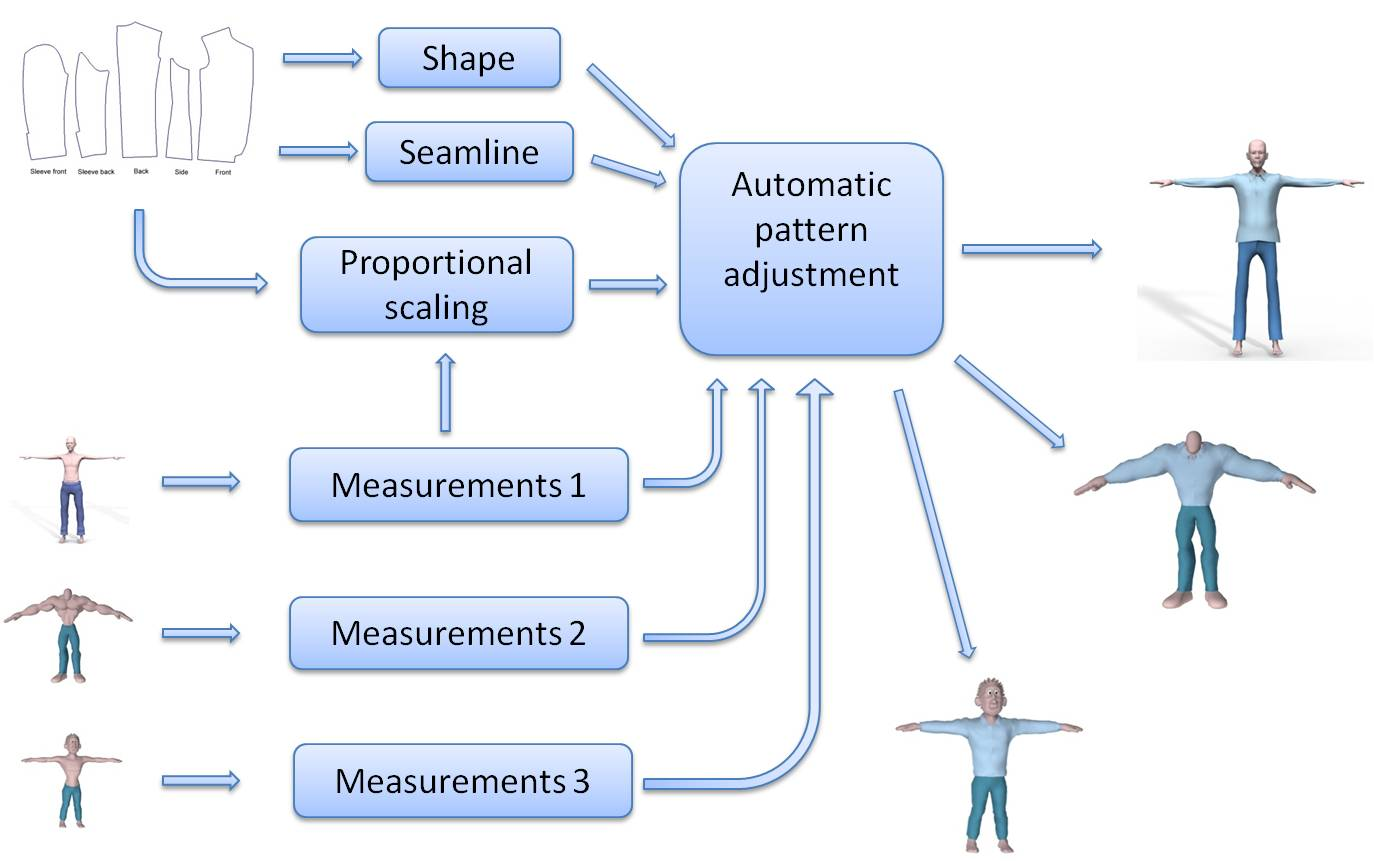
\includegraphics[width=1\columnwidth]{../images/general_workflow}\\[1cm]
    \caption{Workflow of pattern based cloth modelling method presented in this thesis}
    \label{figure:workflow}
\end{figure} 


%
%Normally, modelling a cloth from cloth patterns involves three steps, firstly, the 2D cloth patterns have to be created, then patterns are placed onto the 3D character model, finally, physical simulation is performed to stitch all the patterns together. If the cloth needs to be adjusted, the modifications are carried out on 2D cloth patterns and this entire process needs to be performed iteratively till the cloth fits to the character. Moreover, if the same cloth design needs to be dressed onto a different character who has different body shapes and proportions, this tedious process would needs to be repeated again from scratch. To make matter worse, adjusting cloth pattern to fit to a character requires lots of tailoring expertises, few animation artist possess such knowledge. Therefore, current pattern based cloth modelling methods are rarely used in the production of the films or games.

%When using geometrical modelling method to create cloth, that is, to model cloth patch by patch(polygon, nurbs or subdivision). This approach seems easier than pattern based modelling technique because the cloth can be modelled directly onto the character and the appearance of the cloth can be viewed throughout the modelling process, therefore the fit of the cloth is guaranteed. However, this advantage only exists when modelling cloth for one character, the geometrical modelling method also suffers from the same drawback as the pattern based cloth modelling method when handling multiple characters. That is the modelling process needs to be repeated from scratch to fit a cloth onto different characters with different body shapes and proportions. 

%Followed by the fast development of computer hardware and computer graphic techniques, more and more characters can be handled simultaneously. However, limited by current cloth modelling techniques, dressing different characters with different body shapes and proportions is still considered as a very tedious and time consuming process. 

%In computer animation, cloth for each character needs to be modelled individually in order to fit their unique body shapes and proportions. The tediousness and unintuitiveness of the current pattern based cloth modelling methods are getting worse when dressing multiple different characters with different body shapes and proportions. However, many methods such as \Citet{brouet:hal-00695903, Achim2002} were developed for dressing different characters automatically, their methods fit a cloth to a new character by adjusting 3D cloth mesh directly. The resulting cloth patterns are extracted after the cloth adjustment by using 3D surface flattening techniques. Despite the extra computation required by this method, the pattern shape distortion introduced by 3D surface flattening process can not be avoided. Therefore, the preservation of the cloth pattern can be hardly maintained. 


%**************************************************************************
\subsection{Patternmaking}

\Citet{armstrong2000} defines cloth patterns as the templates from which parts of a garment are traced onto the fabric before cutting out and assembled. When creating patterns, blocks(also as known as slopers) are created first. Blocks are two-dimensional templates that consists of basic design of the a cloth type\Citep{Howland2008}, Figure \ref{figure:BlocktoPattern} demonstrates a block for suit. Blocks are constructed based on the measurements taken from standard body template or the wearer\Citep{armstrong2000}. When measurements are taken from an individual, it provides a good indication of the body dimension that a cloth design is intend to fit. In made-to-measure tailoring, measurements acquisition is particularly important since it directly determines the fit of cloth. Therefore, this process is usually performed by an experienced tailor. In massive cloth production, blocks are usually created by using measurements from a size chart which is based on a particular ethnic or group of the target customers. For example, US standard clothing size chart\Citep{USsizeChart2010} contains body proportions of the general public of the Americans and European standard clothing size chart\Citep{UKsizeChart2005} contains the size data of the people who were born in Europe. Based on the blocks, cloth patterns are created by introducing pockets, style line, drapes and other adjustments. Figure \ref{figure:garmentBlock} demonstrate the blocks for a woman's shirt.
 
\begin{figure}[H]
	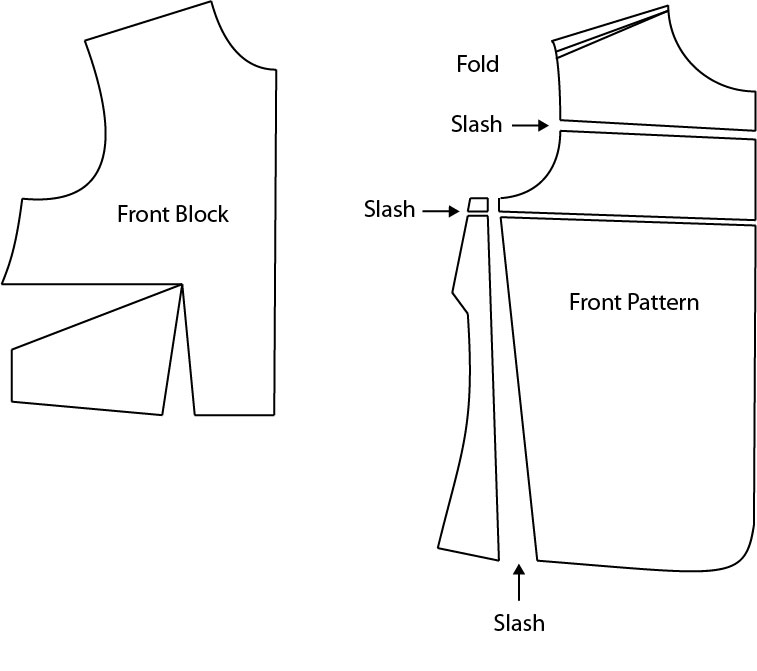
\includegraphics[width=\columnwidth]{../images/block_pattern}\\[0.1cm]
    \caption{Block(left) and a pattern(right) made from it by adding details\Citep{Howland2008}.}
    \label{figure:BlocktoPattern}
\end{figure}

\begin{figure}[H]
	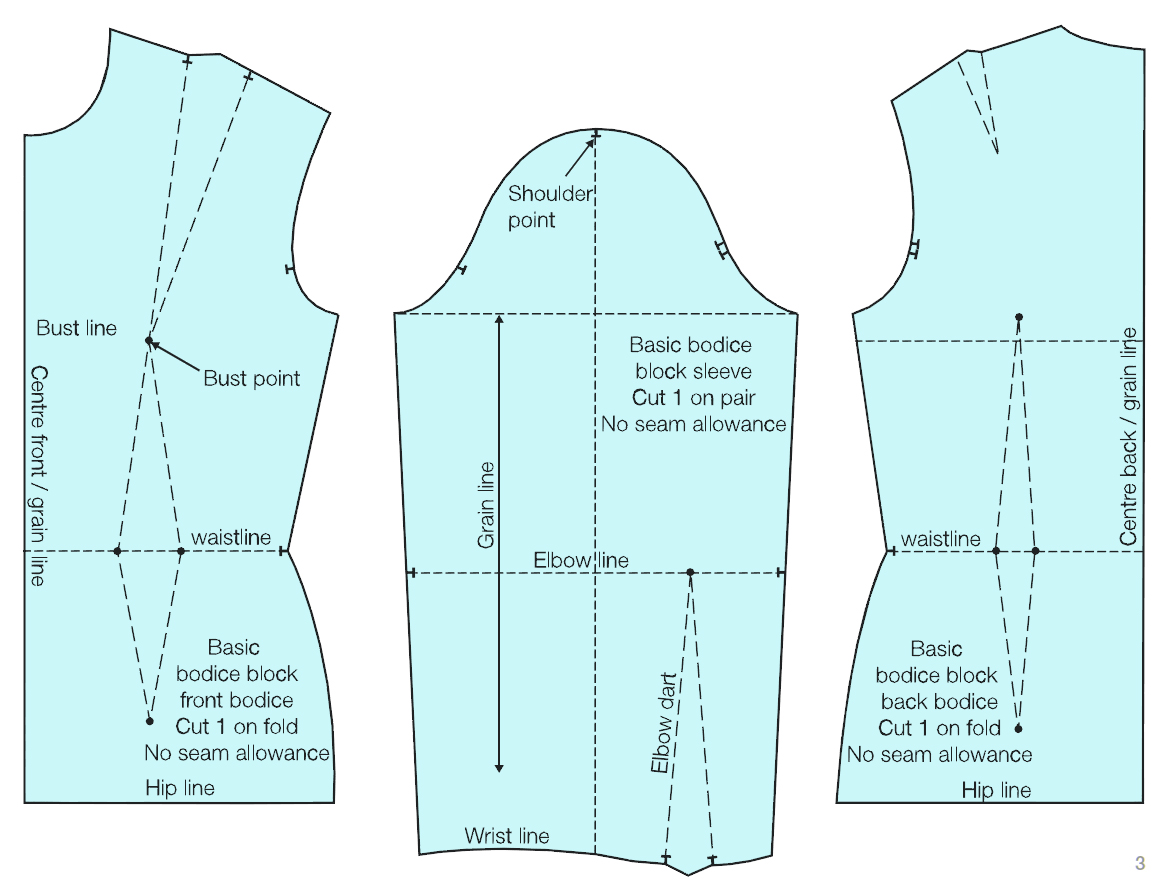
\includegraphics[width=\columnwidth]{../images/garment_block}\\[0.1cm]
    \caption{Garment blocks for woman shirt\Citep{rosen2004patternmaking}.}
    \label{figure:garmentBlock}
\end{figure}

Figure \ref{figure:garmentBlock} demonstrates landmarks that are associated with datum points on a character on a set of blocks. Pattern grading is the process of systematically increasing and decreasing dimensions of patterns in to a range of sizes for production. During pattern grading, patterns are scaled proportionally into different sizes with predefined intervals introduced by a size chart. This process not only retains the original design of the cloth during distribution but is also very cost effective during the process of manufacturing due to the people who fit a predefined size are normally distributed into an interval introduced by a size chart \Citep{Schofield01012005,moore2001concepts}. 

However, in computer animation the situation is much more complexer than in reality. In reality, for each ethic or certain group of people, the similarity of body proportion exists among individuals. In virtual world, the body proportion is only limited by the imagination of artists, therefore using size chart to perform proportional scaling to patterns to create fit cloth no longer applies to the virtual character. In most cases, clothes for animation character are bespoken to a particular character. Reusing a cloth to another character with different body shapes and proportions requires large amount of modification.


\subsection{Pattern Resizing Criteria}

During pattern grading process, all patterns are scaled proportionally to preserve the shape of pattern respectively \Citep{moore2001concepts}. However, as aforementioned, the body proportion of the virtual character is significantly different from humans. Therefore, performing proportional scaling to patterns might leads to an undesired result.  

\begin{figure}[H]
	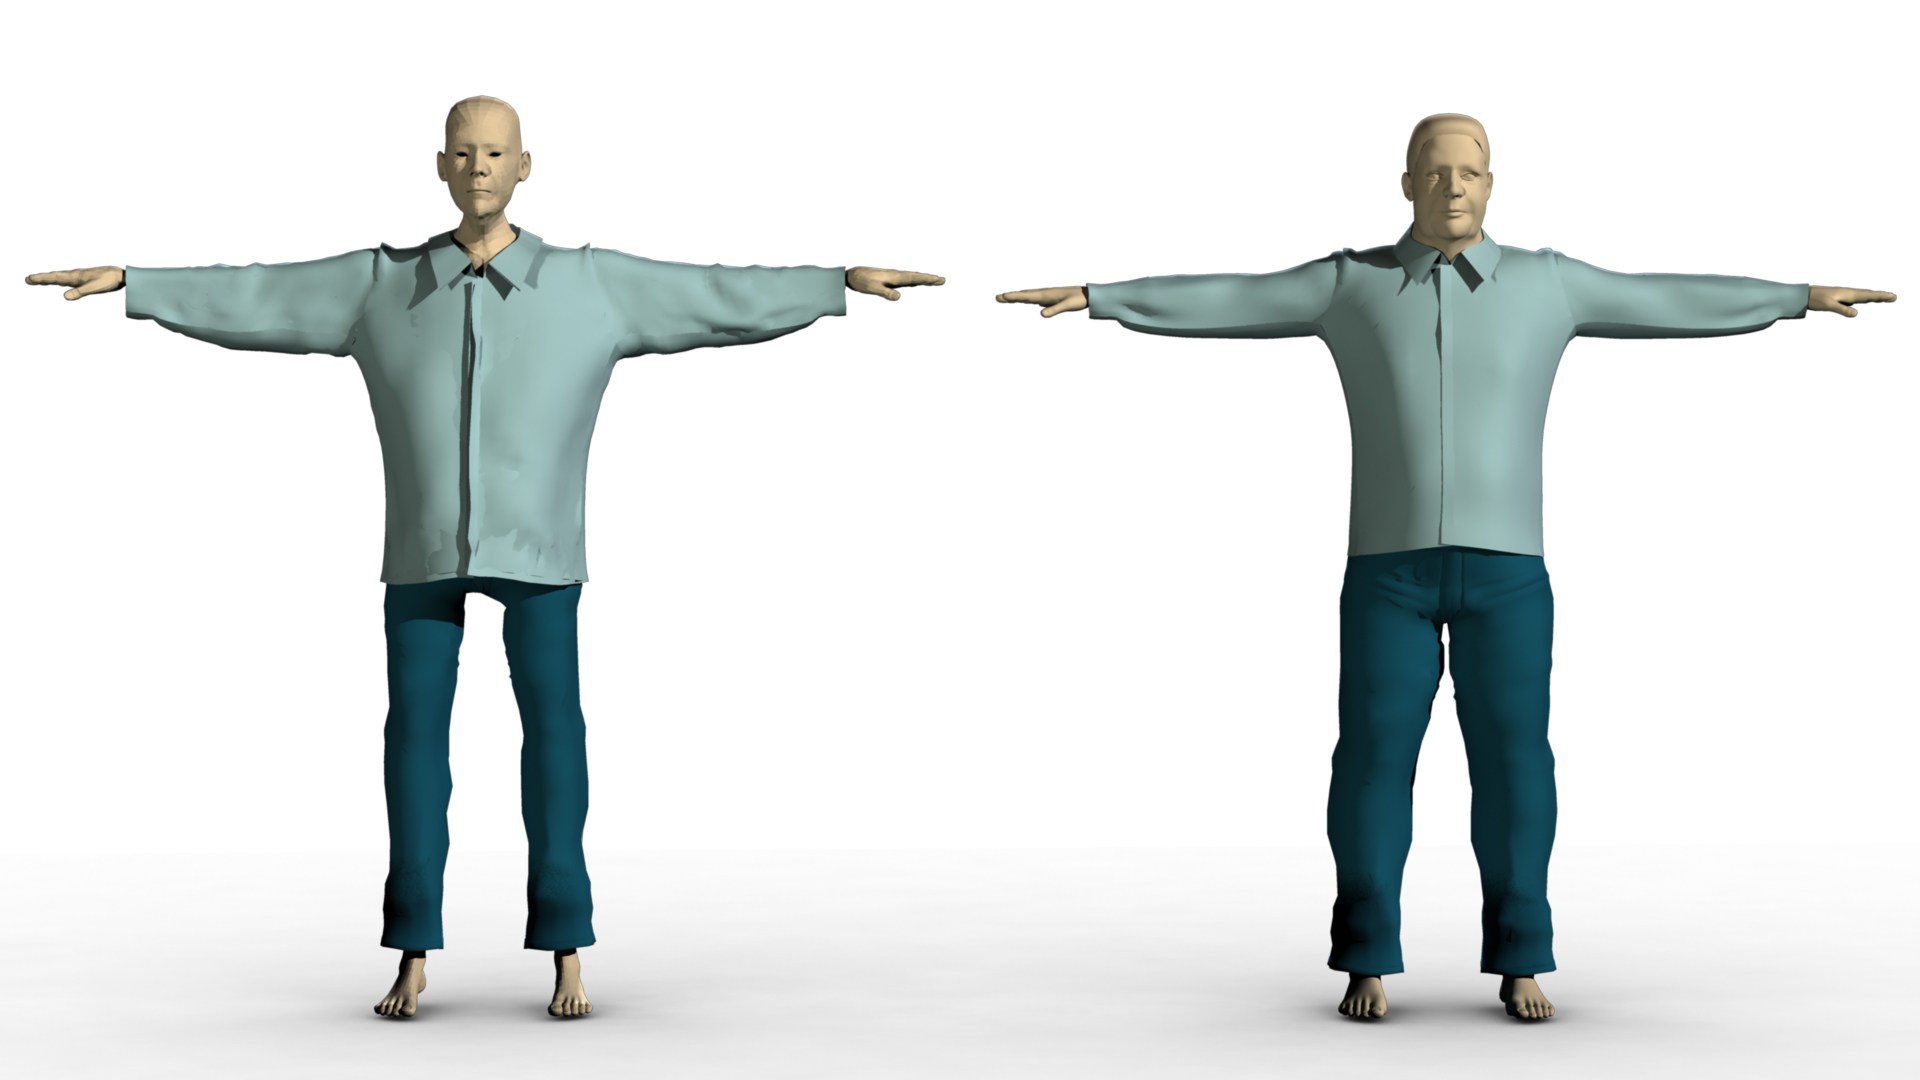
\includegraphics[width=\columnwidth]{../images/sknny_fatty}\\[0.1cm]
    \caption[Same shirt on different characters]{Same shirt proportional scaled to different characters with same arm span and height using method presented by \Citet{moore2001concepts}}
    \label{figure:fs_compare}
\end{figure}

Figure \ref{figure:fs_compare} demonstrates the result of using same shirt to dress two characters with same height and arm span using proportional scaling method presented by \Citet{moore2001concepts}. Because these two characters share same height with is the major measurements used to define the interval of a size chart, both of the character falls into the same grading intervals. Therefore, clothes are adjusted into same size. However, the character on the right is much stronger than the one on the left, the body of right side character supports cloth much better than the other. On the contrary, the skinny character has much thinner limbs which results a baggy shirt. In order to achieve better fit, during made-to-measure cloth tailoring, extra measurements such as ``Arm Hole Length'' or ``Cuff Girth'' are taken from customer in order to fine tune the cloth for better fit. With those extra measurements, different parts of a pattern are scaled in different manners. In order to generate patterns based on the measurements, a few geometric criteria need to be evaluated in order to ensure the fit of cloth as well as maintaining the design of cloth. 

\begin{description}
\item[Character Measurements] 
Cloth pattern represents different parts of a garment, which responsible for covering certain parts of body, therefore, all the patterns need to be deformed in a manner that each pattern matches to the measurements of its corresponding body part. Because all the patterns are derived from blocks, during pattern adjustment, for each block which a pattern is developed from, the distance between  landmarks that are associated with the datum points on the character body needs to satisfy  the requirement set by the measurements taken from the character. Especially when the character has an unusual body proportion, different parts of a block might be scaled in different fashions. For instance, in Figure \ref{figure:fs_compare}, the arm of both two characters have the same length, however, the circumference of arm are mush different, Moreover, despite the difference between the circumference of arms, the wrist girth are the same for both characters. Therefore, in order to satisfy the all the measurement requirements, different parts of sleeve pattern need to be adjusted in different manners.

\item[Pattern shape] 
Cloth pattern is the most basic component of a complete garment and the shape of each pattern defines the shape of cloth. Pattern grading process is considered as the most difficult process during the tailoring which only the professionals is able to master. The overall shape of a cloth pattern can be altered significantly to accommodate the difference of body proportions between different customers. However, details of the pattern such as slops, darts and their relative location are kept \Citep{moore2001concepts}. In computer animation, the goal of transferring cloth from one character to another is to fit a cloth onto a different character without altering the design of the cloth. However, each cloth pattern needs to be adjusted independently in order to match the measurements from character. Therefore a shape evaluation process is needed after adjusting cloth pattern in order to maintain the design of the cloth. 


\item[Seam Line] 
In reality, cloth patterns need to be stitched together to form a complete garment. The adjacent edges between two patterns is the seam-line. A seam-line consists of many pairs of stitching points which are located on the boundary of two adjacent patterns. During the adjustment of pattern, each pattern is adjusted individually to meet the measurements. Therefore there is no guarantee that after the adjustment of the patterns, the seam-line remains consistent. Because seam-line determines the location of the patterns after it is assembled into a complete garment, without the preservation of the seam-line, original design of the cloth cannot be preserved.

\end{description}

%**************************************************************************

\section{Cloth Resizing Algorithm }
In this section, an automatic cloth pattern adjusting method is presented. This method operates cloth size adjustment directly on 2D patterns and optimizes each pattern to ensure all the patterns satisfy the criteria introduced in previous section.

Two inputs are required for this method. The first input is a group of patterns representing a cloth design. Within each pattern, the landmarks that associated with the datum point on character body are defined.  Pattern landmarks are key points on a pattern inherited from block. They are defined on the cloth block by patternmaker to associate body measurements with the length on a block \Citep{rosen2004patternmaking}. In real world, pattern landmarks are used as a guide line for pattern resizing where tailor adjusts distance between pattern landmarks to meet body measurements. Moreover, seam-lines are presented along with the pattern. Figure \ref{figure:pattern_example} demonstrates an example of input patterns.

\begin{figure}[h]
	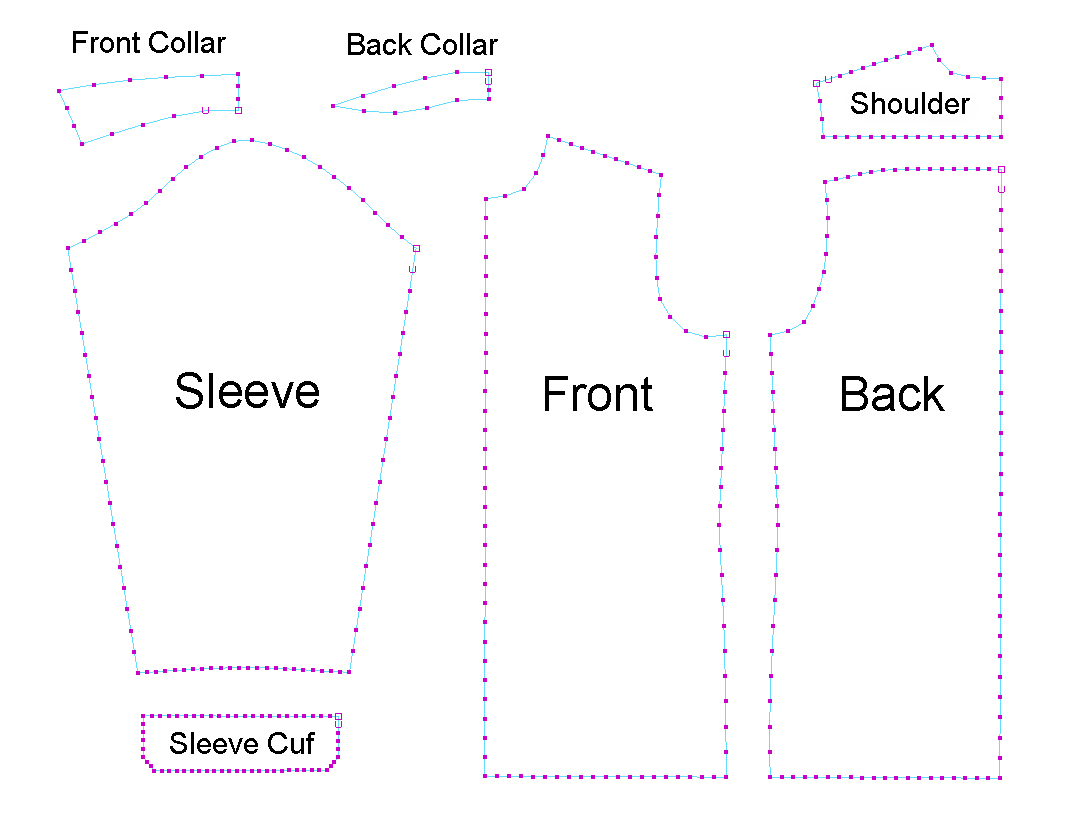
\includegraphics[width=\columnwidth]{../images/pattern_example}\\[0.1cm]
    \caption{An example of a cloth pattern}
    \label{figure:pattern_example}
\end{figure}

The second input is the 3D character model which is modelled in a ``T-pose''. Because this method involves physical simulation for pattern assembling process, the contact between limbs will leads to the penetration between cloth mesh and character skin. Moreover, the measurements of the character are also provided by using the method from previous chapter.

In order to properly determine the size of patterns, block for each pattern is generated at first. In fashion industry, cloth pattern is created from an unique block by adding details. Therefore, in this method, a block is refers to a 2D bounding box of each pattern and all the landmarks that are associated with datum points on character body are defined on the blocks. Moreover, because a block and a pattern have a strictly one to one association which means for any pattern, it is generated from only one unique block. Also, because a block contains much less details than the pattern, performing pattern adjusting algorithm on blocks can saves lots of computational resources.

When constructing a block from a pattern, firstly, the ``critical points'' on a pattern are selected. The ``critical points'' are defined by points which are the most capable of representing the geometrical features of a pattern. For example, the sharp turning points on the contour of the pattern or extreme points are considered as ``critical points''. Figure \ref{figure:block_example} illustrates ``critical points'' on the sleeve pattern. Finally, a bounding box is created for each pattern, within the bounding box, for every ``critical point'', two orthogonal line are created to form a grid. This is demonstrated in Figure \ref{figure:block_example}. 

\begin{figure}[h]
	\centering
	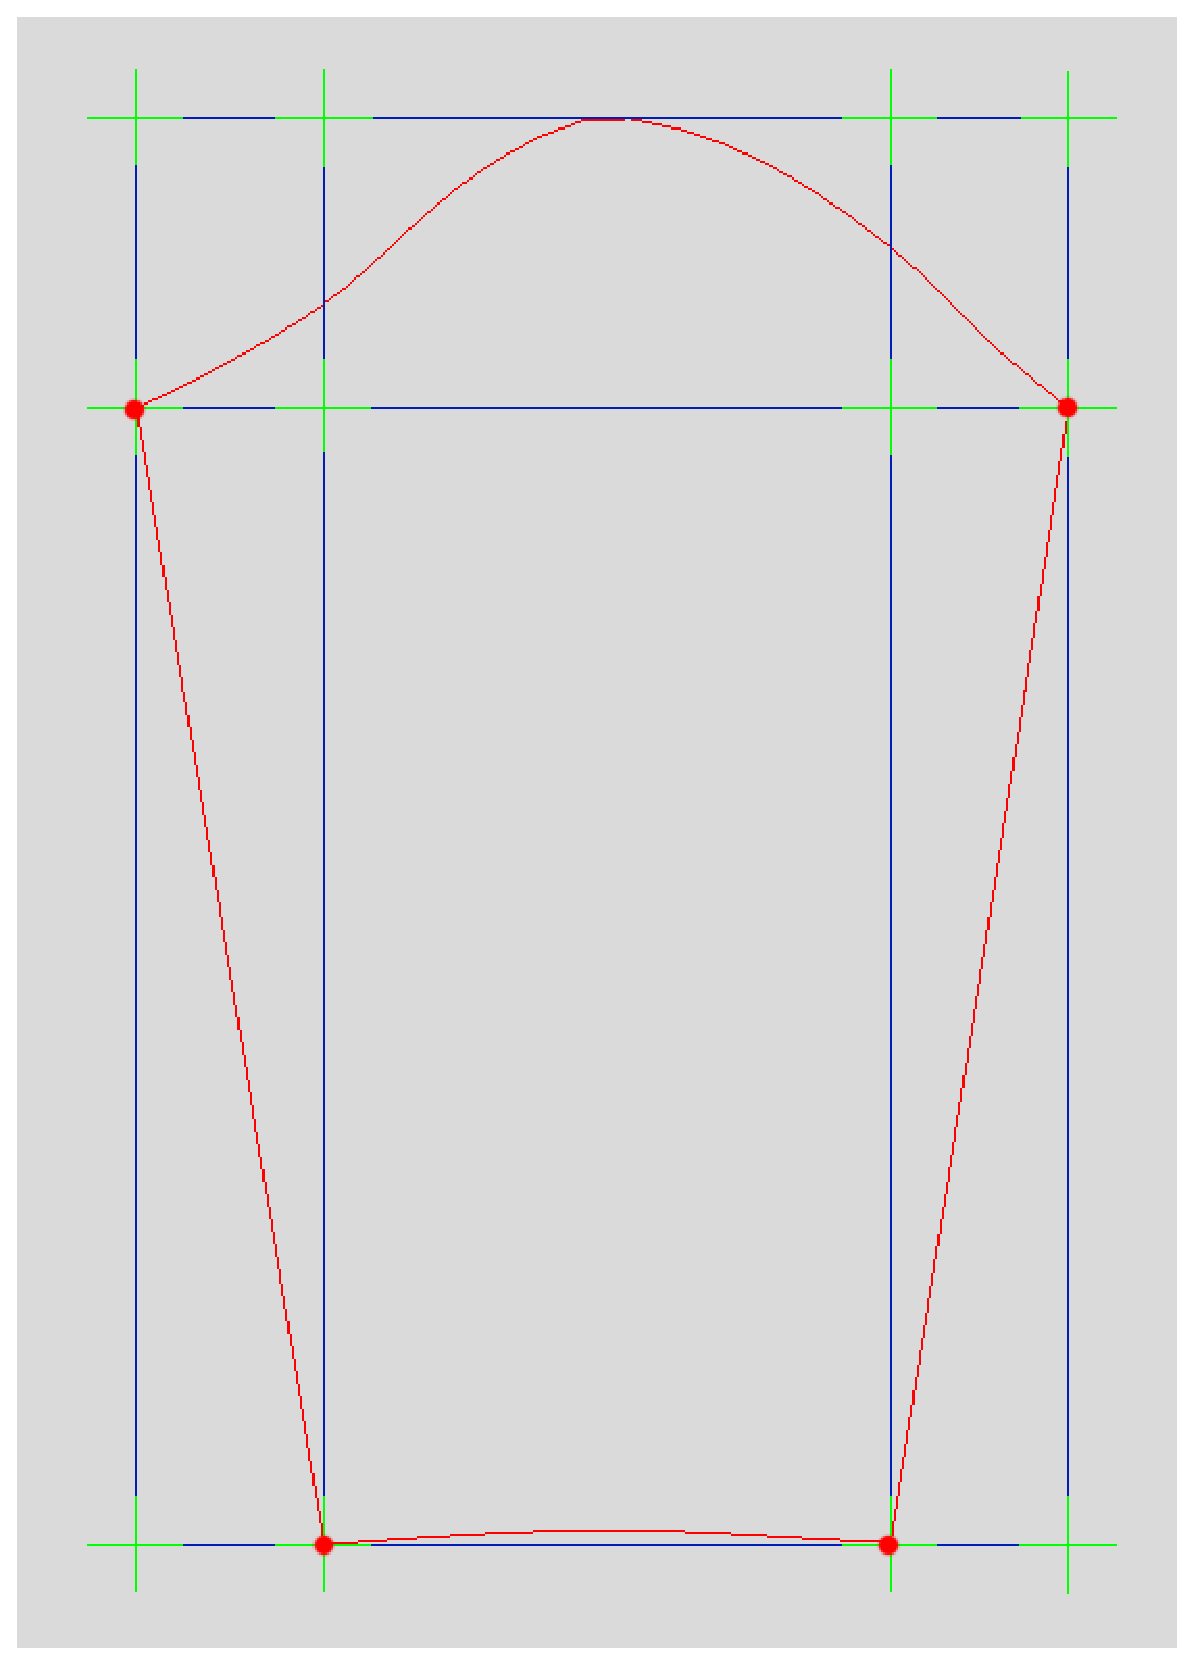
\includegraphics[width=0.5\columnwidth]{../images/block}\\[0.1cm]
    \caption[Pattern and its block]{Block generated for sleeve pattern(red closed curve). The red points are ``critical points'' on sleeve pattern.}
    \label{figure:block_example}
\end{figure}

Next, based on the gird, a nurbs plane is constructed and control points of the nurbs plane are intersection points on the grid( this is demonstrated by the green cross in Figure \ref{figure:block_example} ). All points on each pattern can be represented by a parametric coordinate on the nurbs plane. For every pattern, a unique nurbs plane is created and it is considered as the block of the given pattern. 

Then, the proportional scaling used in traditional cloth grading method is performed onto each pattern. In general, the measurements that are associated with the length of limbs are used as the reference for scaling such as ``Back Length'' for torso patterns and ``Arm Length'' for sleeve patterns. Figure \ref{figure:block_proportional} demonstrates the result of performing proportional scaling to sleeve block based on the ``Arm Length'' measurement.  

\begin{figure}[h]
	\centering
	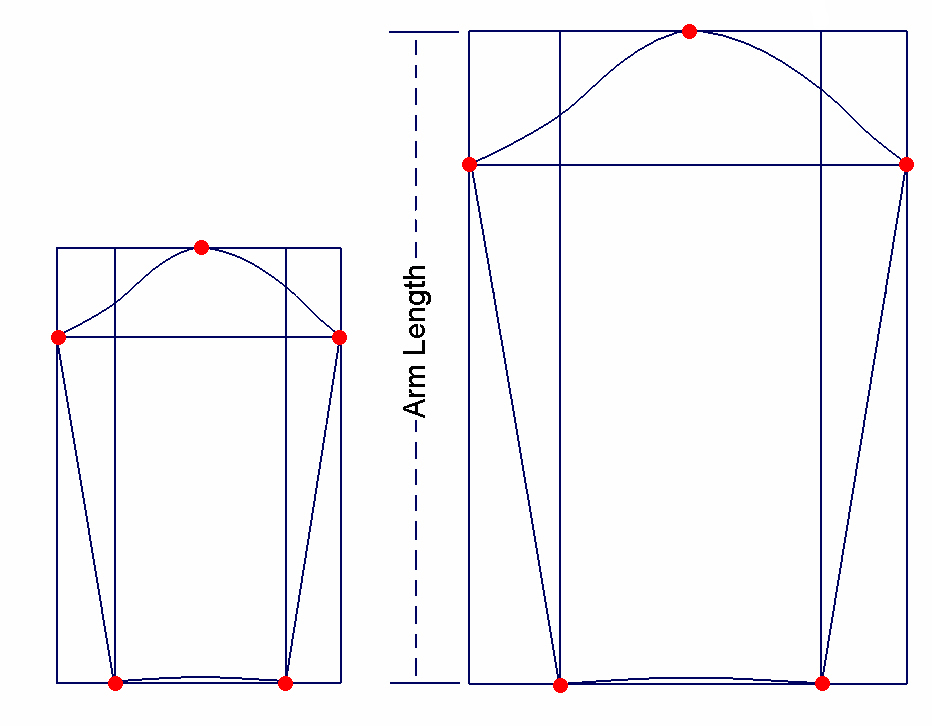
\includegraphics[width=0.7\columnwidth]{../images/block_proportional_scaling}\\[0.1cm]
    \caption[Blocks before and after the proportional scaling]{Block before(left) and after(right) the proportional scaling. The height of the sleeve pattern after scaling has reached the measurement ``Arm Length''}
    \label{figure:block_proportional}
\end{figure}


\begin{figure}[H]
	\centering
	\includegraphics[width=0.9\columnwidth]{../images/all_block_proportional_scaling}\\[0.1cm]
    \caption{Blocks after proportional scaling is performed.}
    \label{figure:all_block_proportional}
\end{figure}

%The proportional scaling of the patterns a significant drawback that needs to be improved. Firstly, in order to perform the proportional scaling, at least one measurement must be provided as scaler. However, for some patterns, such as ``collar'', it does not have a measurement that is directly associated with. Therefore the proportional scaling can not be performed onto such type of cloth pattern. As depicted in Figure \ref{figure:all_block_proportional}, ``Collar Front'' and ``Collar Back'' do not associate with any measurement taken from the character, Therefore, they cannot be resized by the proportional scaling method. Moreover, for such type of patterns, their size usually depend on the patterns that they are stitched to. For example, the ``Collar Front'' is stitch to ``Front'' and  ``Collar Back'' is stitched to ``Shoulder'', therefore, the size of ``Collar Front'' is depends on the size of ``Front'' and the size of ``Collar Back'' is depends on the size of ``Shoulder''.

Performing proportional scaling to cloth patterns has a significant drawback that needs to be improved. This drawback is demonstrated in Figure \ref{figure:confict}. 

\begin{figure}[H]
	\centering
	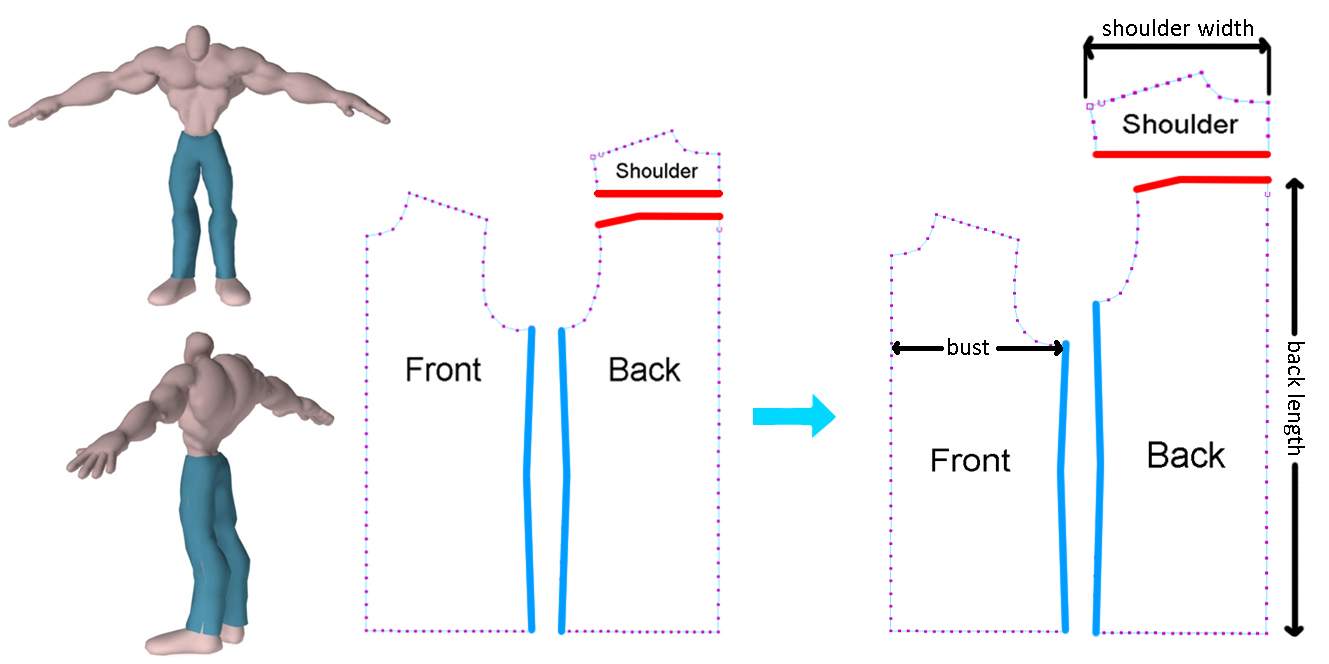
\includegraphics[width=1\columnwidth]{../images/confict}\\[0.1cm]
    \caption{Inconsistency of seam-line after scaled patterns proportionally}
    \label{figure:confict}
\end{figure}

Where `Front'', ``Back'' and ``Shoulder'' are three patterns of a cloth for Character A. Patterns are scaled according to their major measurement, For example, pattern ``Front'' is proportionally scaled based on measurement ``bust'', pattern ``Back'' is proportionally scaled based on measurement ``Back length''. However, when pattern was initially designed, each pair of seam-lines between two adjacent patterns usually have same length and interval for each stitch, this is shown in Figure \ref{figure:confict} as a pair of blue curves indicates a pare of seam-lines between pattern ``Front'' and ``Back'', a pair of red curves indicates seam-lines between pattern ``Shoulder'' and ``Back''. However, after proportional scaling is performed, the length of seam-line is no longer the same which further leads to undesired wrinkles around seam-line during pattern assembling process.  At this stage, each pattern has good fit on measurements criteria but worsen on the seam-line criteria. If patterns are adjusted to meet the seam-line criteria, the fit on measurements will be break. Moreover, if patterns are firstly proportional resized based on measurements and then adjusted each pair of seam-line to satisfy seam-line criteria, the shape of patter will be changed. Actually, in many cases, these conditions may not concord with each other and in some cases even conflict to each other. Therefore, it is very difficult to adjust cloth patterns to fit a character based on one criteria.   


\subsection{Genetic Algorithm}

Modelling a cloth from cloth patterns for a character requires each pattern to be adjusted individually. During the pattern adjustment, three criteria need to be satisfied in order to fit the cloth to the character as well as preserve the design and integrity of cloth. The goal of cloth fitting process is to generate a set of cloth patterns that constitute a complete garment which fits character while having the least distortion compare to original design of this garment. In this thesis, this process is considered as a multiple objective optimization process. 

Optimization problem is a very hot research area that has been studied intensively for decades and many techniques have been developed to tackle such a problem. In the case of cloth pattern adjustment, since a complete cloth is comprised by a set of patterns, each pattern is formed by a set of points (sampling points on the contour of a pattern). The parameters of this optimization problem are the coordination of these sampling points. 

%Furthermore, the size of the cloth need to be adjusted to meet the size of the character in order to generate fit cloth for virtual character. For pattern based cloth modelling methods, The size of each pattern is the key factor that depends the fit of the cloth. Current pattern based cloth modelling method generally adjust the cloth after patterns are assembled together. The fitting process is performed directly on the 3D cloth surface. The patterns for the fitted cloth are extracted after the adjustment has been performed on 3D cloth surface. 3D surface flattening techniques are used to extract 2D cloth pattern from 3D cloth surface. Not only this type of cloth modelling method requires extra step for the 2D pattern extraction, but also during the 3D surface flattening, distortion of the pattern could be introduced. 
%
%The cloth resizing method presented in this thesis directly operates on 2D cloth patterns. By using the tailoring techniques and patternmaking techniques in fashion industry, each 2D cloth pattern is adjusted based on its corresponding character measurements in order to generate cloth that fits the character. However, a complete cloth is a system that consisted by a group of patterns. When adjust the shape and size of each pattern accordingly, the maintenance of the interrelation between patterns is critical to the preservatives of the cloth design. Therefore, the cloth resizing process is a global optimization process that looking for the best combination of the shape and size of each pattern that both fits the character while maintain the original cloth design. 

For current gradient based optimization methods, handling large amount of parameters requires a lot of computational resources. Among many optimization methods, genetic algorithm dwarfs others by its simplicity and efficiency. Genetic algorithm works on chromosomes, which are encoded parameters of solutions. Because this encoding mechanism largely reduces the number of parameters used for optimization, much less computation is required by genetic algorithm. Moreover, unlike traditional optimization method, which searches cost surface from a single point, genetic algorithm searches cost surface in a parallel manner, it is not only able to scan a large number of potential solutions very quickly, but also able to avoid local optimal solution effectively due to its parallel searching method. In general, the advantages of the genetic algorithm over other optimization method are,

\begin{enumerate}
	\item Genetic algorithm searches through a wide range of the cost surface simultaneously. Therefore it is able to deal with very complex cost surfaces and avoid local minimum.
	\item Genetic algorithm works on the chromosome instead of real parameters, therefore it is able to handle large number of parameters.
	\item The initial proposals do not effect the final solutions as bad solutions are discarded by selection at every evolution. Therefore, the genetic algorithm is not sensitive to the initial seeds. 
\end{enumerate}

In the thesis, three criteria are used for evaluating fit and style preservation during pattern adjustment process. However, these criteria are often conflict to each other. The optimization algorithm needs to be able to handle multiple objectives. Moreover, cloth patterns are represented by a set of nurbs curves which are controlled by a set of ``Critical Points''. Each ``Critical Point'' is a parameter to the optimization, large amount of parameters need to be handled at same time. Furthermore, the initial state of pattern is proportionally scaled based on each pattern's major measurements, to some non-exaggerated human like character, it will provides a good approximation that is close to the final fit cloth. However, for some largely exaggerated character such as character A in Figure \ref{figure:confict}, proportional scaling will worsen other criteria. Therefore, cloth pattern optimization should not be sensitive to its initial seeds. Genetic Algorithm has advantages these three aspects, therefore, this thesis utilises genetic algorithm for cloth adjusting process. Because cloth patterns are adjusted based on the measurements of the character, adjusting cloth patterns using genetic algorithm has three extra benefits. Firstly, once the parameters are set, genetic algorithm evolve the initial seeds towards best solution automatically, therefore, given measurements of any character, this method can generates cloth patterns that fit the character automatically. By automating the pattern adjustment process using genetic algorithm, traditional tailoring knowledge is no longer needed for this process, the duplication of effort required by traditional pattern based cloth modelling method can be eliminated and the efficiency for modelling cloth for different characters with different body shapes and proportion can be largely improved. Secondly, this method empowers the creativity of animation artists and amplifies their productivity by allowing them to use a large amount of existing cloth patterns in the fashion industry to create various clothes that fit different characters. Thirdly, because the 3D cloth is generated based on the adjusted patterns, the work flow of modelling cloth for the character is one direction. There is no turning back for extracting patterns from 3D cloth which is required by current cloth modelling method. Therefore, the shape distortion that is introduced by 3D surface flattening process can be avoid. 

Genetic algorithm(GA) is an optimization method which is based on the principles of natural selection \Citep{haupt2004practical,deb2001multi}. During natural selection, effected by environment, the biological traits of organism become more or less common in a population through generations of reproduction. A genetic algorithm allows a population that consists of many individuals to evolve under certain rules and to a state that minimizes the cost function \Citep{Holland:1992}. 

A genetic algorithm starts from a group of randomly generated solutions called ``initial population''. Within the initial population, each individual is a set of variables that represents a solution of the problem. By evaluating every individual using cost function, a ranking is assigned to the individual in terms of performance of cost function. Then, a selection method is applied to select a group of individuals to perform crossover and mutation operation. Finally, the convergence of current generation is evaluated. If current generation does not reach the minimum on the cost surface, this process loops back to step one, the algorithm is executed iteratively till the minimum cost is reached, this procedure is demonstrated in Figure \ref{figure:GA_SO}

\begin{figure}[H]
	\centering
	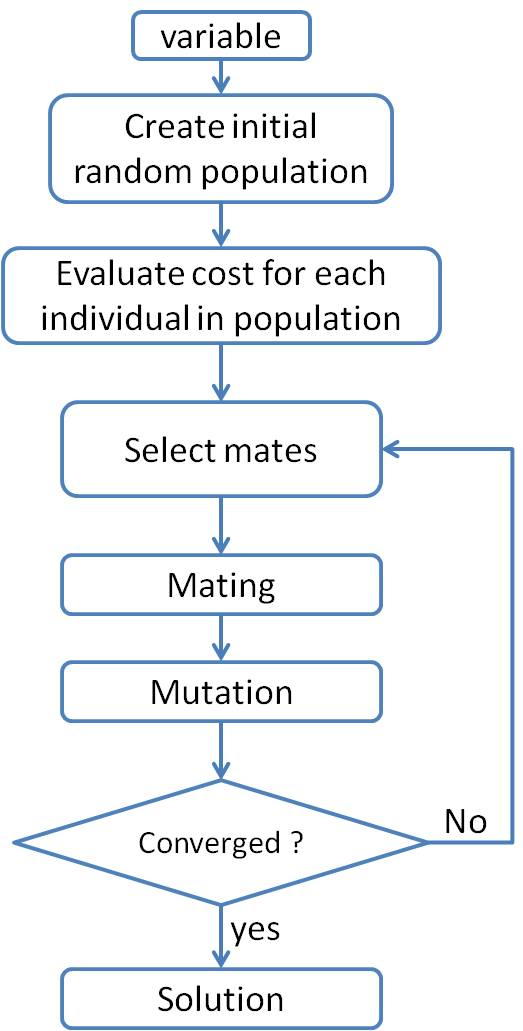
\includegraphics[width=0.5\columnwidth]{../images/GA_SO_flowchart}\\[0.1cm]
    \caption[Single objective genetic algorithm]{Workflow for single objective genetic algorithm}
    \label{figure:GA_SO}
\end{figure}

In genetic algorithm, ``fitness'' refers to the cost of an individual in terms of its performance to the cost function, higher the fitness, lower the cost. In single objective optimization, only one individual who has the highest fitness is selected as the final solution of the problem. However, in may applications, more than one objective are needed for describing the problem. Moreover, among these objectives, conflicts often occurs. For example, adjusting a pattern for a particular measurement usually leads to worsen the consistency of seam-lines. In this case, it is impossible to locate a single best solution that is optimum with respect to all objectives. This kind of optimization is called multi-objective optimization, the purpose of multi-objective optimization is to find as many good solutions as possible. The solution set results from a multi-objective optimization is called Pareto-optimal solutions \Citep{Pareto:1971}. However in may applications, only one solution is needed, therefore, usually, after Pareto-optimal solutions has been formed, a higher-level objective is used to select one solution out of the Pareto-optimal solutions as the final solution for the problem.

In the following section, a multi-objective genetic algorithm for pattern adjustment is presented in detail. This algorithm uses multi-objective optimization to find a combination of patterns that has best fits on measurement criteria, seam-line criteria and pattern shape criteria.

\subsection{Definition of Population}

Within a population, individual is the basic element represents one solution to the problem  \Citep{haupt2004practical}. In our case, each pattern is described by a set of points located on the contour of a pattern $Pattern_{i} = [p_{0}, p_{1}, ..., p_{n}] $. A block is a nurbs plane that the pattern is inscribed to and it is defined by a set of control points, noted as $b_{i} = [cp_{i1},... cp_{im}]$.  After a block is created based on a pattern, Points on the pattern can be interpolated by parametric coordinate on the block plane. Each pattern has its unique block, therefore, for each pattern, it can be represented uniquely by control points of the corresponding block plane. Note that $m << n$, which means the number of control points is much less than the actual number of points on the pattern, particularly, in experiments, $m$ ranging from 4 to 30 and $n$ ranging from hundreds to a thousand. Consequently, a pattern can be represented by control points of the block effectively. 

\begin{table}[H]
\centering
\begin{equation}
\left\{\begin{matrix}
b_{1}= & cp_{1_{1}} & cp_{1_{2}} & \cdots & cp_{1_{m}} \\ 
b_{i}= & cp_{i_{1}} & cp_{i_{2}} & \cdots & cp_{i_{m'}}\\ 
& &\vdots \\
b_{n}= & cp_{n_{1}} & cp_{n_{2}} & \cdots & cp_{n_{m''}}\
\end{matrix}\right.
\end{equation}

\caption{The structure of gene}
        \label{tab:chromosomes} % title of Table
\end{table}

Table \ref{tab:chromosomes} illustrates the structure of chromosomes. Where $cp_{i}$ denotes a control point on block $b_{i}$, an individual is comprised by a group of blocks $ind = {b_{1}, ... , b_{n}}$ which representing a complete cloth. In general, for each individual, a gene represents a control point, a chromosome represents a block, and an individual is constituted by a group of chromosomes (blocks).

The initial population is the first sample over the cost surface. Because in the case of pattern adjustment, the measurements of character can be largely different form character to character, the boundary of the cost surface can be difficult to determine. Although for GA, the initial population will not affects the formation of Pareto-front, setting the initial population close to the final objective can largely reduce the number of generations required for generating the Pareto-front. Therefore, before performing genetic algorithm, traditional proportional scaling method is used to initialize the first generation of population. For every input pattern, the measurements taken from the subject that associated with this pattern is stored into an array, denoted as $M_{i} = [m_{i_{1}}, ... , m_{i_{n}}]$. For each stored measurement, it contains datum points that this measurement is taken from and every datum point on the subject has an unique corresponding landmark on the pattern. This is illustrated in Figure \ref{figure:pattern_body_relation} 

\begin{figure}[H]
	\centering
	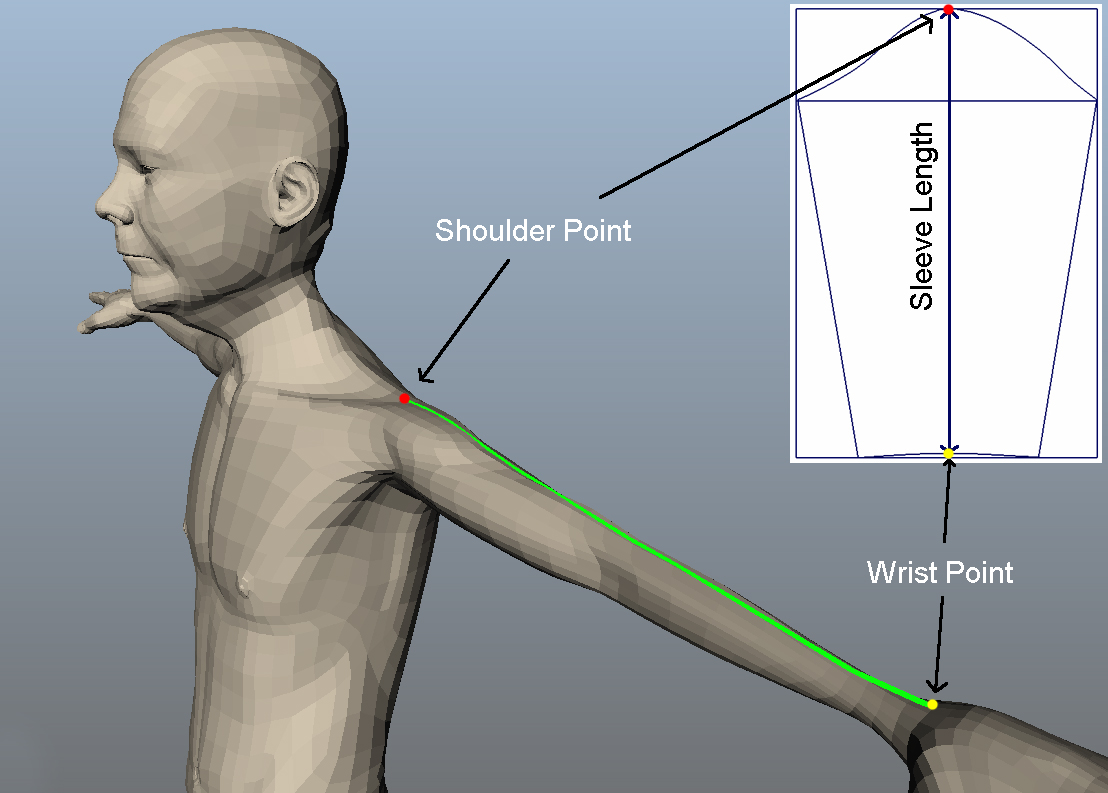
\includegraphics[width=1.0\columnwidth]{../images/body_pattern_mapping}\\[0.1cm]
    \caption[Association between body datum point and pattern landmarks]{Association between body datum point and patter landmarks. The green line is the geodesic from shoulder point(red point) to wrist point(yellow point). The red and yellow point on the sleeve pattern is the pattern landmarks that associated with the datum points on the body of character. When sleeve is well fitted, the ``Sleeve length'' should match the length of this geodesic.}
    \label{figure:pattern_body_relation}
\end{figure}

The scaling factor can be calculated by Algorithm \ref{algorithm:init_pattern}.

\begin{algorithm}
\caption{Initial Pattern}\label{algorithm:init_pattern}
\begin{algorithmic}[1]
\Procedure{Proportionally Scale Pattern}{Pattern $P$, Measurements $M$}
	\For{measurement $m_{i} \in M $}	
		\State $p_{s}$ and $p_{e}$ is two datum points of $m_{i}$ 
		\LongState{$l_{s}$ and $l_{e}$ is two landmarks on a pattern that $l_{s} \sim p_{s}$ and $l_{e} \sim p_{e}$}
		\State $d \gets$ distance between $l_{s}$ and $l_{e}$
		\State $Sr \gets m_{i} / d$($Sr$ denotes scaling factor)
	\EndFor
	\State Select largest $Sc$ from $S$ as the scaling factor for $P$
\EndProcedure
\end{algorithmic}
\end{algorithm}

By using $Sc$ as the scaling factor, the input patterns are proportionally scaled. Although the proportional scaling method cannot produce a well fit cloth for the character, it is able to resize the patterns to a certain degree so that the cloth roughly fits the character. Then, the proportional scaled patterns are used as the seed for generating the initial population. In the next step, in order to create individuals that spread over the cost surface, a mutation operation are carried out on each pattern to vary its shape. This operation will be explained in detail in ``Crossover and Mutation'' section.

In order to improve the efficiency of the evolution, the individual can age during the evolution. In nature, the size of the population changes over generations because individuals who carries a fit gene has better crossover opportunity than those who carries less fit gene. Therefore, naturally, a fit gene is able to live longer during evolution than a less fit genes. When a gene dies, the individual who carries this gene also dies. Consequently, the number of the individuals in a generation is determined by the death of the less fit gene. 

\begin{equation}
life_{i} = \left\{
\begin{matrix}
life_{min} + \eta \frac{cost_{max}-cost_{i}}{cost_{max}-cost_{e}}  & if & cost_{i} \geq  cost_{e}\\
\\
\frac{1}{2}(life_{min} + life_{max}) + \eta \frac{cost_{e} - cost_{i}}{cost_{e} - cost_{min}} & if& cost_{i}  <  cost_{e}
\end{matrix}\right.
\label{equation:gene_life_span}
\end{equation}

Equation \ref{equation:gene_life_span} is a bilinear method that introduced by \Citet{michalewicz1996genetic} for calculating life span of a gene.  Where, $life_{min}$ and $life_{max}$ denote the shortest and longest life span for a gene, $cost_{max}$ and $cost_{min}$ denotes the highest and lowest cost of the current individual that carries this gene. $cost_{e}$ denotes the expected value of an individual and $cost_{i}$ is the actual cost value for current individual. When a gene reached its life span, it dies before it is evaluated by the cost function. During the evaluation, if lots of individuals died in one generation, inadequate number of individuals may results the limited searching range across the cost surface which further leads to premature convergence to local minima. Therefore, dead individuals are replaced by newly mutated individuals to maintain the coverage over the cost surface.

In the presented algorithm, the lifespan of a gene is assigned every time when evaluation is performed to the newly generated individual.
For every generation, the $cost_{max}$ and $cost_{min}$ of a gene are determined by the worst and the best gene of a pattern within the previous generation in terms of three evaluation functions accordingly. The $cost_{e}$ is determined by the average cost of all the contour points of a pattern that are derived from the block in the previous generation. This ensures a gene in the current generation can not lives longer than the previous better gene. When selection is performed, any individual who carries a gene that has reached its lifespan is discarded.

\subsection{Crossover and Mutation}
In nature, crossover is the source power for evolution. Because crossover is the only way for creating new individual that carries genes from their parents. The chromosome of offspring is the recombinations of the genes from their parents. Mutation is another method for alternating genes, it is able to introduce the new gene into the chromosomes of an individual without the need of pairing. Both method enables the genetic algorithm to explore new area on the cost surface. In general, mutation are often used to provide exploration and crossover are mostly used to lead the population to converge into current good solutions. 

Crossover is an exploitations to a certain area on the cost surface. It requires two individuals to be involved to the process and normally generates two offspring. In order to perform crossover, two parents need to be selected from the population first, the difference between two parents needs be large enough to create an effective offspring, because two similar parent will result a very similar offspring and further leads to an over dense sampling in a small region near the parents, which will cause premature convergence. In each generation, the individuals are sorted based on domination. Therefore, when selecting parents from population for crossover, an index interval is used for maintaining the difference between two selected parents. After both parents are selected, then recombination of the chromosomes takes place, this is demonstrated below. 

$Father = [cf_{0}, cf_{1}, cf_{2}, cf_{3}, ... cf_{n}]$

$Mother = [cm_{0}, cm_{1}, cm_{2}, cm_{3}, ... cm_{n}]$

where $cf_{i}$ is the chromosomes from father side and $cm_{i}$ is the chromosomes from mother side. Normally, crossover generates two offspring, in which both child carries both part of chromosomes from their parents.

\begin{figure}[H]
	\centering
	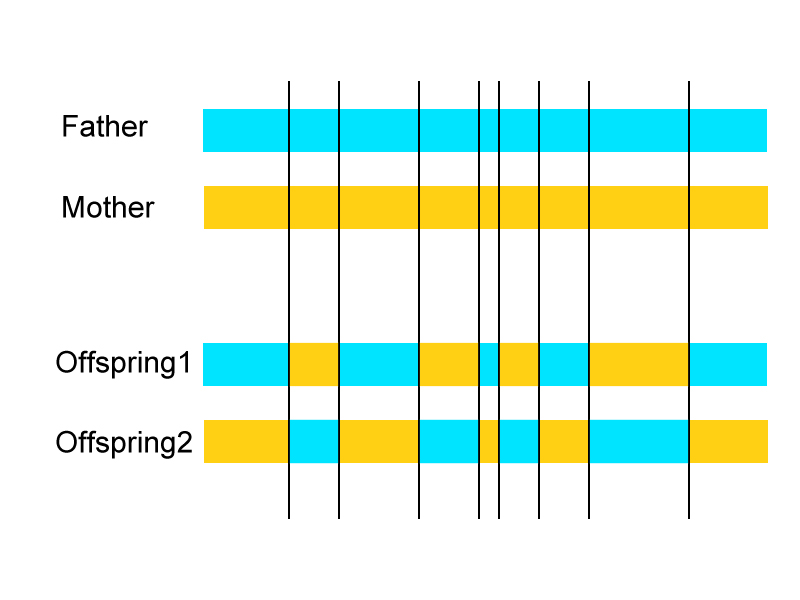
\includegraphics[width=1.0\columnwidth]{../images/crossover}\\[0.1cm]
    \caption{Crossover of parents}
    \label{figure:crossover}
\end{figure}

Figure \ref{figure:crossover} demonstrates the uniform crossover method introduced by \Citet{Spears1991, gwiazda2006crossover, ghosh2003advances}. This method uses a fixed ratio exchange rate between two parents to generate offspring. The black line indicate the exchange point in chromosome that are randomly selected by a random number generator.

For pattern adjustment, each individual is constituted by a group of different patterns, when two individual mates, crossover operation only performs on same pattern in both side of parents. For example, crossover operation can only be performed on two parent ``Front'' pattern to generate two offspring ``Front'' patterns. The crossover operation is summarized in Algorithm \ref{algorithm:crossover}.

\begin{algorithm}
\caption{Crossover}\label{algorithm:crossover}
\begin{algorithmic}[1]
\Procedure{Crossover}{Two individuals $ind_{1}$, $ind_{2}$, crossover rate $cxpb$}
	\If{$cxpb > random()$}
	\For{same block($b_1$,$b_2$) in $ind_{1}$ and $ind_{2}$}
		\State $N \gets$ number of control point in current block
		\For{$i=0;i< N;i++$}		
			\If{$rand()<0.5$} 		
				\State $offspring_{1_{i}} \gets b_{1_{i}}$
				\State $offspring_{2_{i}} \gets b_{2_{i}}$
			\Else
				\State $offspring_{1_{i}} \gets b_{2_{i}}$
				\State $offspring_{2_{i}} \gets b_{1_{i}}$
			\EndIf		
		\EndFor
	\EndFor
	\EndIf
\EndProcedure
\end{algorithmic}
\end{algorithm}

Because crossover only operates on the existing gene pool that is comprised by genes from two parents. It samples the area near their parents much more denser than mutation does. A higher crossover rate will increase the speed of convergence. In real world, a species will extinct without introducing new gene because the limited gene pool will be exhausted during the new born of the individuals. In genetic algorithm, this phenomenon appears as the over dense sampling into a local area around the initial population. This often results premature termination of the evolution. 

Mutation is a process that new genes can be introduced into the gene pool so that the diversity of the gene pool is enriched and gene degradation can be avoided. In genetic algorithm, mutation can explore new area of the cost surface much more efficient than crossover. \Citet{haupt2004practical} indicates that two issues should be taken into the consideration when performing mutation operation to an individual, the type of the mutation and the rate of the mutation. \Citet{Grefenstette4075583, Srinivas286385} point out that the choice of the mutation rate is heavily problem specified. For different problems, best mutation rate varies significantly, it needs to be set empirically for each particular problem. 

When performing genetic algorithm, a high mutation rate enlarges the searching range on the cost surface, whilst prevents the population to converge to a specific point. In the meantime, a very low rate of mutation will leads to a premature convergence very easily. According to the work of  \Citet{Yaman5653114}, in different stages of the the evolution, the genetic algorithm usually requires different exploration-exploitation ability. In this thesis, the non-uniform mutation, which presented by \Citet{michalewicz1996genetic}, is applied, in which the possible impact of mutation to an individual decreased when generation evolves. 

When initializing the initial population from seeds, a very wide distribution over the sampling cost surface is preferred, therefore, large mutation rate is set. Before evolution comes to the end, exploitations is much preferred than exploration so that the convergence can be ensured. At this stage, a high mutation rate will disturb the convergence of the algorithm. In the implementation of this algorithm, the mutation rate starts from 0.6 and decreased linearly by 0.002 for every generation that has evolved. Assume that $Gen_{max}$ is the predefined maximum number of generations of evolution. Then, for each individual, the randomly chosen chromosome $cp_{i}$ is replaces by one of the two values demonstrated in Equation \ref{equation:mutation},

\begin{equation}
cp_{i} = \left\{
\begin{matrix}
cp_{i} + \Delta(gen, t)   & if & \gamma \geq  0.5\\
\\
cp_{i} - \Delta(gen, t)   & if& \gamma  <  0.5\\
\end{matrix}\right.
\label{equation:mutation}
\end{equation}

where, $gen$ denotes the index of the current generation,  $\gamma$ is a normally distributed random number from 0 to 1, $\Delta(gen, t)$ is a random variable that mutates $cp_{i}$ in range $[0, t]$. The value of $\Delta(gen, t)$ is determined by the index of current generation $gen$ by Equation \ref{equation:mutation_factor}, introduced by \cite{michalewicz1996genetic},

\begin{equation}
\Delta(gen, t) = t * \left ( 1 - \lambda^{\left (1 - \frac{gen}{Gen_{max}}\right )^{r}} \right ) 
\label{equation:mutation_factor}
\end{equation}

where, $\lambda$ is an normally distributed random value from 0 to 1, $Gen_{max}$ is the maximum number of generations of the evolution. The exponential factor $r$ controls the influence of $gen$ on the distribution of $\Delta(gen, t)$ within its range. In which this operation becomes an uniform mutation if $r = 0$. The mutation process is introduced in more detail by Algorithm \ref{algorithm:mutation}

\begin{algorithm}
\caption{Mutation}\label{algorithm:mutation}
\begin{algorithmic}[1]
\Procedure{Mutation}{Individuals $ind$, Generation index $gen$, Mutation rate $mutpb$}
	\If{$mutpb > random()$}
	\For{$block_{i} \in ind$}	
		\State $dpb \gets random()$
		\State $U \gets$ the number of control point on $U$ direction		
		\State $V \gets$ the number of control point on $V$ direction	
		\If{$dpb<0.5$} \Comment{Variate $cp_{i}$ in $U$ direction}			
			\For{ Each row of $cp_{j}$ on $block_{i}$} 		
				\State Append $u$ value of $cp_{j}$ into array $Variables$
			\EndFor
			\LongState{Apply Equation \ref{equation:mutation} to each element in $Variables$ and evaluate the newly formed $Variables'$}
			\If{$Variables'$ is invalid}	
				\LongState{Reapply Equation \ref{equation:mutation} to each element in $Variables$ and evaluate the newly formed $Variables'$ till $Variables'$ is valid}
			\EndIf
			\For{ Each row of $cp_{j}$ on $block_{i}$} 		
				\LongState{ Assign back $u$ value of $cp_{j}$ from corresponding element in $Variables$}
			\EndFor				
				
		\Else	\Comment{Variate $cp_{j}$ in $V$ direction}
			\For{ Each column of $cp_{j}$ on $block_{i}$} 		
				\State Append $v$ value of $cp_{j}$ into array $Variables$
			\EndFor
			\LongState{Apply Equation \ref{equation:mutation} to each element in $Variables$ and evaluate the newly formed $Variables'$}
			\If{$Variables'$ is invalid}	
				\LongState{Reapply Equation \ref{equation:mutation} to each element in $Variables$ and evaluate the newly formed $Variables'$ till $Variables'$ is valid}
			\EndIf
			\For{ Each column of $cp$ on $block_{i}$} 		
				\LongState{ Assign $v$ value of $cp_{j}$ with corresponding element in $Variables$}
			\EndFor	
		\EndIf		
	\EndFor
	\EndIf
\EndProcedure
\end{algorithmic}
\end{algorithm}

For each mutation, only one orthogonal direction is modified in either row wise or column wise. For example, this mutation operator performs on $U$ direction only for a selected row of the control points or on $V$ direction only for a selected column of the control points. The choice between two directions are randomly selected for each block. For each row of the block, The mutated $U$ value of each control point is stored into an array denoted as $U_{row}$. The original $U$ value of every control point is also stored into an array denoted as $U_{row}'$. For each pattern, its block is created as a rectangle nurbs plane that the pattern is inscribed to. Therefore the $U$ value of  each row or column of a block is in the same incremental or decremental order. this is demonstrated in Figure \ref{figure:mutation_evaluation}.

\begin{figure}[H]
	\centering
	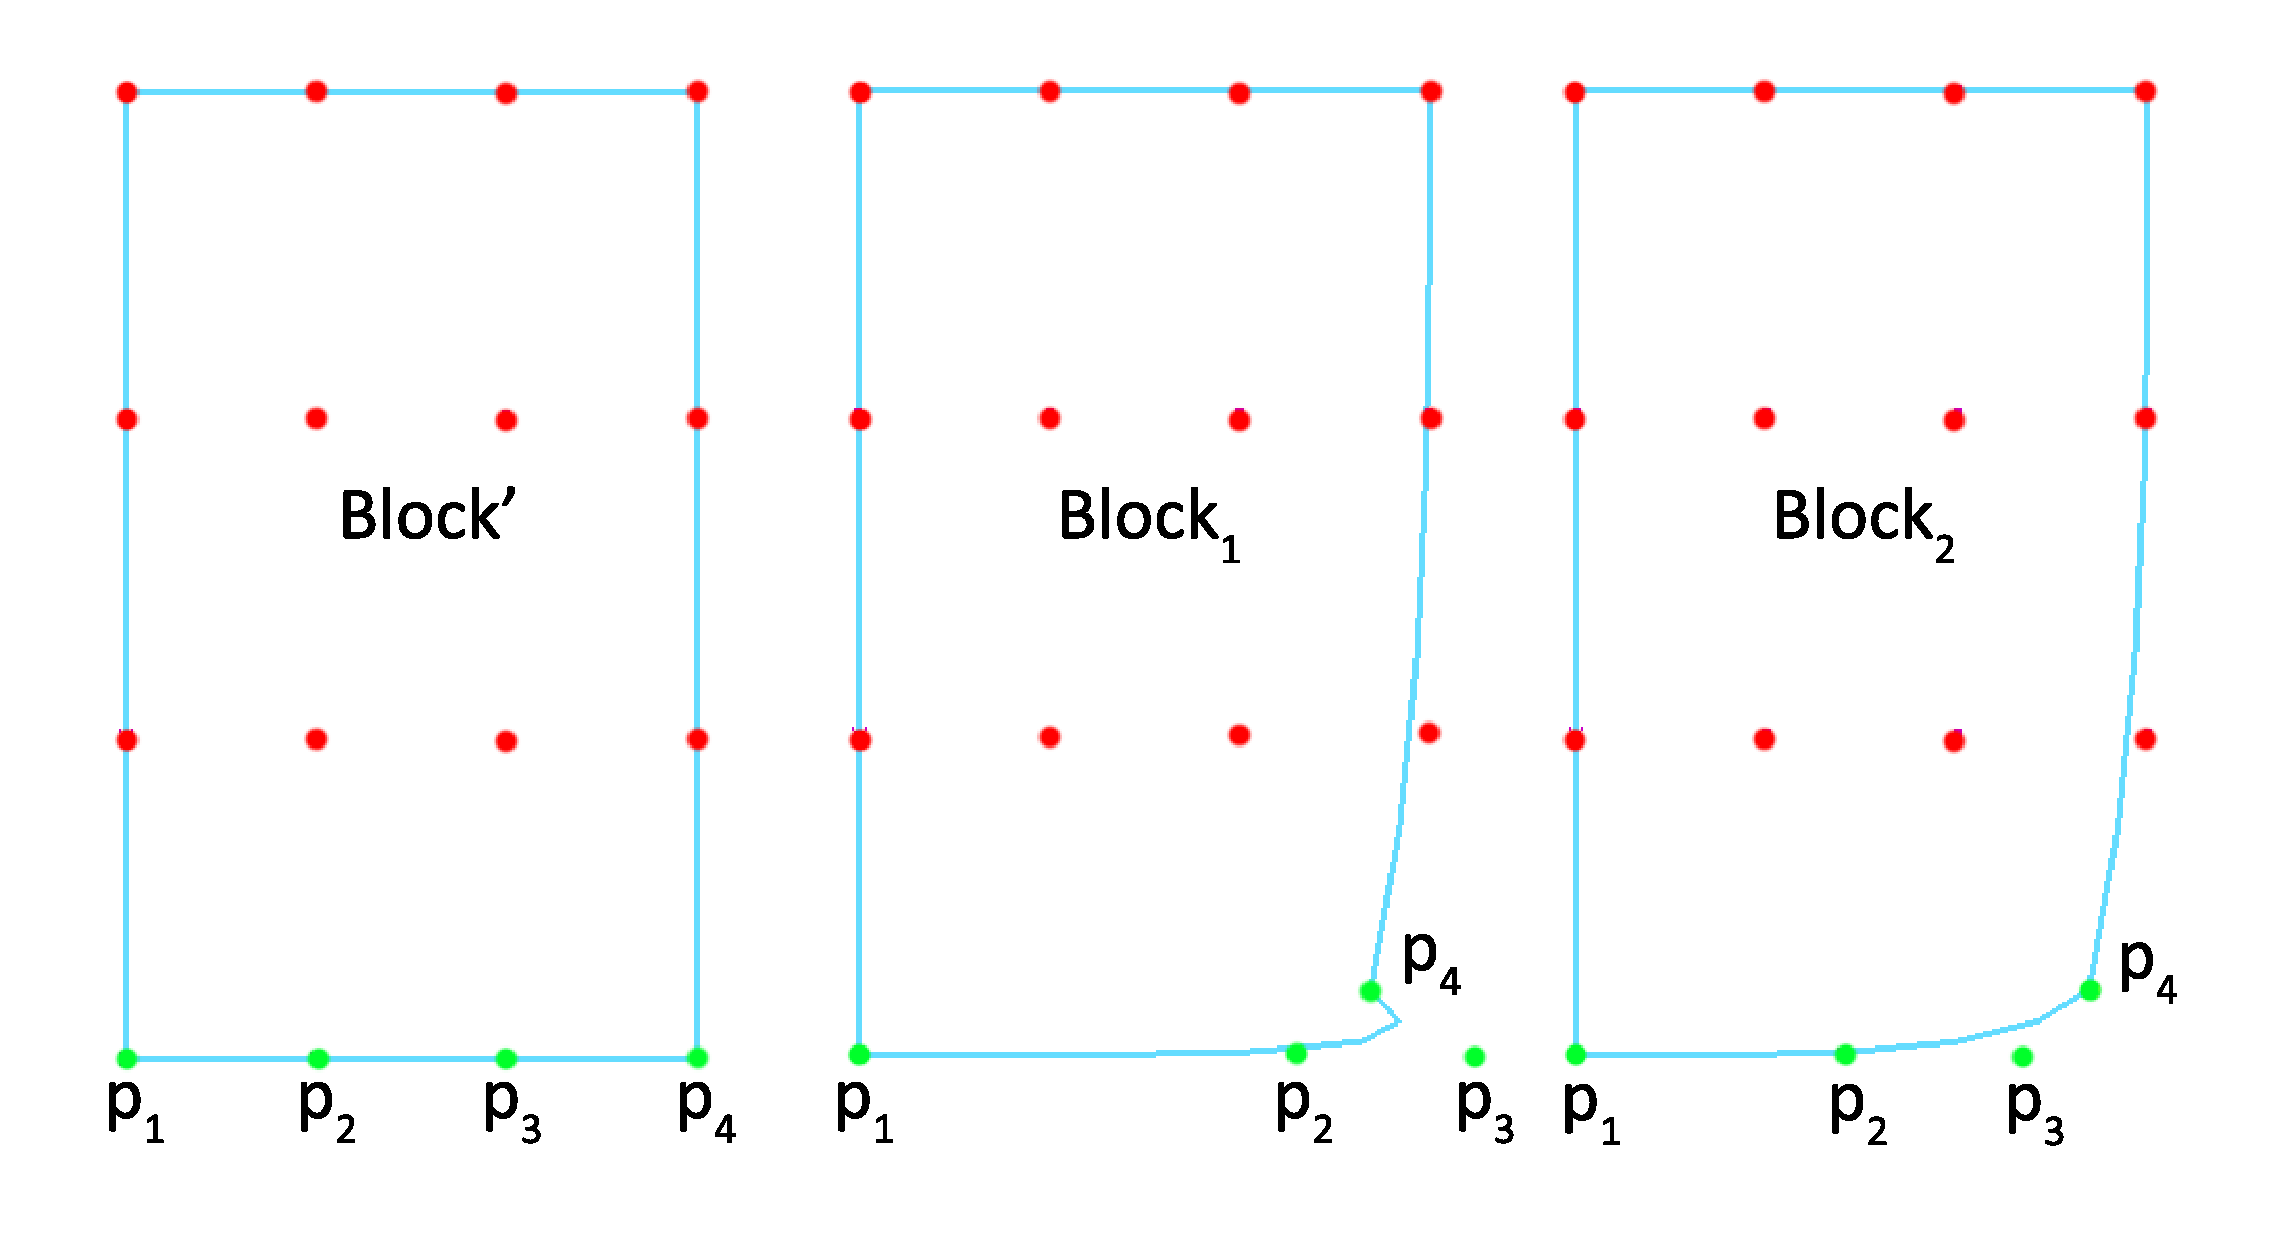
\includegraphics[width=1.0\columnwidth]{../images/mutation_evaluation}\\[0.1cm]
    \caption[Block mutation validation]{$Block'$ is at its initial status, $Block_{1}$ and $Block_{2}$ are the results from mutation operation applied on the bottom row of control points(green points).}
    \label{figure:mutation_evaluation}
\end{figure}

When a block is at its initial status, such as $Block'$ indicated in Figure \ref{figure:mutation_evaluation}, the order of the control points in the selected row is denoted by $R' = [p_{1}, p_{2}, p_{3}, p_{4}]$. $Block_{1}$ and $Block_{2}$ are two possible results generated by mutation operation on $Block'$. Sorted by the $U$ coordinate, the order of the control points in the corresponding row can be written as $R_{1} = [p_{1}, p_{2}, p_{4}, p_{3}]$ and $R_{2} = [p_{1}, p_{2}, p_{3}, p_{4}]$. In order to avoid face overlapping on a cloth pattern during mutation, the order of control points in any row or column need to be maintained. Since $R' \neq R_{1}$ and $R' = R_{2}$, $Block_{1}$ is marked as an invalid gene for current individual. In order to model cloth, each pattern need to be triangulated first to from the polygon from the outline of the pattern. In the case of $Block_{1}$, because the order in $R_{1}$ is changed, it will cause faces overlap to each other during the triangulation of the pattern.  When a pattern is invalided, mutation needs to be reapplied till $R' = R_{1}$. In this case, $Block_{2}$ is a valid gene of the current individual. 

\subsection{Evaluation and Selection}

In genetic algorithm, fitness function(cost function) describes the objective of the problem.  Given a solution, the fitness function is used to measure how far the current solution is to the desired goal of convergence. When a population evolves into a new generation, the selection operator deletes the $n$ worst individuals and breeds $n$ new individuals from the best individuals. In order to perform such a process, each individual need to be awarded a rank to indicate how close it comes to the ideal solution, ranking is generated by applying fitness function to each solution. In this algorithm, objectives for evolution is to adjust size and shape of the each pattern so that each pattern fulfil the requirement of the measurement criteria . Also, among patterns, the topology of the seam-line where two patterns are joint together remains. Most importantly the consistency of cloth design must be retained after resizing. Therefore, three fitness functions are developed for evaluating the fitness for each individual respectively.

\subsubsection{Measurements evaluation}
Given a block, landmarks are associated with datum points on the body of character. To create a block which follows the correct measurements, the distance between two landmarks of the block and their associated measurements should be equal. Therefore, the fitness function for the measurement objective can be described as Equation \ref{equation:measurement_f}.

\begin{equation}
Error_{m} = \frac{\sum_{i} \left \| M_{n} - Dist(l_{i_{s}}, l_{i_{e}}) \right \|}{n}
\label{equation:measurement_f}
\end{equation}

Where $M_{i}$ denotes the $i$th measurements associated with current block.  $l_{i_{s}}$ and $l_{i_{e}}$ are two landmarks on the block that are associated with $M_{i}$. $n$ denotes the number of the measurements that determines the size of the current block $b_{m}$. Because cloth pattern is a 2D surface, euclidean distance between two landmarks is used to compare with the measurement resulted by measurement method presented in previous chapter.

\subsubsection{Seam-lines evaluation}

A cloth cannot be made into the right design without correct sewing. It is the most important method that joints two piece of textile together. \Citet{reader2010new} defines a stitch as a single loop of thread that on the textile and sewing is the craft of fastening objects using stitches. 

In this thesis, a stitch refers to a constrain that attaches vertices on two patterns together and a seam-line is comprised by a group of stitches that from one end of the seam-line to another. Unless the design requires, normally, for a pair of seam-lines, the structure of both seam-lines are identical in order to form a flat and smooth pattern to pattern transition. Therefore, in this algorithm, two criteria is evaluated for seam-line evaluation, which are angle difference for each pair of point and length of corresponding edge on either side of a seam-line. 

\begin{figure}[H]
	\centering
	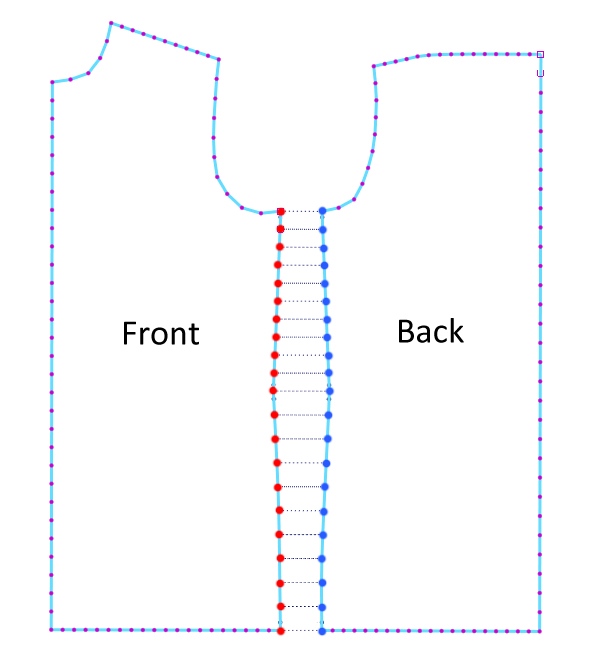
\includegraphics[width=0.7\columnwidth]{../images/seam_line}\\[0.1cm]
    \caption[A seam-line on patterns]{Seam-lines between ``Front'' pattern and ``Back'' pattern. The red points indicate the seam-line on the front pattern and blue points are the seam-line on the back patter.}
    \label{figure:seamline}
\end{figure}

Let $sline_{f}$ denotes a seam-line on ``Front'' pattern that depicted by the red points and $sline_{b}$ denotes a seam-line on ``Back'' pattern that depicted by the blue points in Figure \ref{figure:seamline}. For each pair of points that connected by a constrain have the same index in its corresponding seam-line. Given a point $pf_{i}$ on $sline_{f}$, the greatest included angle $\theta_{f}$ between $\overrightarrow{pf_{i-1}pf_{i}}$ and $\overrightarrow{pf_{i+1}pf_{i}}$ is recorded. Next, the point at the same location on $sline_{b}$ is also recorded as $\theta_{b}$. The total angle difference of a seam-lines on a pattern comparing to the standard input pattern is used to evaluate the angle criteria and it can be calculated by Equation \ref{equation:measurement_angle}.

\begin{equation}
Error_{angle} = \sum_{i=0}^{n}(\left \| \theta_{i_{f}} - \theta_{i_{b}} \right \|)
\label{equation:measurement_angle}
\end{equation}

Where $n$ denotes the number of point pairs in a seam-line. The other criteria is the edge length in seam-line. For a pair of seam-lines with same arc length, different point distribution will results an undesired tension along the seam-line in which causes wrinkle to occur around the seam-line. Within every seam-line, all points are stored in an predefined order, thus in order to ensure the consistency of the distribution of points in a seam-line pairs, edge that connects two successive points in a seam-line needs to be identical to the one in the other seam-line. Therefore, the edge length criteria can be written as Equation \ref{equation:measurement_edge_length}.

\begin{equation}
Error_{edge} = \sum_{i=0}^{n-1}(\left \| l_{i_{f}} - l_{i_{b}} \right \|)
\label{equation:measurement_edge_length}
\end{equation}

Where $l_{i_{f}}$ denotes the length of edge $\overline{p_{i}p_{i+1}}$ in a seam-line and $l_{i_{b}}$ denotes the length of edge $\overline{p'_{i}p'_{i+1}}$ in another seam-line. $n$ denotes the number of points in a seam-line. Therefore, the seam-line evaluation outputs the cost as the sum of angle criteria and the edge length criteria as Equation \ref{equation:measurement_edge_length2}.

\begin{equation}
Error_{s} = \frac{Error_{angle} + Error_{edge}}{n}    
\label{equation:measurement_edge_length2}
\end{equation}

where $n$ denote the number of point in current seam-line.

\subsubsection{Shape evaluation}

\Citet{armstrong2000} points out a cloth design can be translated into a set of pattern with predefined shape and sewing sequence. The shape of each pattern is the critical factor that determines the shape of the cloth after patterns are assembled. The consistency of the shape for each pattern needs to be kept through out the evolution in order to ensure the cloth that fits to a character remains the same. The shape of a geometry can be described via many methods. In this thesis, the definition introduced by \Citet{Kendall1977} is used to define a pattern shape. \Citet{Kendall1977} defines shape as ``all the geometrical information that remains when location, scale and rotational effects are filtered out from an object''. In this algorithm, if the included angle on each corresponding crucial point is identical between two patterns, the shape of these two pattern is considered same. 

In this algorithm, during the evolution, the changes of all the inner angle on every point of the contour of a block is measured as the cost of shape evaluation. Figure \ref{figure:shape_evaluation1} demonstrates variations for each pattern, because when crossover and mutation is performed on a pattern, the location of each point on pattern contour is changed, which the shape of a pattern is changed consequently. 

\begin{figure}[H]
	\centering
	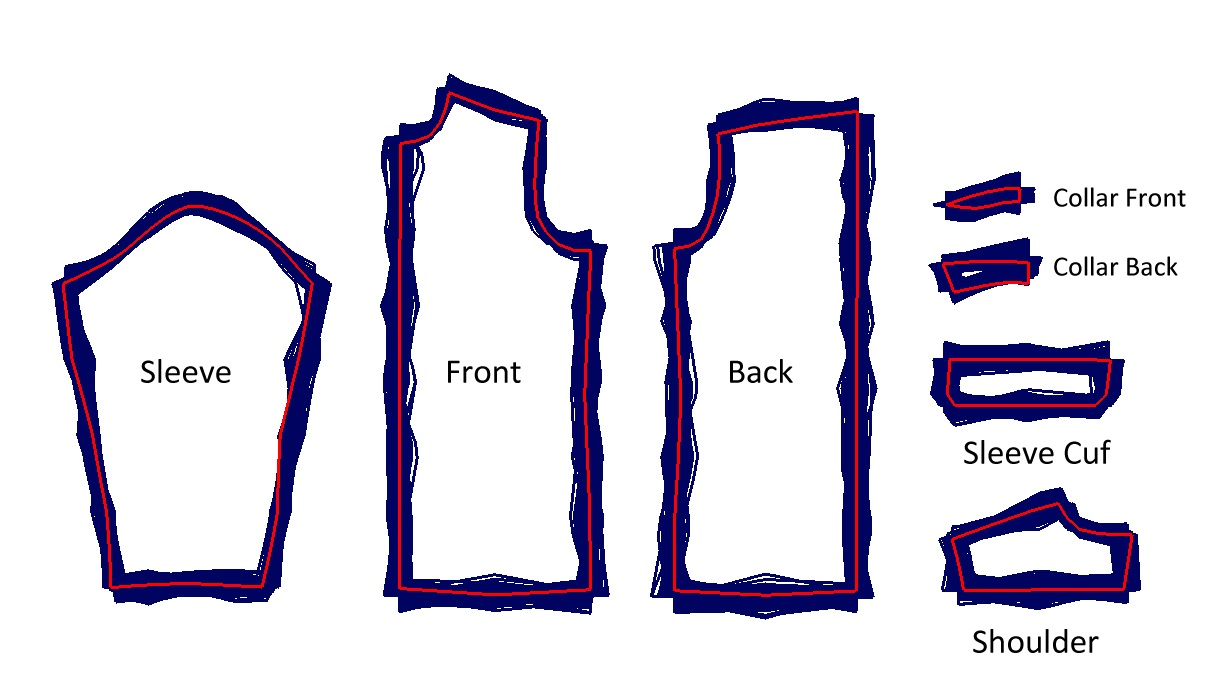
\includegraphics[width=1\columnwidth]{../images/MOP_shape_evaluation}\\[0.1cm]
    \caption[Shape evaluation for patterns]{Shape evaluation for the first generation patterns, Blue lines indicate the variations of the patterns, and the patterns that are indicated  by the red line has the best shape preservation.}
    \label{figure:shape_evaluation1}
\end{figure}


The pattern adjustment algorithm presented in this chapter solves a multi-objective optimization problem in which objectives conflict to each other. This optimization can only results a set of solutions called ``Pareto front'' instead of a single best solution. Within ``Pareto front'', each solution is not dominated (explained in following section) by the rest of the solutions within this set \Citep{michalewicz1996genetic}. However, lots of real problems in the real world are multi-objective problems that require a single solution. The common method for finding a single solution for a multi-objective optimization problem is that, multiple fitness function are used for the construction of ``Pareto front'', then a higher-level objective is used to find the ``best'' solution among ``Pareto front''. 

When adjusting a cloth, given a character, only one size of the cloth is needed for dressing the character. In order to select one solution from ``Pareto front'', only one or several non-conflict criteria can be used to select the ``best'' solution from ``Pareto front''. In this thesis, Preserving cloth style whilst fitting it to a different character is the main goal. therefore, the shape similarity between original pattern and resized pattern is used as the higher-level objective to select one solution from ``Pareto front''. When evolution limit is reached, all solutions in ``Pareto front'' are considered as ``good'' solutions to the character dressing problem. In other words, all patterns in ``Pareto front'' has achieved good fit and all seam-lines are consistent. Therefore, at this stage, the solution which has the least shape difference comparing to the original cloth patterns is selected as the final solution of dressing character. 

\begin{figure}[H]
	\centering
	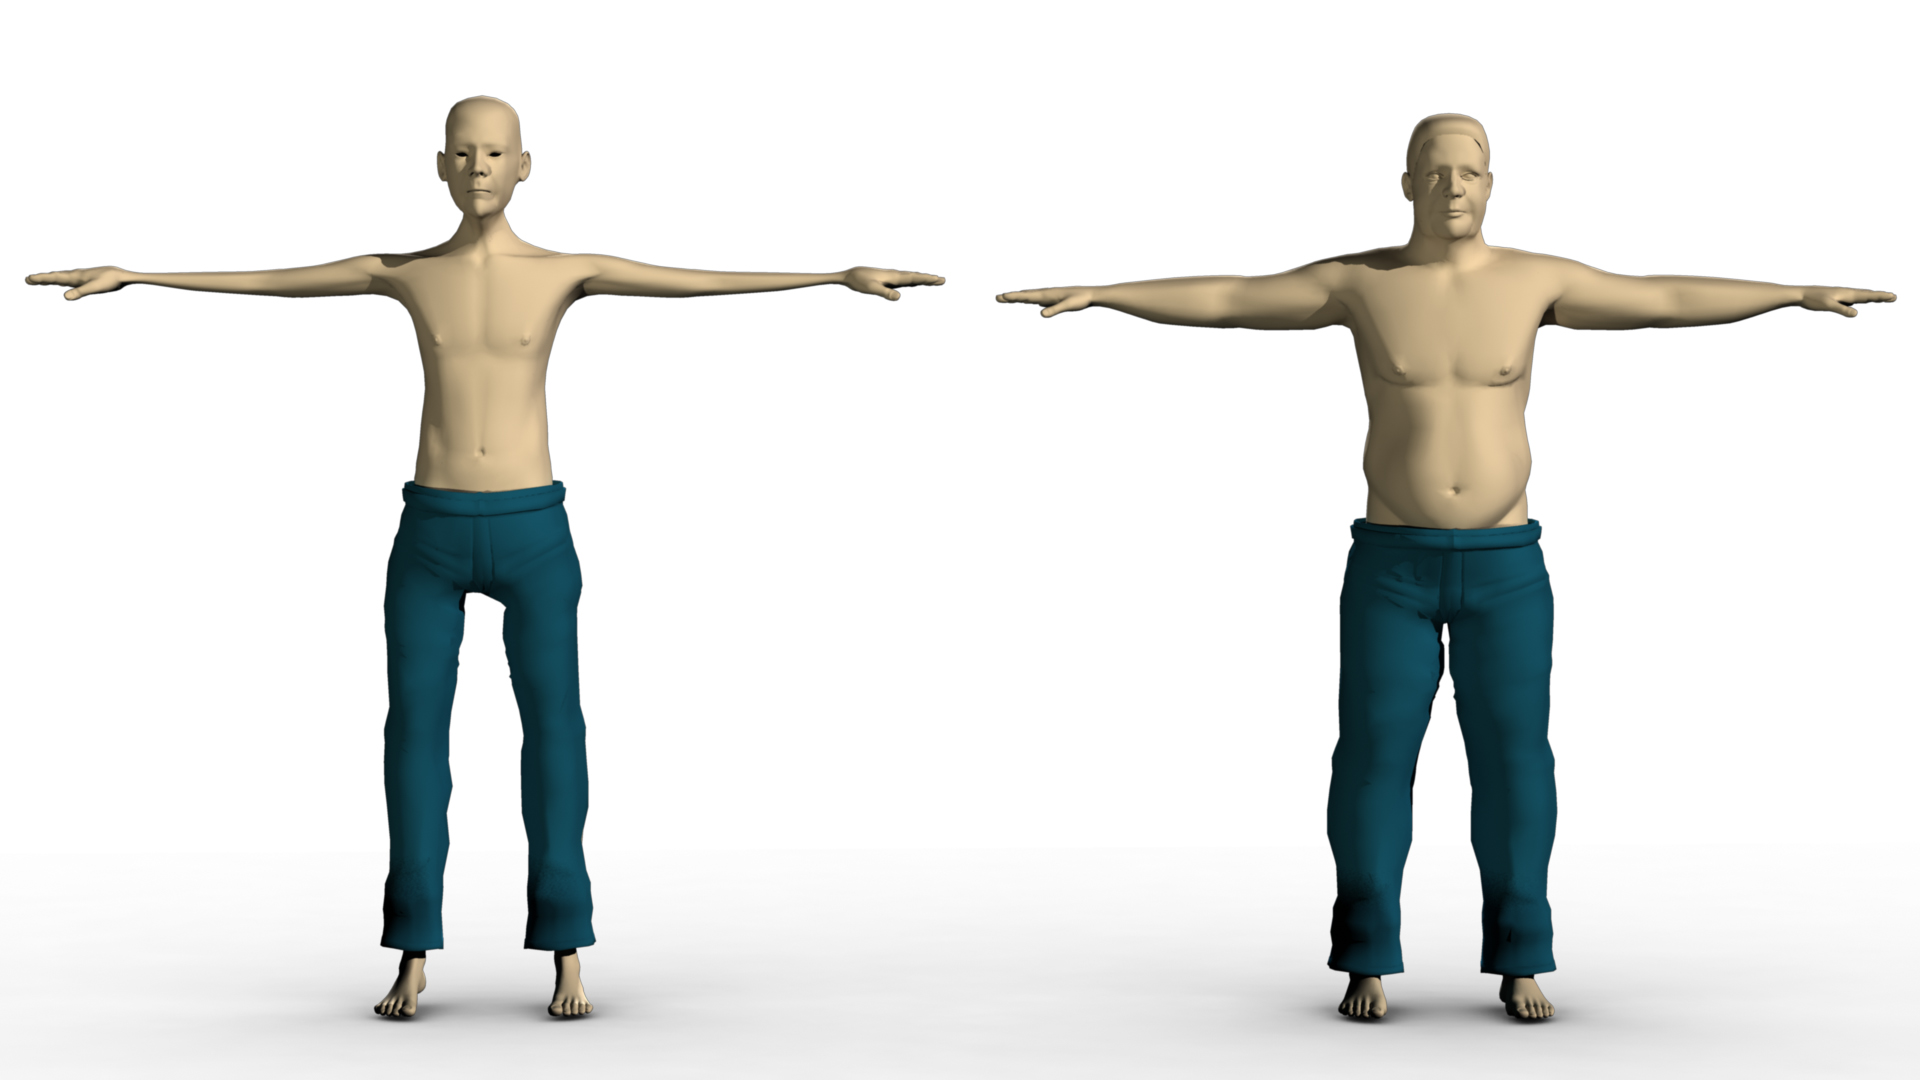
\includegraphics[width=1\columnwidth]{../images/sknny_fatty_fit_body}\\[0.1cm]
    \caption[Dressing two characters]{Character on the left has much thinner arms than character on the right.}
    \label{figure:character_compare}
\end{figure}

For the character on the left side, because the arm is much thinner than the one on the right, the arc length of the ``Arm hole'' is much shorter than the one on the right. However, two character have identical height, therefore, their shirt have the same back length. Figure \ref{figure:front_compare} demonstrates the ``Front'' pattern resized for the characters in Figure \ref{figure:character_compare}. The pattern is selected based on the minimum changes of inner angle of the ``critical point'' of the solutions. As demonstrated in Figure \ref{figure:fit_shirt_compare}, the design of the shirt is preserved. 

\begin{figure}[H]
	\centering
	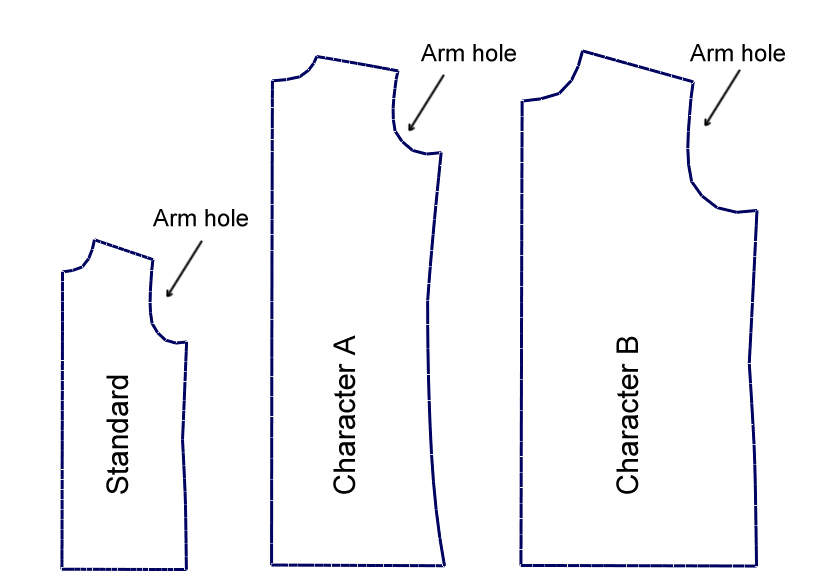
\includegraphics[width=1\columnwidth]{../images/sknny_fatty_front_pattern}\\[0.1cm]
    \caption[``Front'' pattern for both character in Figure \ref{figure:character_compare}]{The standard pattern(left), the ``Front'' pattern for the character on the left in Figure \ref{figure:character_compare}(middle), the ``Front'' pattern for the character on the right in Figure \ref{figure:character_compare}(right)}
    \label{figure:front_compare}
\end{figure}

\begin{figure}[H]
	\centering
	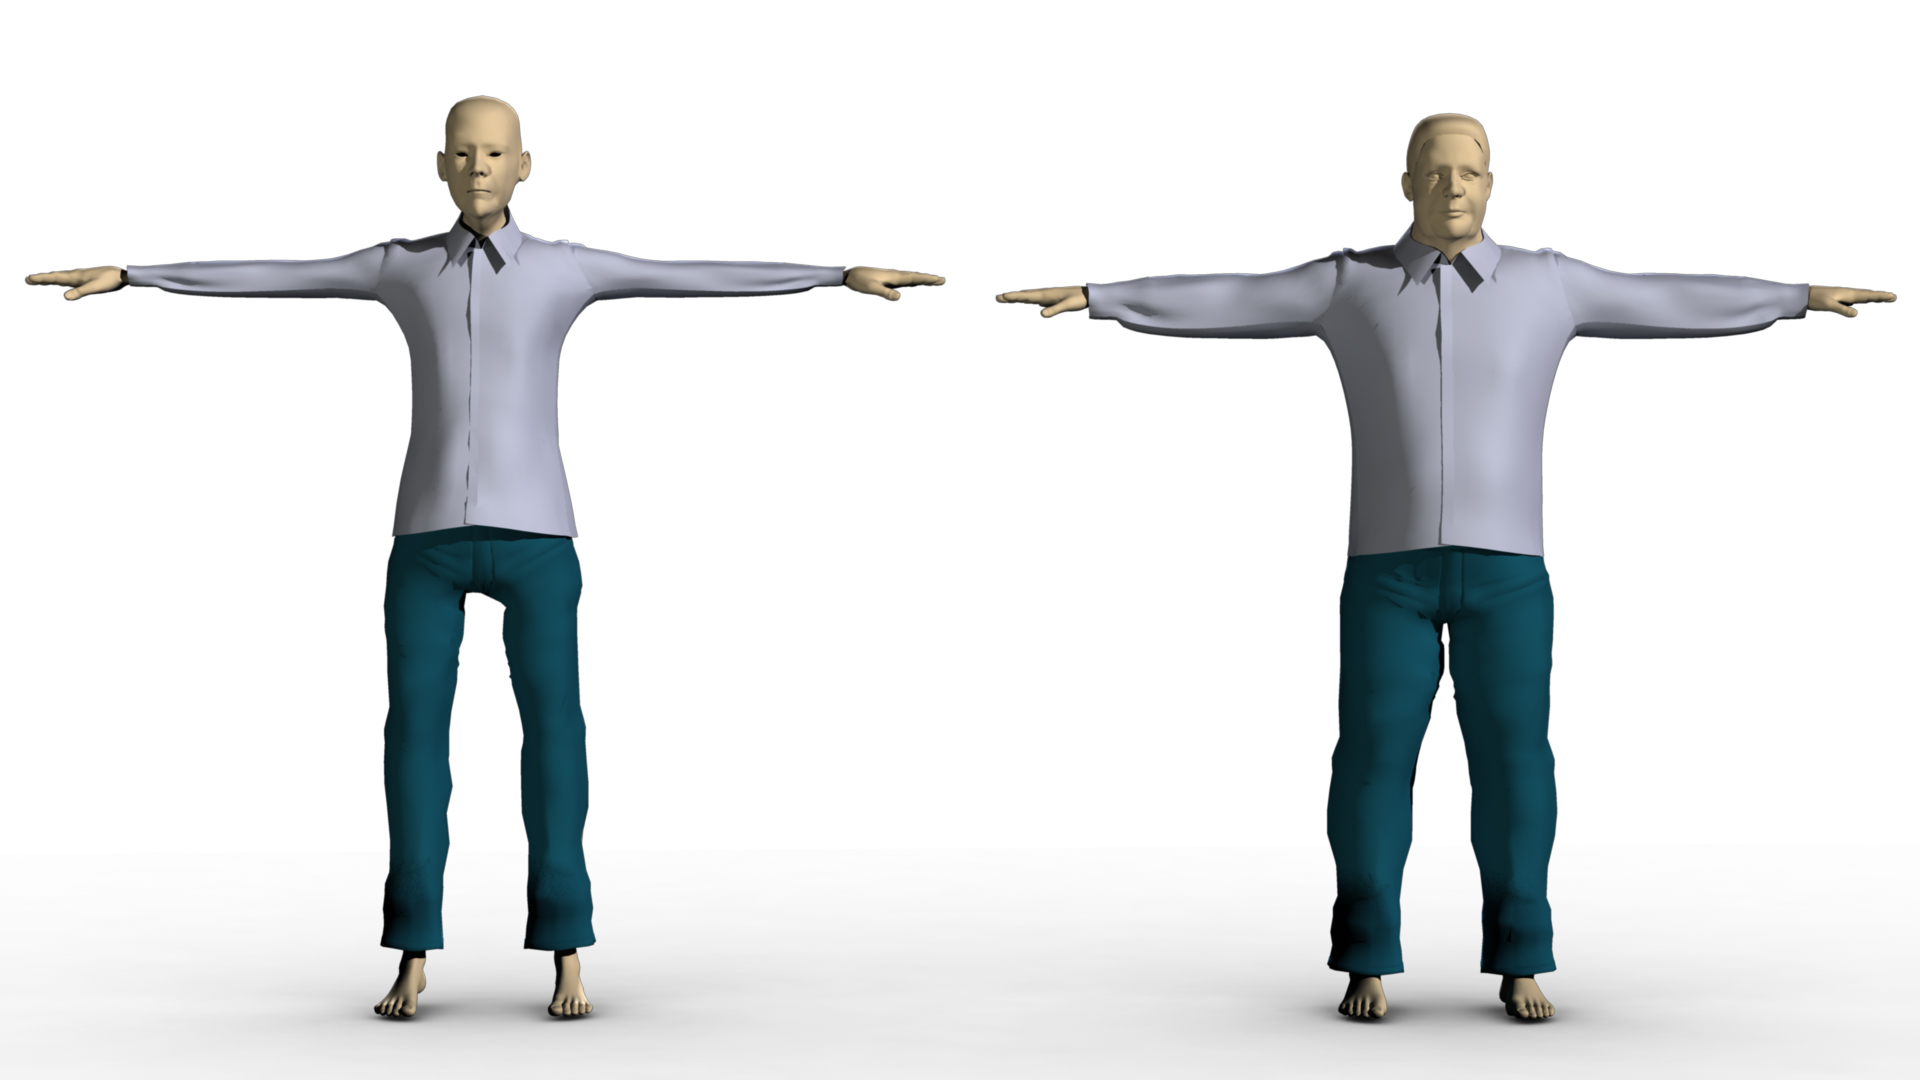
\includegraphics[width=1\columnwidth]{../images/sknny_fatty_fit_shirt}\\[0.1cm]
    \caption{Fit shirt modelled for characters}
    \label{figure:fit_shirt_compare}
\end{figure}

\subsubsection{Selection}

Selection decides individuals who are fit enough to survive the natural selection and reproduce child in next generation. In single objective optimization, solutions can be sorted according to the fitness to objective. However in multi-objective optimization, because objectives are usually conflict to each other, that is, when comparing two solution $A$ and $B$, $A$ may be better than $B$ in one objective but worse in another objectives at the same time. Therefore, the concept of domination is introduced into this area and two solution are compared by whether one is dominated by another. \Citet{deb2001multi} defines the concept of domination, that is, a solution $A$ is said to dominate solution $B$ , if following conditions are both true:

\begin{description}
  \item[Condition 1: ] The solution $A$ is not worse than solution $B$ in all objectives.  
  \item[Condition 2: ] The solution $A$ is strictly better then solution $B$ in at least one objective. 
\end{description}

To demonstrate the concept of domination, Figure \ref{figure::domination} illustrates an optimization problem with five solutions $s_{1}...s_{5}$ and two objectives $f_{1}$ and $f_{2}$.

\begin{figure}[H]
	\centering
	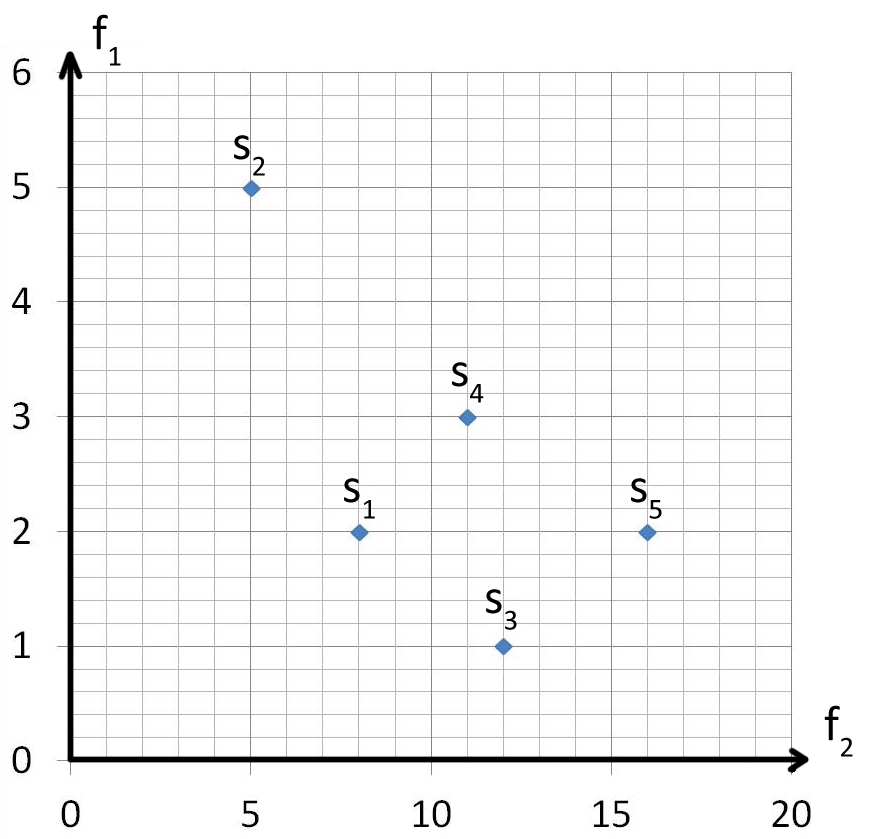
\includegraphics[width=0.9\columnwidth]{../images/domination}\\[0.1cm]
    \caption{Domination between five solutions}
    \label{figure::domination}
\end{figure}

$f_{1}$ and $f_{2}$ are two fitness functions for two objectives respectively where the $f_{1}$ needs to be minimized while $f_{2}$ needs to be maximized. In this case, two objectives $f_{1}$ and $f_{2}$ are equality important at all time, therefore it is impossible to select one best solution from this population according to both objectives. However, the definition of domination is able to decide the better solution among two solutions. As illustrated in Figure \ref{figure::domination}, when comparing $s_{1}$ and $s_{2}$, $s_{1}$ is better than $s_{2}$ in both $f_{1}$ and $f_{2}$. Thus, $s_{1}$ satisfy both conditions of the definition of domination and it can be said that $s_{1}$ dominates $s_{2}$. When comparing $s_{1}$ and $s_{5}$, $s_{5}$ is better than $s_{1}$ in $f_{2}$ but equals in $f_{1}$, this situation also satisfies both two conditions of the definition of domination, therefore, $s_{1}$ is dominated by $s_{5}$. When comparing $s_{4}$ to $s_{1}$, $s_{4}$ performs better on $f_{2}$ than $s_{1}$ but worse on $f_{1}$, therefore, $s_{1}$ and $s_{4}$ does not dominates each other. 

\Citet{Deb996017} introduced non-dominating sorting algorithm that utilises this method to select all solutions in a population that does not dominated by the rest of the population to construct ``Pareto front''. To be more specific, if there are two solutions that does not dominates each other, but each of them dominates the rest of the population, it can be said that, these two solutions are ``equally the best'' and the ``Pareto front'' is constituted by these two solutions.

In this case, after comparing all pairs of the solutions, it can be concluded that $s_{5}$ dominates $s_{1}, s_{2}, s_{4}$ as well as $s_{3}$ dominates $s_{1}, s_{2}, s_{4}$. Among $s_{3}$ and $s_{5}$, $s_{3}$ exceed $s_{5}$ in $f_{1}$ but dwarfed by $s_{5}$ in $f_{2}$. Therefore, $s_{3}$ and $s_{5}$ are non-dominated by each other but dominate the rest of the population. Consequently, ``Pareto front'' is constituted by $s_{3}$ and $s_{5}$. 

In this chapter, all solutions are compared according to the definition of domination in terms of three fitness functions, that is, measurements, seam-line and pattern shape to from ``Pareto front''. In the final step, the shape objective is used for selecting one solution with less shape distortion as the final solution for constructing cloth for characters. The general process for pattern resize genetic algorithm is summarized in Algorithm \ref{algorithm:pattern_resizing}.


\begin{algorithm}[H]
\caption{Pattern Resizing}\label{algorithm:pattern_resizing}
\begin{algorithmic}[1]
\Procedure{Evolve}{$pop$ denotes a population contains multiple pattern variations, $Npop$ denotes the number of individuals in $pop$ , $NGen$ denotes the max number of evolve generation}
	\For{gen in $NGen$}
		\State $parent$ = Selection( $pop$, len($pop$) )
		\State $offspring$ = Crossover( $parent$ )
		\State $mutated$ = Mutation( $pop$, $MutPb$ )($MutPb$ denotes mutation probability)
		
		\For{$individual$ in $offspring$}		
				\State $individual.fitness$ = Evaluation($individual$)
		\EndFor
		
		\For{$individual$ in $mutated$}		
				\State $individual.fitness$ = Evaluation($individual$)
		\EndFor
				
		\State $pop$ = $parent$ + $offspring$ + $mutated$
	\EndFor
\EndProcedure
\end{algorithmic}
\end{algorithm}

%To perform such a process, Assume $S_{pf}$ is the "Pareto front" produced by genetic algorithm for cloth resizing. Within each solution $s \in S_{pf}$, pattern $p_{i}$ is decoded from the block by  using the parametric coordinate of the block. In next step, standard principal components analysis(PCA) is used to extract geometrical feature of current pattern. Because all the pattern are represented by a two dimensional coordinate on the plane, therefore, two eigenvectors and two eigenvalues are result from PCA, the feature vector consists with two eigenvectors $FeatureVector = [eig_{l},eig_{s}]$ and two eigenvalue can be written as $\Lambda_{l}$ and $\Lambda_{s}$. The larger eigenvalue $\Lambda_{l}$ represents the variance of data along the major-axis of the shape. The difference between a pattern and its original pattern is calculated by Eq.\ref{}.
%
%\begin{equation}
%
%
%
%
%Error_{s} = \frac{Error_{angle} + Error_{edge}}{n}    
%\label{equation:measurement_seamline}
%\end{equation}




%**************************************************************************

\section{Pattern Assembling}

After every patten is adjusted into the correct shape and size based on the measurements from the character, they are ready to be placed on character and stitched together to form a complete cloth. In order to achieve such a task, all patterns are positioned onto 3D character simultaneously before sewing takes place. Three steps are involved for the construction of 3D cloth. Firstly, the bounding surface of each body part of character are created, then, patterns are triangulated and then based on the parametric coordinate of the bounding surface, all vertices on a 2D pattern are transferred onto bounding surface to form a 3D mesh. Finally, according to the seam-line information, constrains are created to every point pair in seam-lines and physical simulation is performed to to stitch patterns together to give the final shape of cloth.

Bounding surfaces are used as a guideline for transferring 2D cloth patterns into 3D mesh. Each pattern is responsible for covering certain part of character body, the bounding surfaces are used to position patterns on their corresponding body location. For human body, the general shape of each body section such as torso, legs or arms, is a cylindrical shape. For this reason, the cylindrical surface is chosen as the bounding surface. Moreover, cloth patterns are developable surface as they are cut out from a flat piece of textile materials. Therefore, construct a developable surface around the body of the character first and then transfer patterns that are also developable onto to it minimize the distortion during the pattern positioning process. 

In order to create bounding surface, character model is divided into six parts such as head, torso and four limbs. In this thesis, if the input character has skeleton attached to it, the body parts can be determined by the skin weight corresponding to each bone of the skeleton. If the character does not have skeleton, the body can be segmented interactively by user.

After body segmentation is completed, PCA is performed on each part of the body to calculate the principle vector of each body part. Then, by using the principle vector as the direction, central line of the each body is created as the central axis of the cylindrical bounding surface. The radius of  cylindrical bounding surface is then determined by the number of pattern associated with this body part. At this step, pattern are arranged on the flattened bounding surface side by side according to position of the sewing relationship as showed in Figure \ref{figure:pattern_and_boundingBox}. The width on the $U$ direction of all the patterns is the circumference of the bounding surface. Figure \ref{figure:sewing_bounding_surface} demonstrates all the bounding surfaces for a character.

\begin{figure}[H]
	\centering
	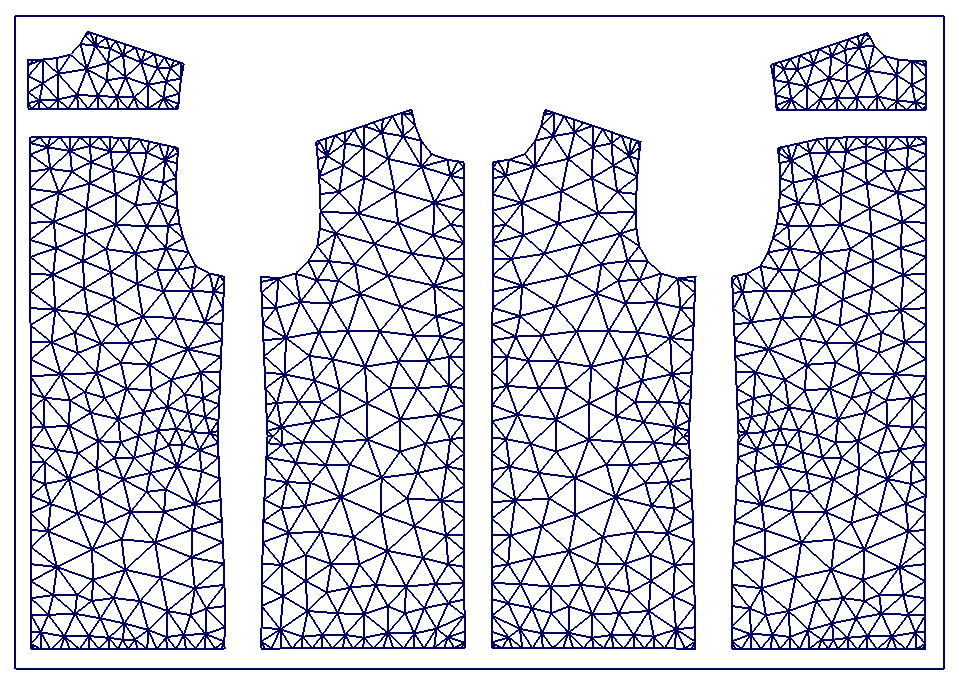
\includegraphics[width=0.95\columnwidth]{../images/pattern_and_boundingBox}\\[0.1cm]
    \caption[Patterns in a box]{Patterns arranged side by side within the range of a box, this box is the flattened bounding surface.}
    \label{figure:pattern_and_boundingBox}
\end{figure}

\begin{figure}[H]
	\centering
	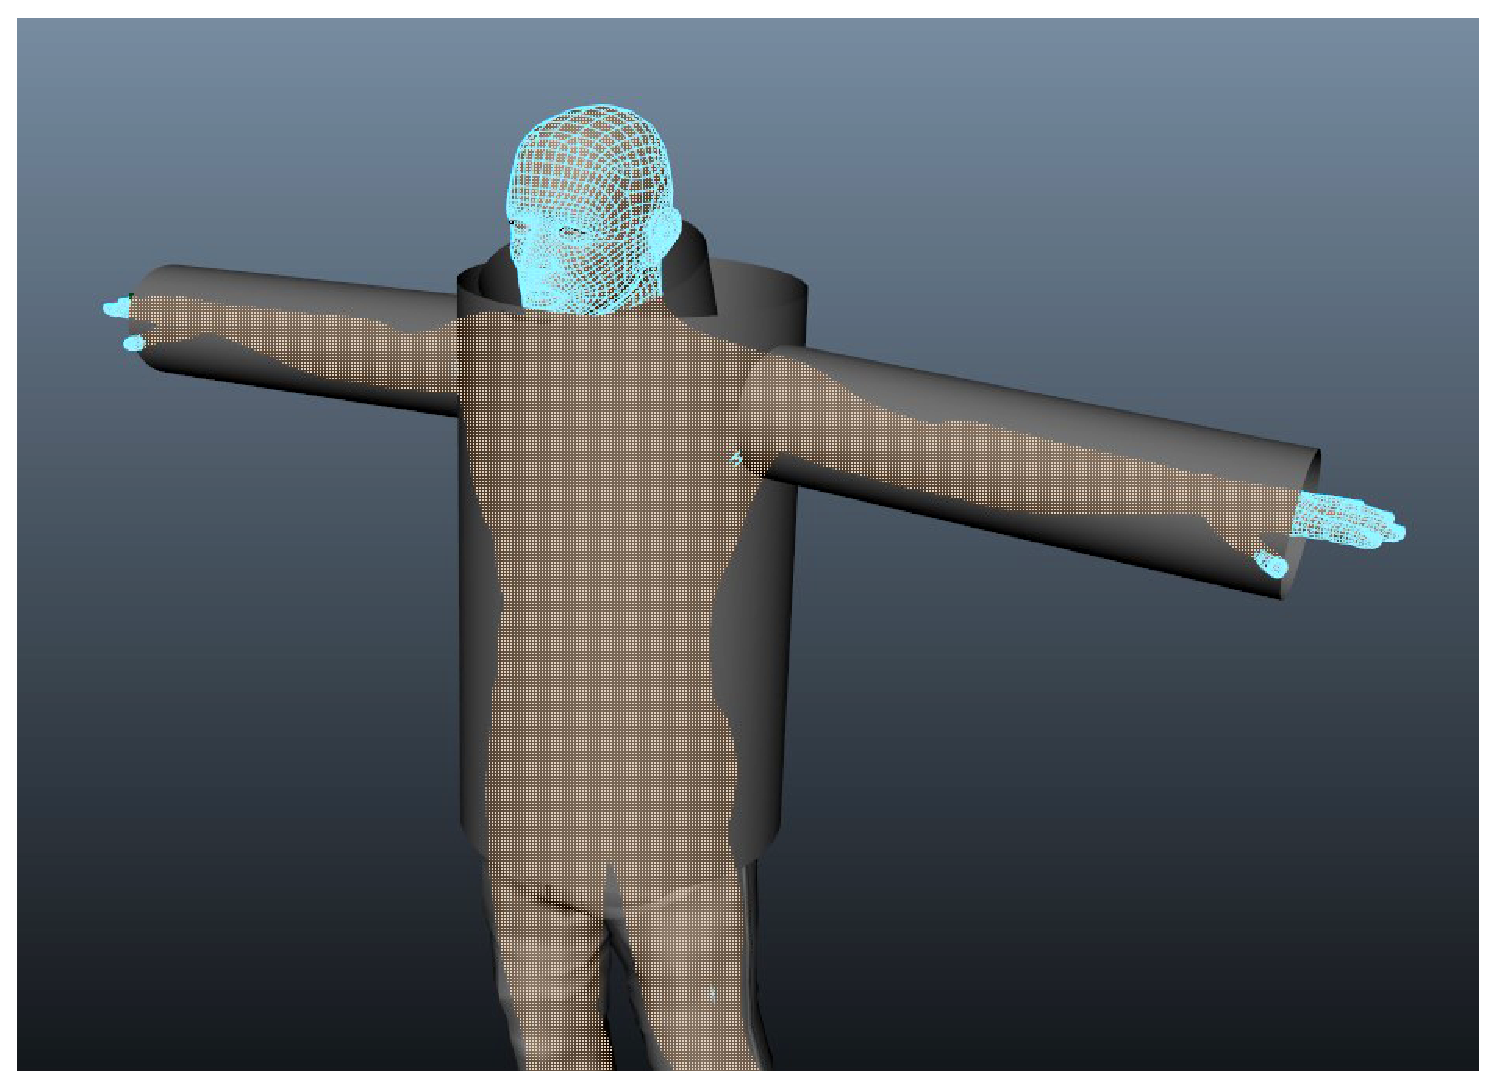
\includegraphics[width=0.9\columnwidth]{../images/bounding_surface}\\[0.1cm]
    \caption{ Bounding surfaces on character.}
    \label{figure:sewing_bounding_surface}
\end{figure}

In the next step, the vertices of the 2D pattern are transferred onto bounding surface. Based on the parametric coordinate of each point of 2D pattern on the flattened bounding surface, each point can be located by the same parametric coordinate on the cylindrical bounding surface. Finally, by applying the same topology structure to the points on bounding surface, 3D mesh be constructed from 2D cloth pattern. Figure \ref{figure:normal_patterns} demonstrate the fully positioned shirt patterns of a character.  

\begin{figure}[H]
	\centering
	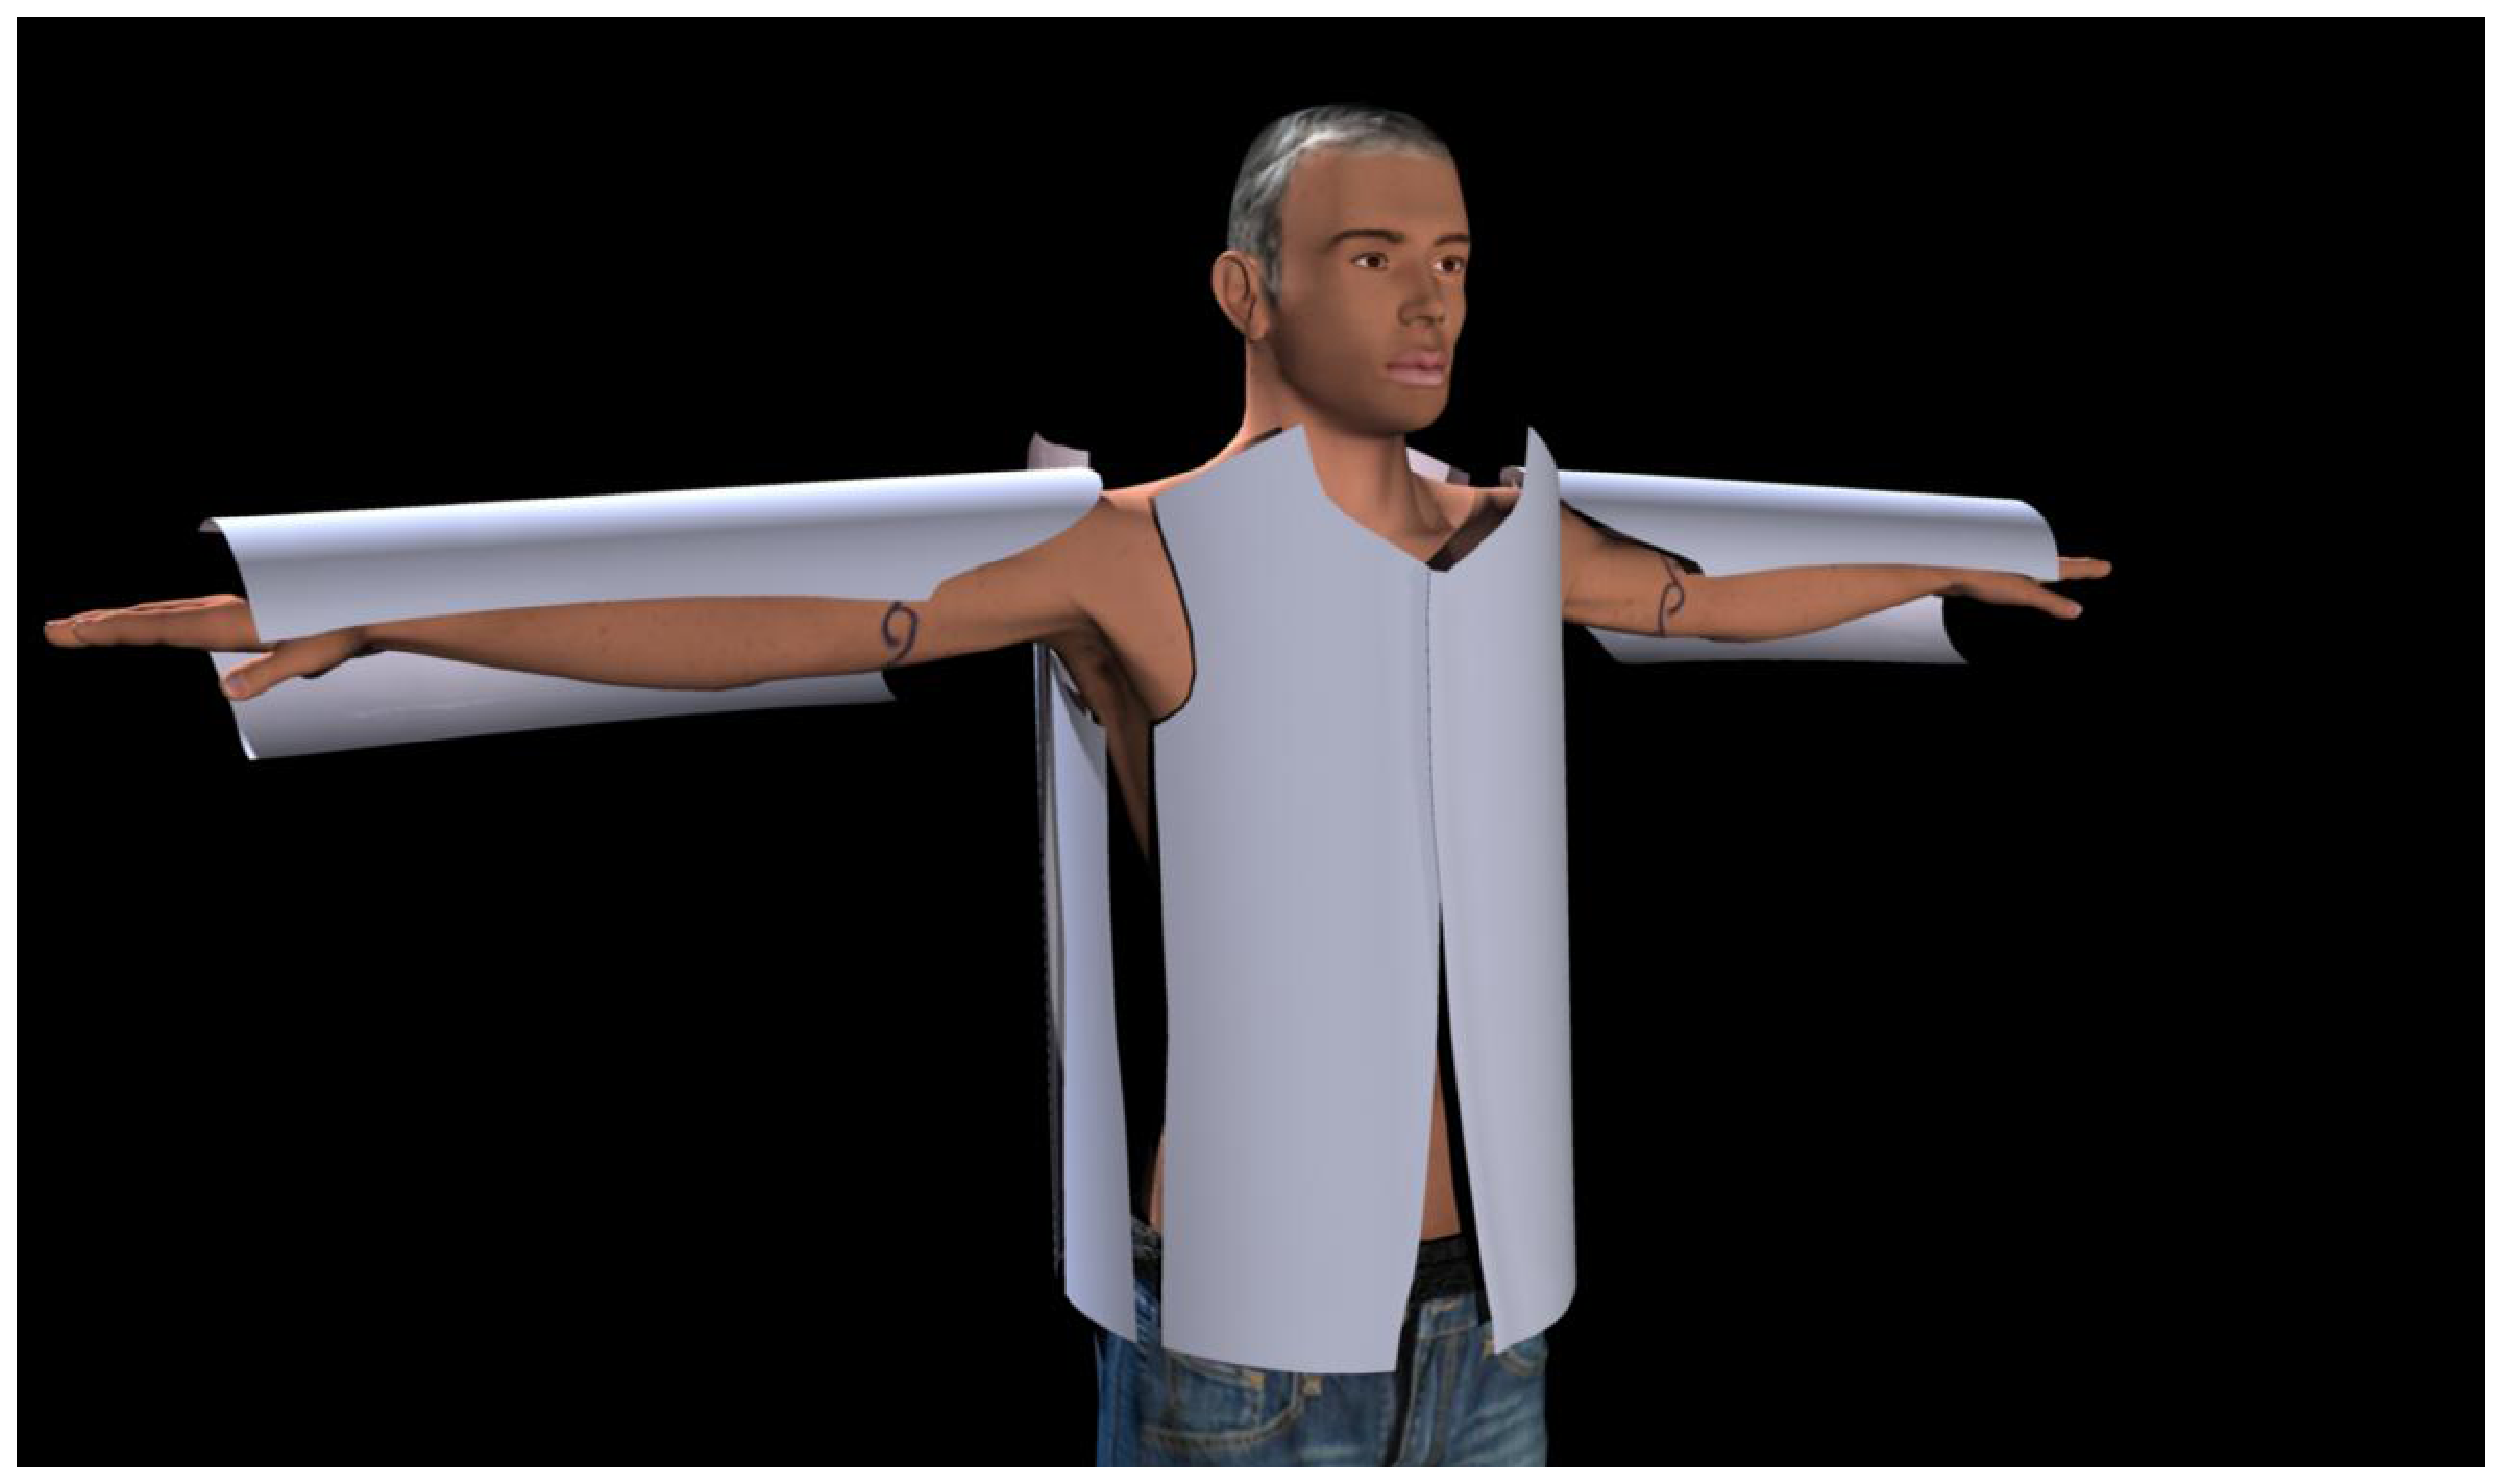
\includegraphics[width=1.0\columnwidth]{../images/normal_patterns}\\[0.1cm]
    \caption{3D patterns}
    \label{figure:normal_patterns}
\end{figure}

\begin{figure}[H]
	\centering
	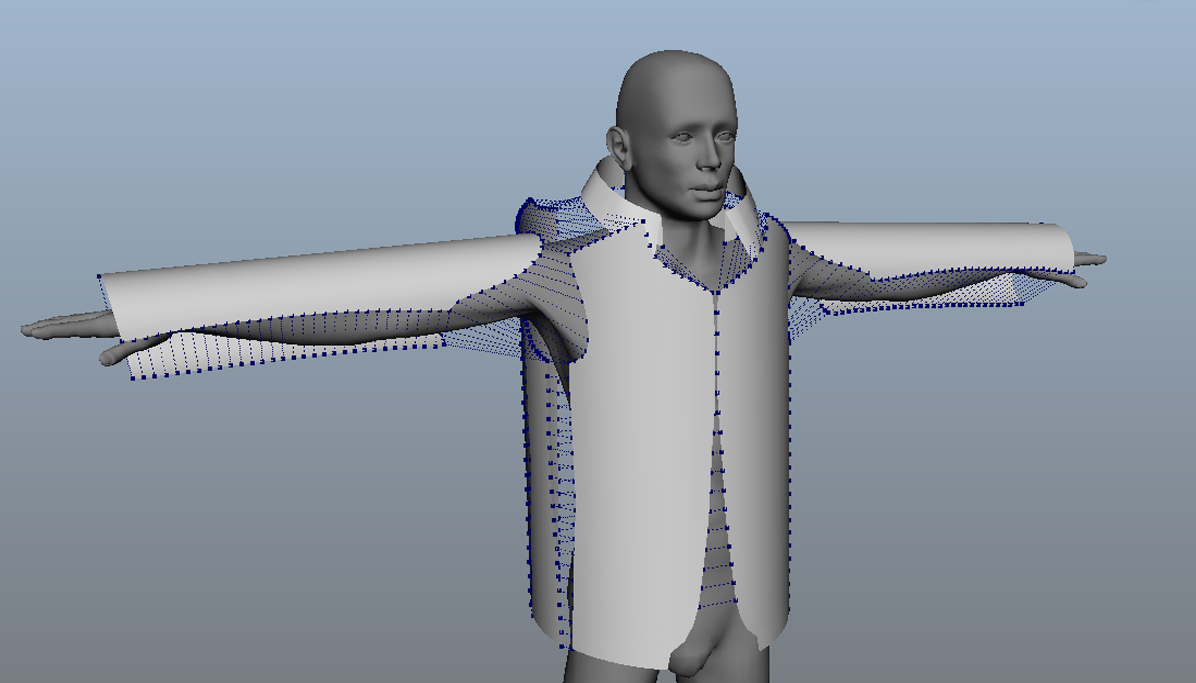
\includegraphics[width=1.0\columnwidth]{../images/sewing}\\[0.1cm]
    \caption{3D pattern sewing}
    \label{figure:sewing_constrains}
\end{figure}


In the final step, based on the seam-lines between each pattern, constrains are created between two points in a point pair on seam-line. Then physical simulation is performed to pull all the patterns together. In this thesis, the nCloth module in Maya2012 \Citep{maya2012} is used to perform the physical simulation. Figure \ref{figure:sewing_constrains} illustrates all the sewing constrains. 
 
In order to validate the algorithm presented in this chapter, a shirt design and a trousers design presented in \Citet{xiong2000} are used for dressing four different characters with largely different body shapes and proportions. This experiment is performed on an Intel Xeon 3.33GHz PC with 8GB RAM running Windows 7 (64-bit) operating system and Maya2012. For cloth pattern adjusting genetic algorithm, 400 initial solutions are generated at the beginning of the algorithm. For each character, 200 evolutions are performed. Figure \ref{figure:character_A_pattern}, \ref{figure:character_B_pattern}, \ref{figure:character_C_pattern} and \ref{figure:character_D_pattern} demonstrate the final results for each character respectively. Figure \ref{figure:final_result_front} and  \ref{figure:final_result_back} demonstrate the final cloth fit onto each character. Table \ref{table:GA_errors} lists out the fitness value of the final solution of all characters. Notices that for character A and D, because the body proportion is largely different from the standard human body proportion that the shirt pattern and trousers pattern are based on, cloth pattern requires larger deformation to fit the character A and D than character B and C. Therefore, the result of the shape evaluation for the patterns for character A and D is worse than the patterns for character B and C.

  
\begin{figure}[H]
	\centering
	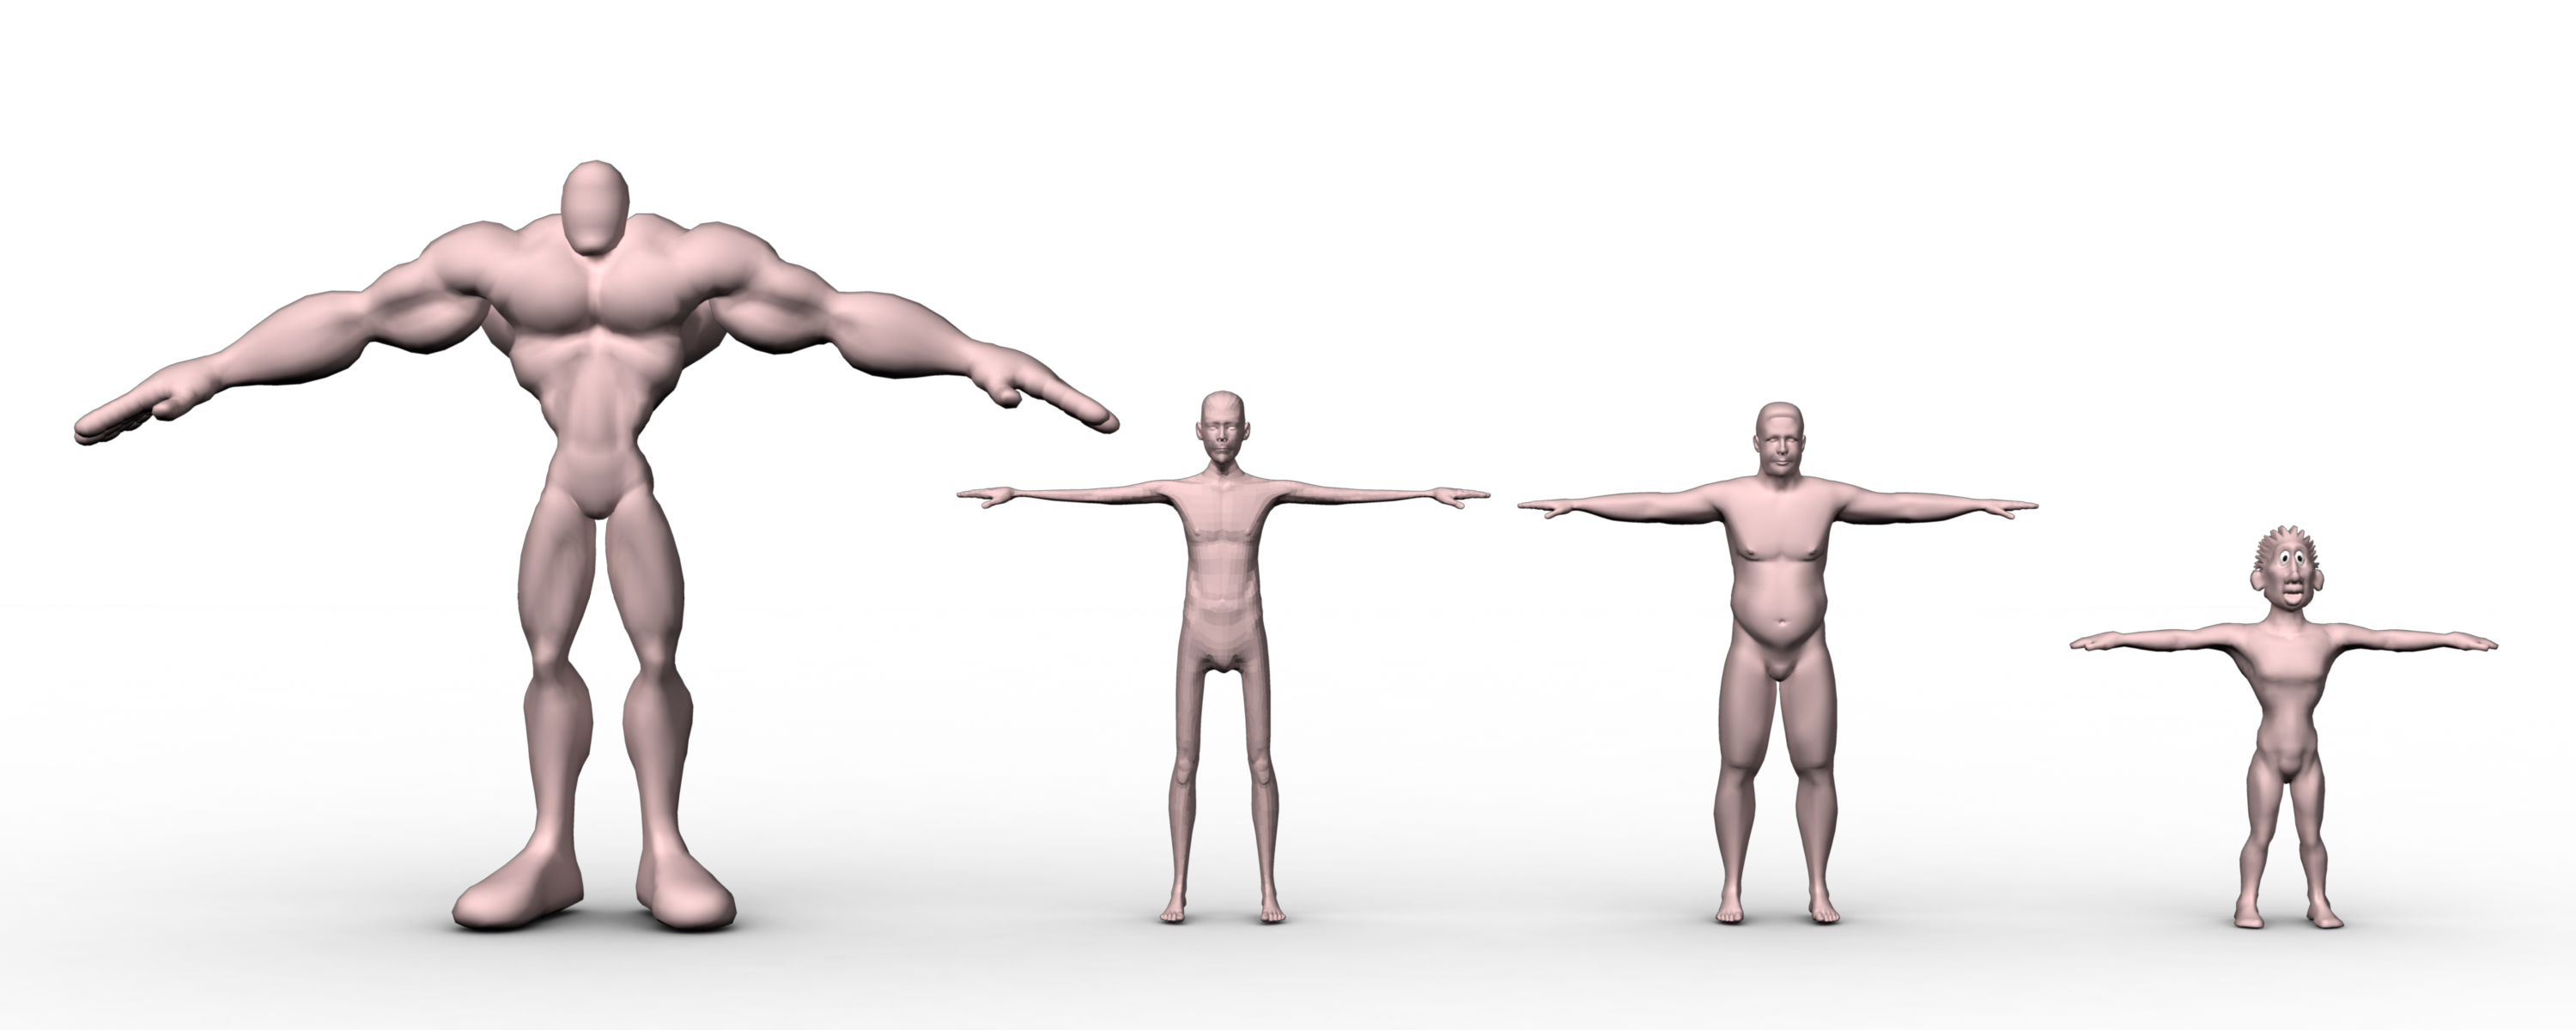
\includegraphics[width=1.0\columnwidth]{../images/all_characters}\\[0.1cm]
    \caption[Characters]{Four different characters used for the cloth modelling experiments, from left, Character A, B, C and D.}
    \label{figure:all_characters}
\end{figure}


\begin{figure}[H]
        \centering
        \begin{subfigure}[b]{0.7\textwidth}
                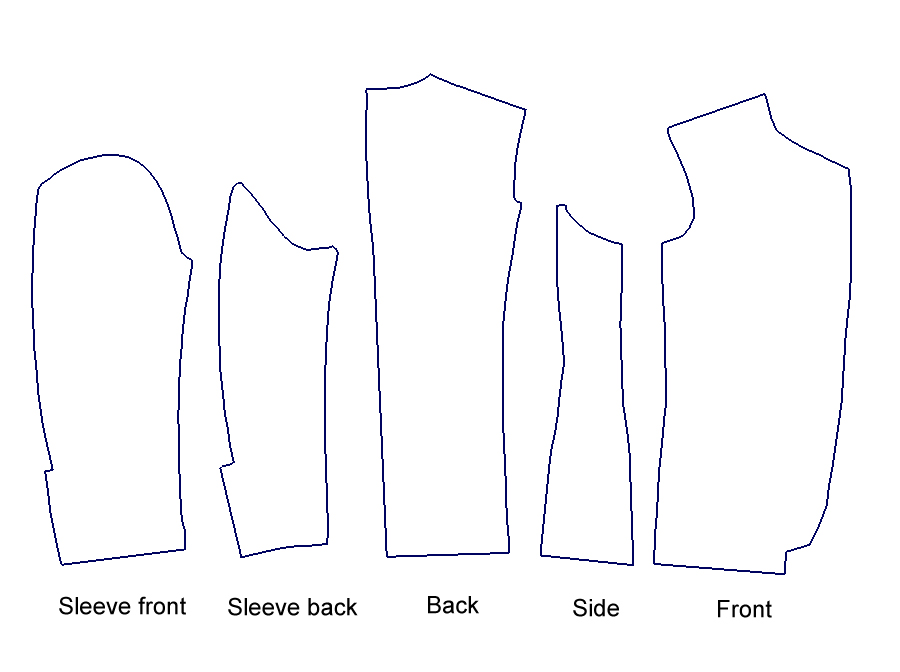
\includegraphics[width=\textwidth]{../images/shirt_pattern}
                \caption{}
                \label{fig:subjectA}
        \end{subfigure}%
        ~ %add desired spacing between images, e. g. ~, \quad, \qquad etc.
          %(or a blank line to force the subfigure onto a new line)
        \begin{subfigure}[b]{0.3\textwidth}
                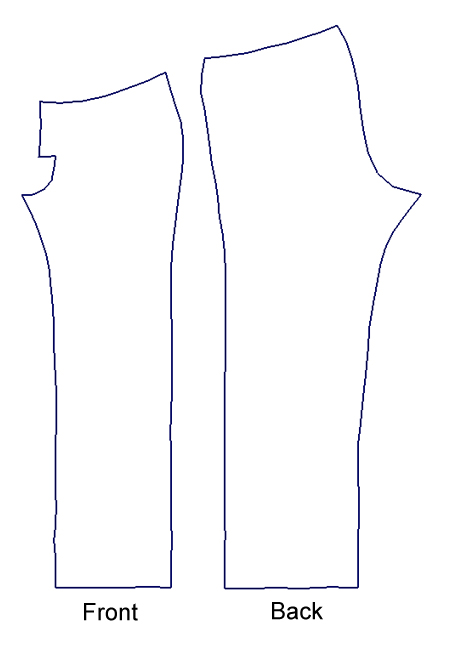
\includegraphics[width=\textwidth]{../images/trousers_pattern}
                \caption{}
                \label{fig:subjectB}
        \end{subfigure}
        \caption{Cloth patterns\Citep{xiong2000}, standard shirt patterns(left); standard trousers patterns(right)}\label{fig:patterns}
\end{figure}

\begin{figure}[H]
	\centering
	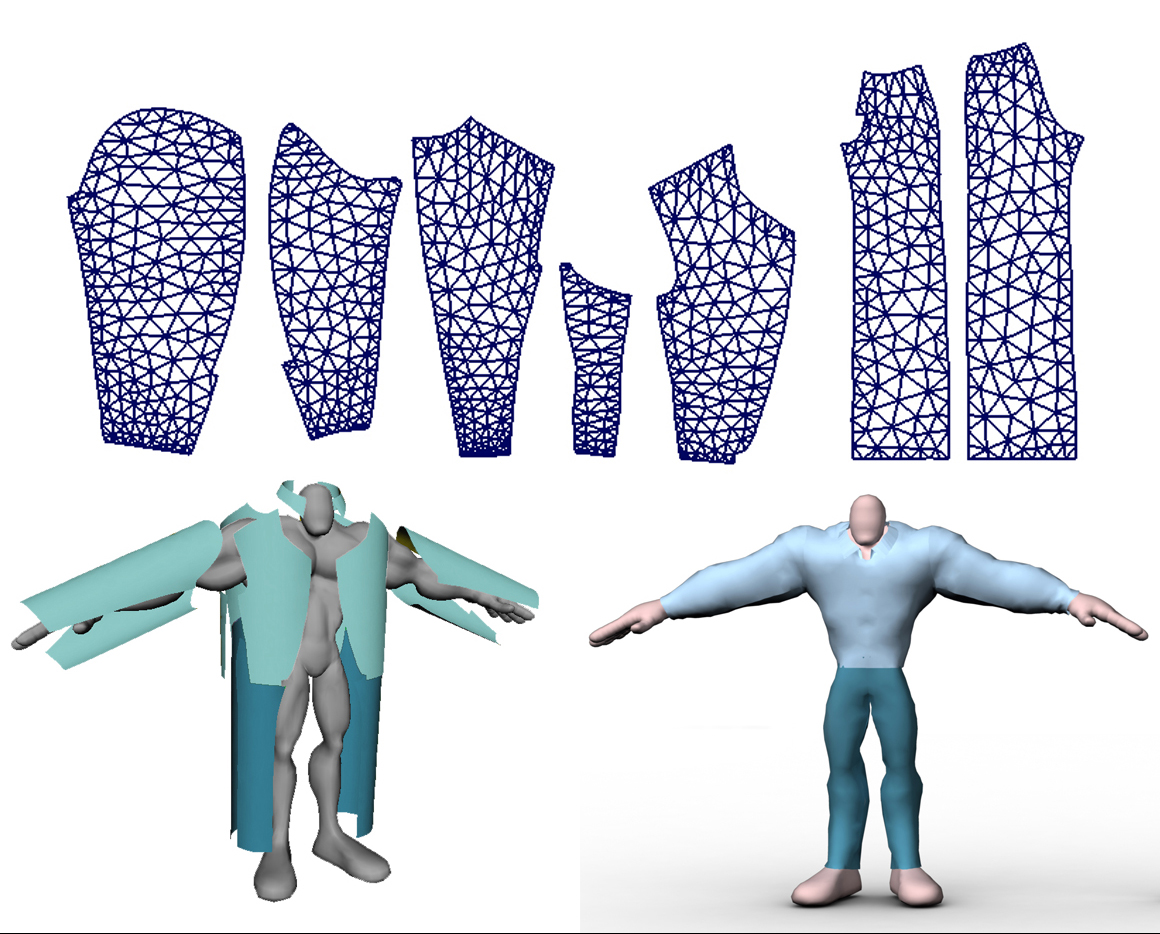
\includegraphics[width=0.9\columnwidth]{../images/resultA}\\
    \caption{Dressing result for character A}
    \label{figure:character_A_pattern}
\end{figure}


\begin{figure}[H]
	\centering
	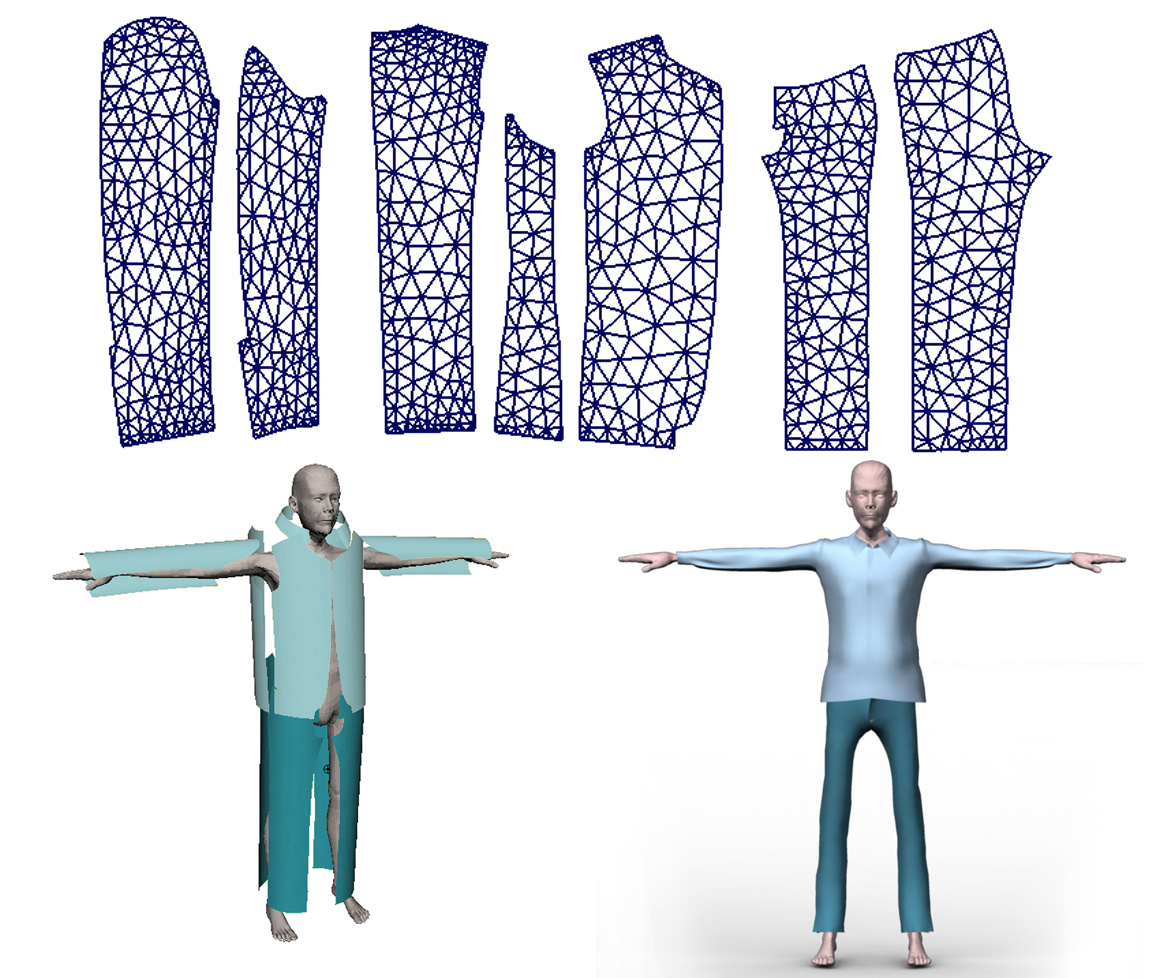
\includegraphics[width=0.9\columnwidth]{../images/resultB}\\
    \caption{Dressing result for character B}
    \label{figure:character_B_pattern}
\end{figure}


\begin{figure}[H]
	\centering
	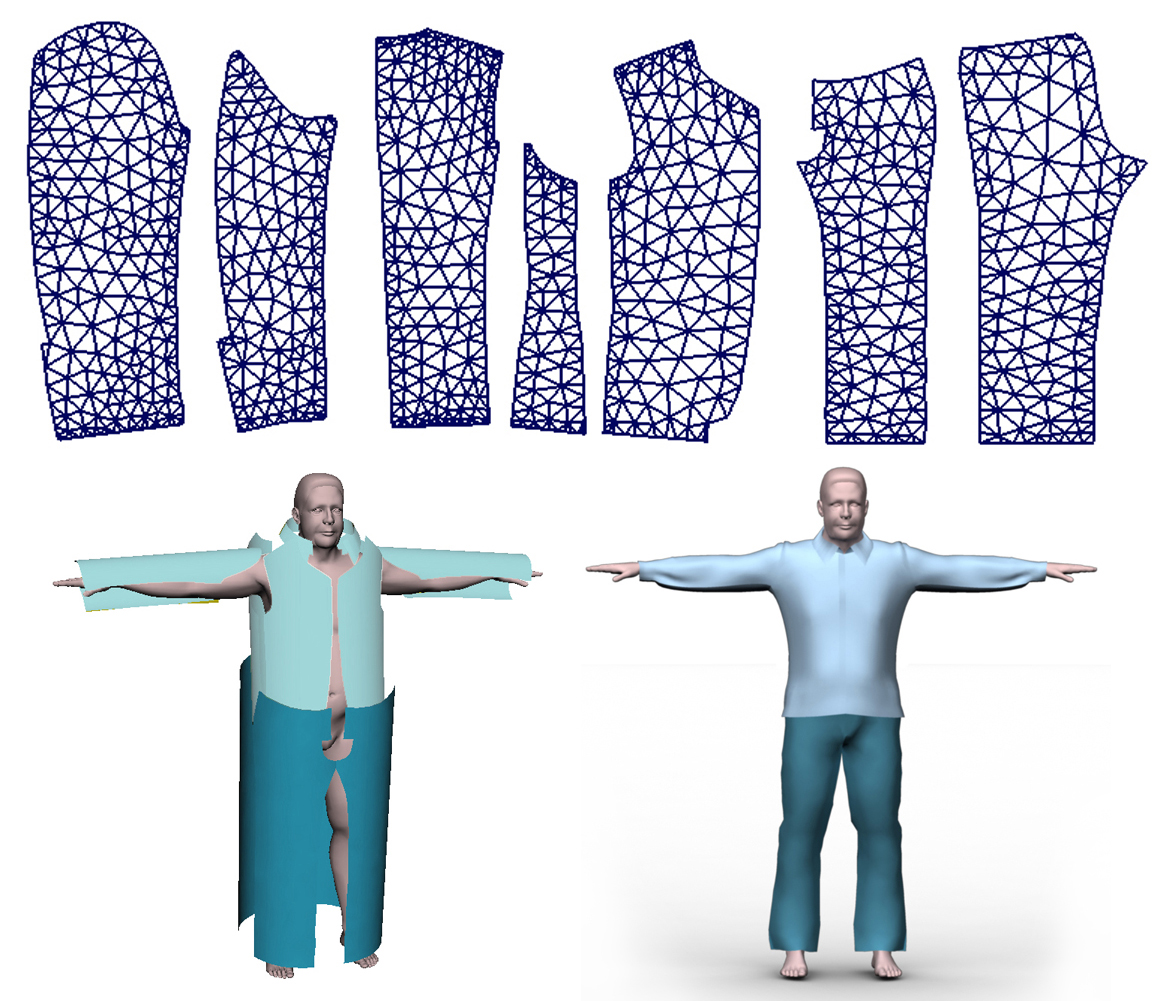
\includegraphics[width=0.9\columnwidth]{../images/resultC}\\
    \caption{Dressing result for character C}
    \label{figure:character_C_pattern}
\end{figure}


\begin{figure}[H]
	\centering
	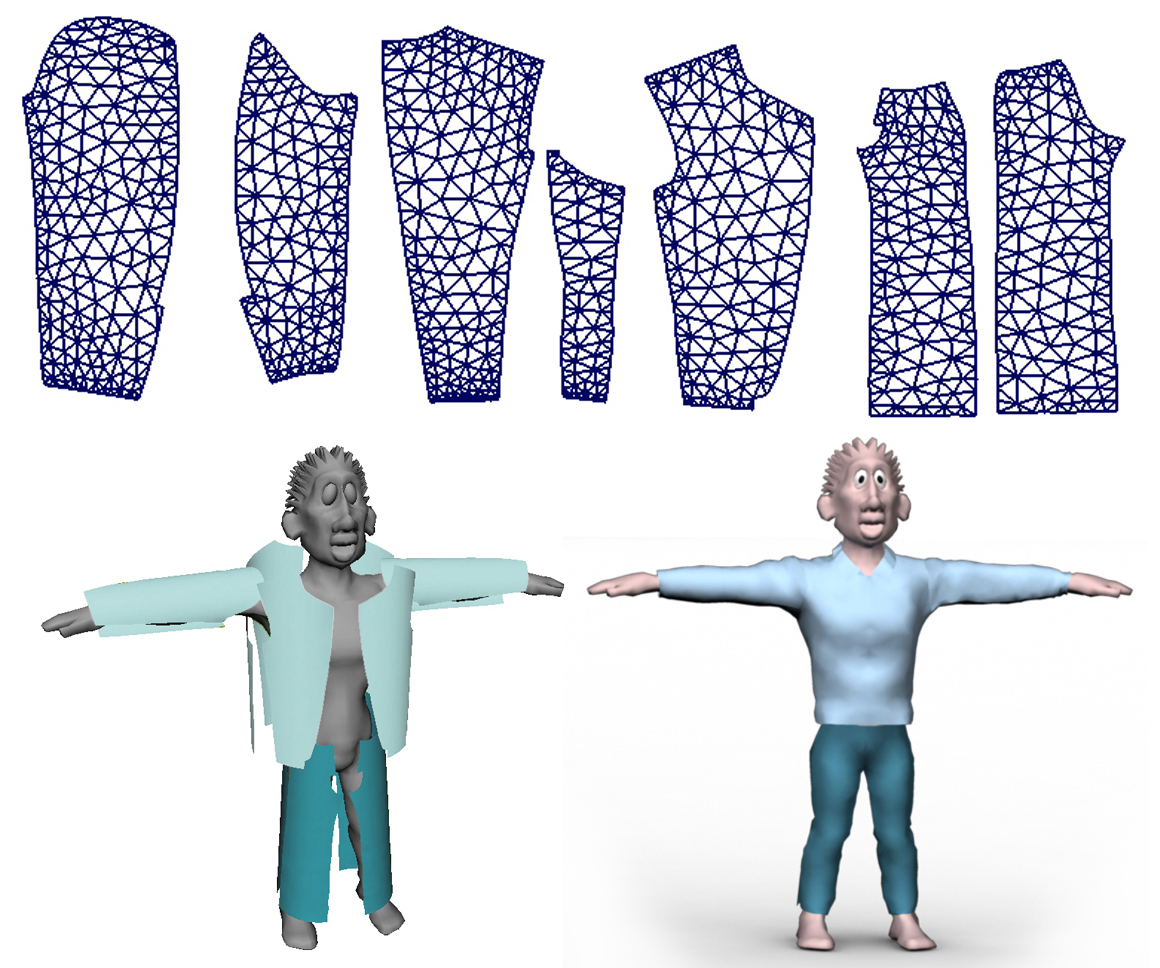
\includegraphics[width=0.9\columnwidth]{../images/resultD}\\
    \caption{Dressing result for character D}
    \label{figure:character_D_pattern}
\end{figure}






%\begin{figure}[H]
%	\centering
%	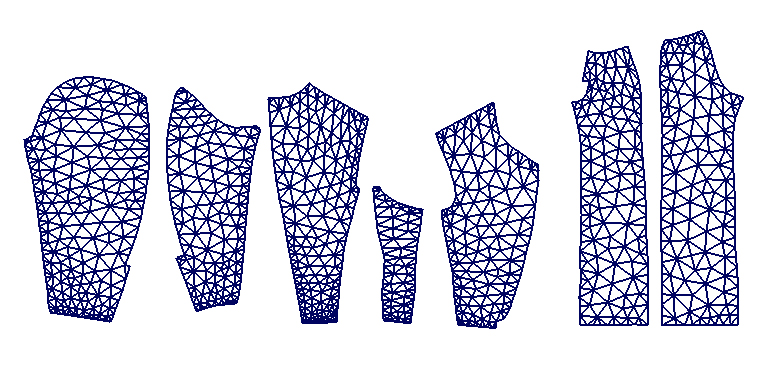
\includegraphics[width=1.0\columnwidth]{../images/hulk_patterns}\\[0.1cm]
%    \caption{Patterns for Character A}
%    \label{figure:character_A_pattern}
%\end{figure}
%
%\begin{figure}[H]
%	\centering
%	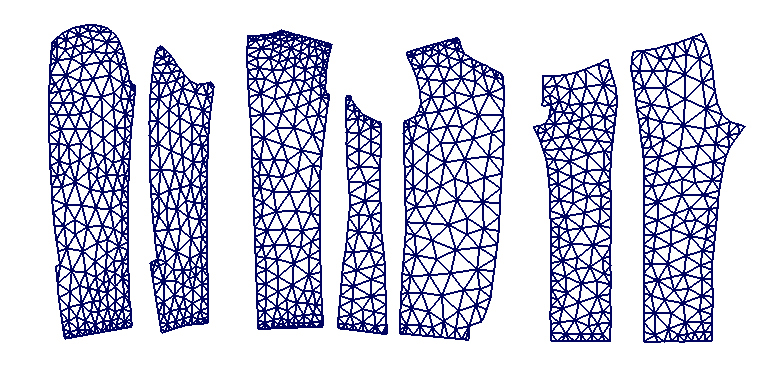
\includegraphics[width=1.0\columnwidth]{../images/skinny_patternsjpg}\\[0.1cm]
%    \caption{Patterns for Character B}
%    \label{figure:character_B_pattern}
%\end{figure}
%
%\begin{figure}[H]
%	\centering
%	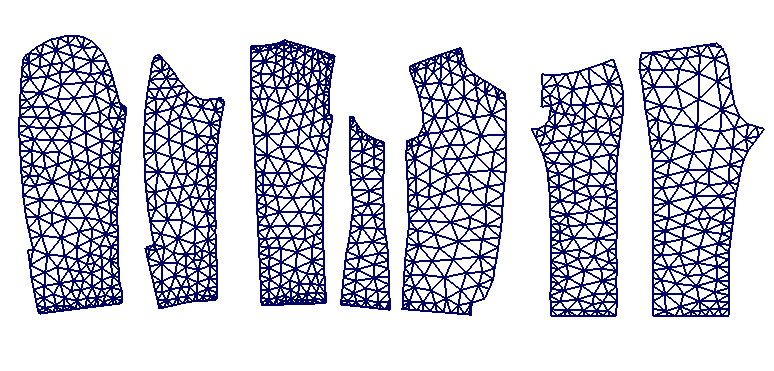
\includegraphics[width=1.0\columnwidth]{../images/fatty_pattern}\\[0.1cm]
%    \caption{Patterns for Character C}
%    \label{figure:character_C_pattern}
%\end{figure}
%
%\begin{figure}[H]
%	\centering
%	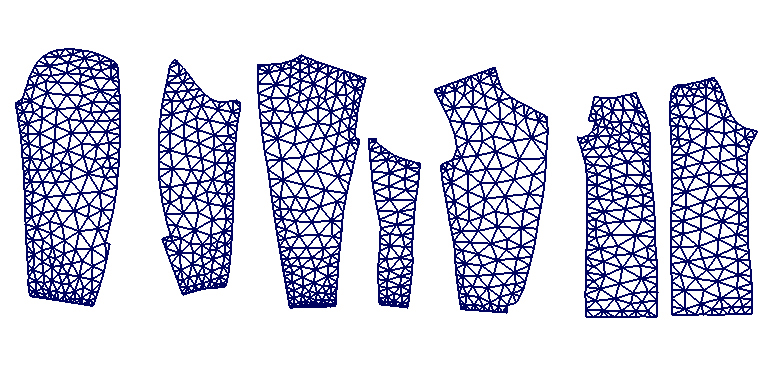
\includegraphics[width=1.0\columnwidth]{../images/shortty_patterns}\\[0.1cm]
%    \caption{Patterns for Character D}
%    \label{figure:character_D_pattern}
%\end{figure}
%
%\begin{figure}
%        \centering
%                
%        \begin{subfigure}[b]{0.5\textwidth}
%                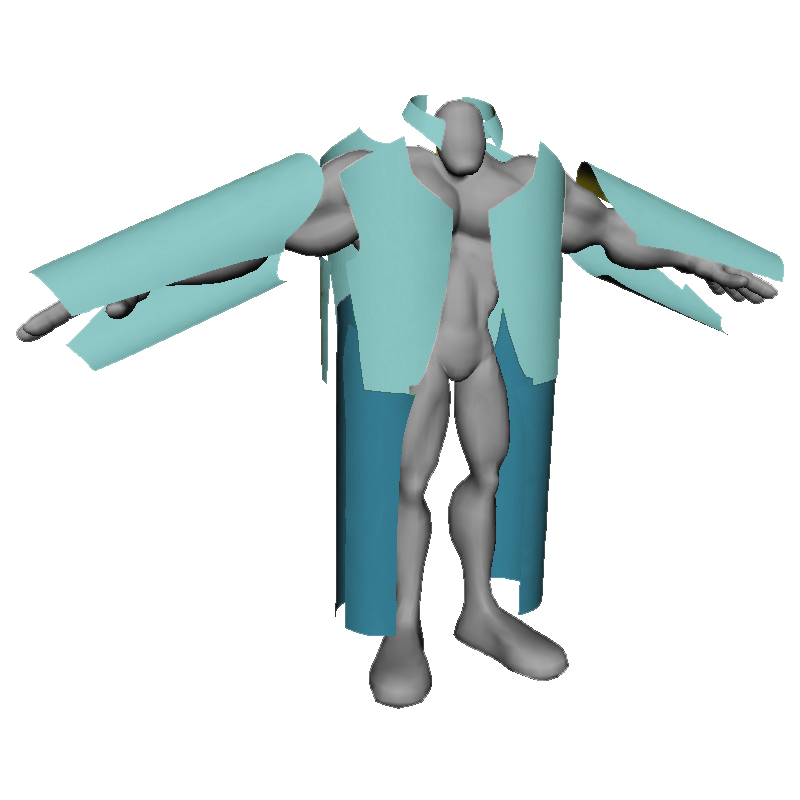
\includegraphics[width=\textwidth]{../images/A_3D_pattern}
%                \caption{Character A}
%                \label{fig:3d_pattern_on_A}
%        \end{subfigure}%
%        ~ %add desired spacing between images, e. g. ~, \quad, \qquad etc.
%          %(or a blank line to force the subfigure onto a new line)
%        \begin{subfigure}[b]{0.5\textwidth}
%                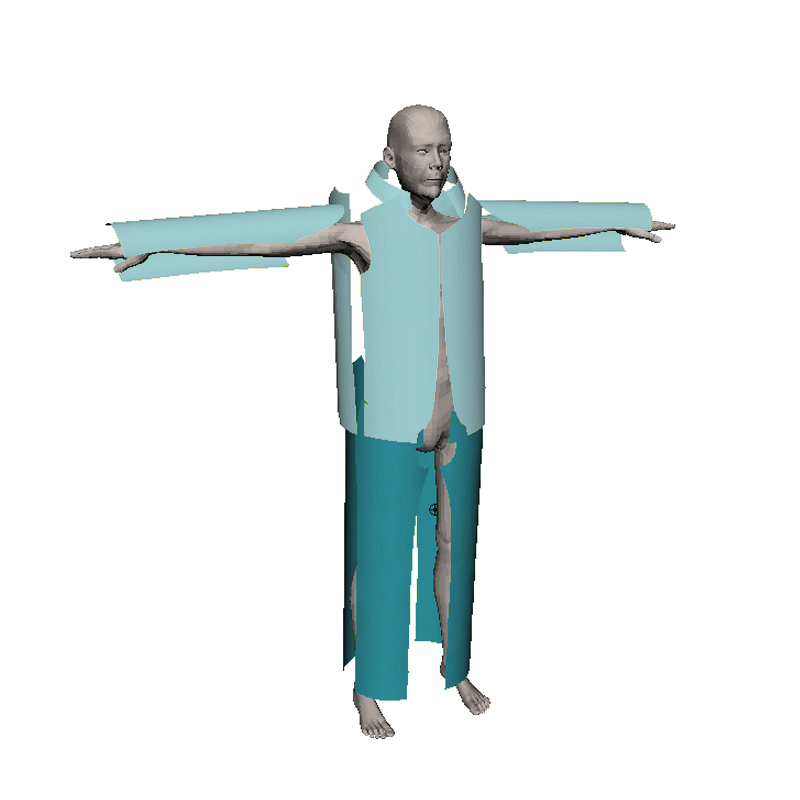
\includegraphics[width=\textwidth]{../images/B_3D_pattern}
%                \caption{Character B}
%                \label{fig:3d_pattern_on_B}
%        \end{subfigure}
%             
%        \begin{subfigure}[b]{0.5\textwidth}
%                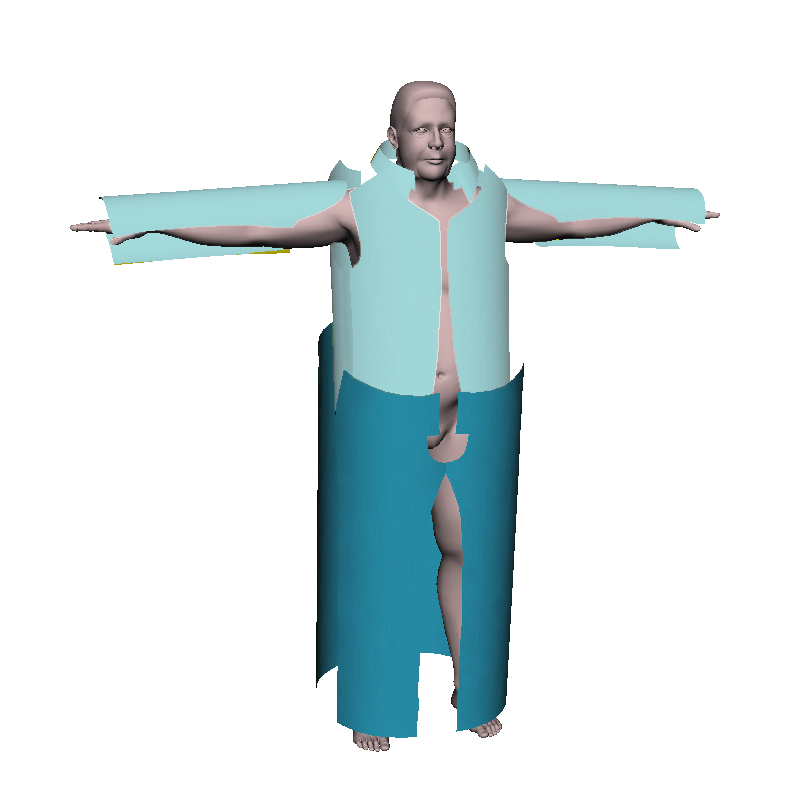
\includegraphics[width=\textwidth]{../images/C_3D_pattern}
%                \caption{Character A}
%                \label{fig:3d_pattern_on_C}
%        \end{subfigure}%
%        ~ %add desired spacing between images, e. g. ~, \quad, \qquad etc.
%          %(or a blank line to force the subfigure onto a new line)
%        \begin{subfigure}[b]{0.5\textwidth}
%                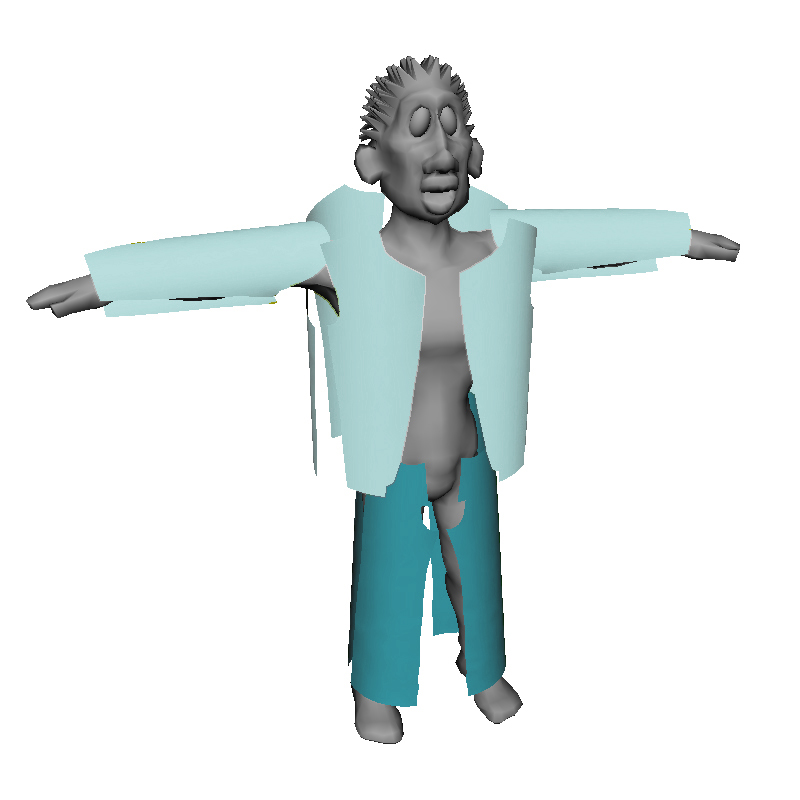
\includegraphics[width=\textwidth]{../images/D_3D_pattern}
%                \caption{Character B}
%                \label{fig:3d_pattern_on_D}
%        \end{subfigure}
%
%        \caption{3D Patterns on the bounding surface of characters}
%        \label{fig:3d_patterns_on_characters}       
%\end{figure}
%\pagebreak

\begin{figure}[H]
	\centering
	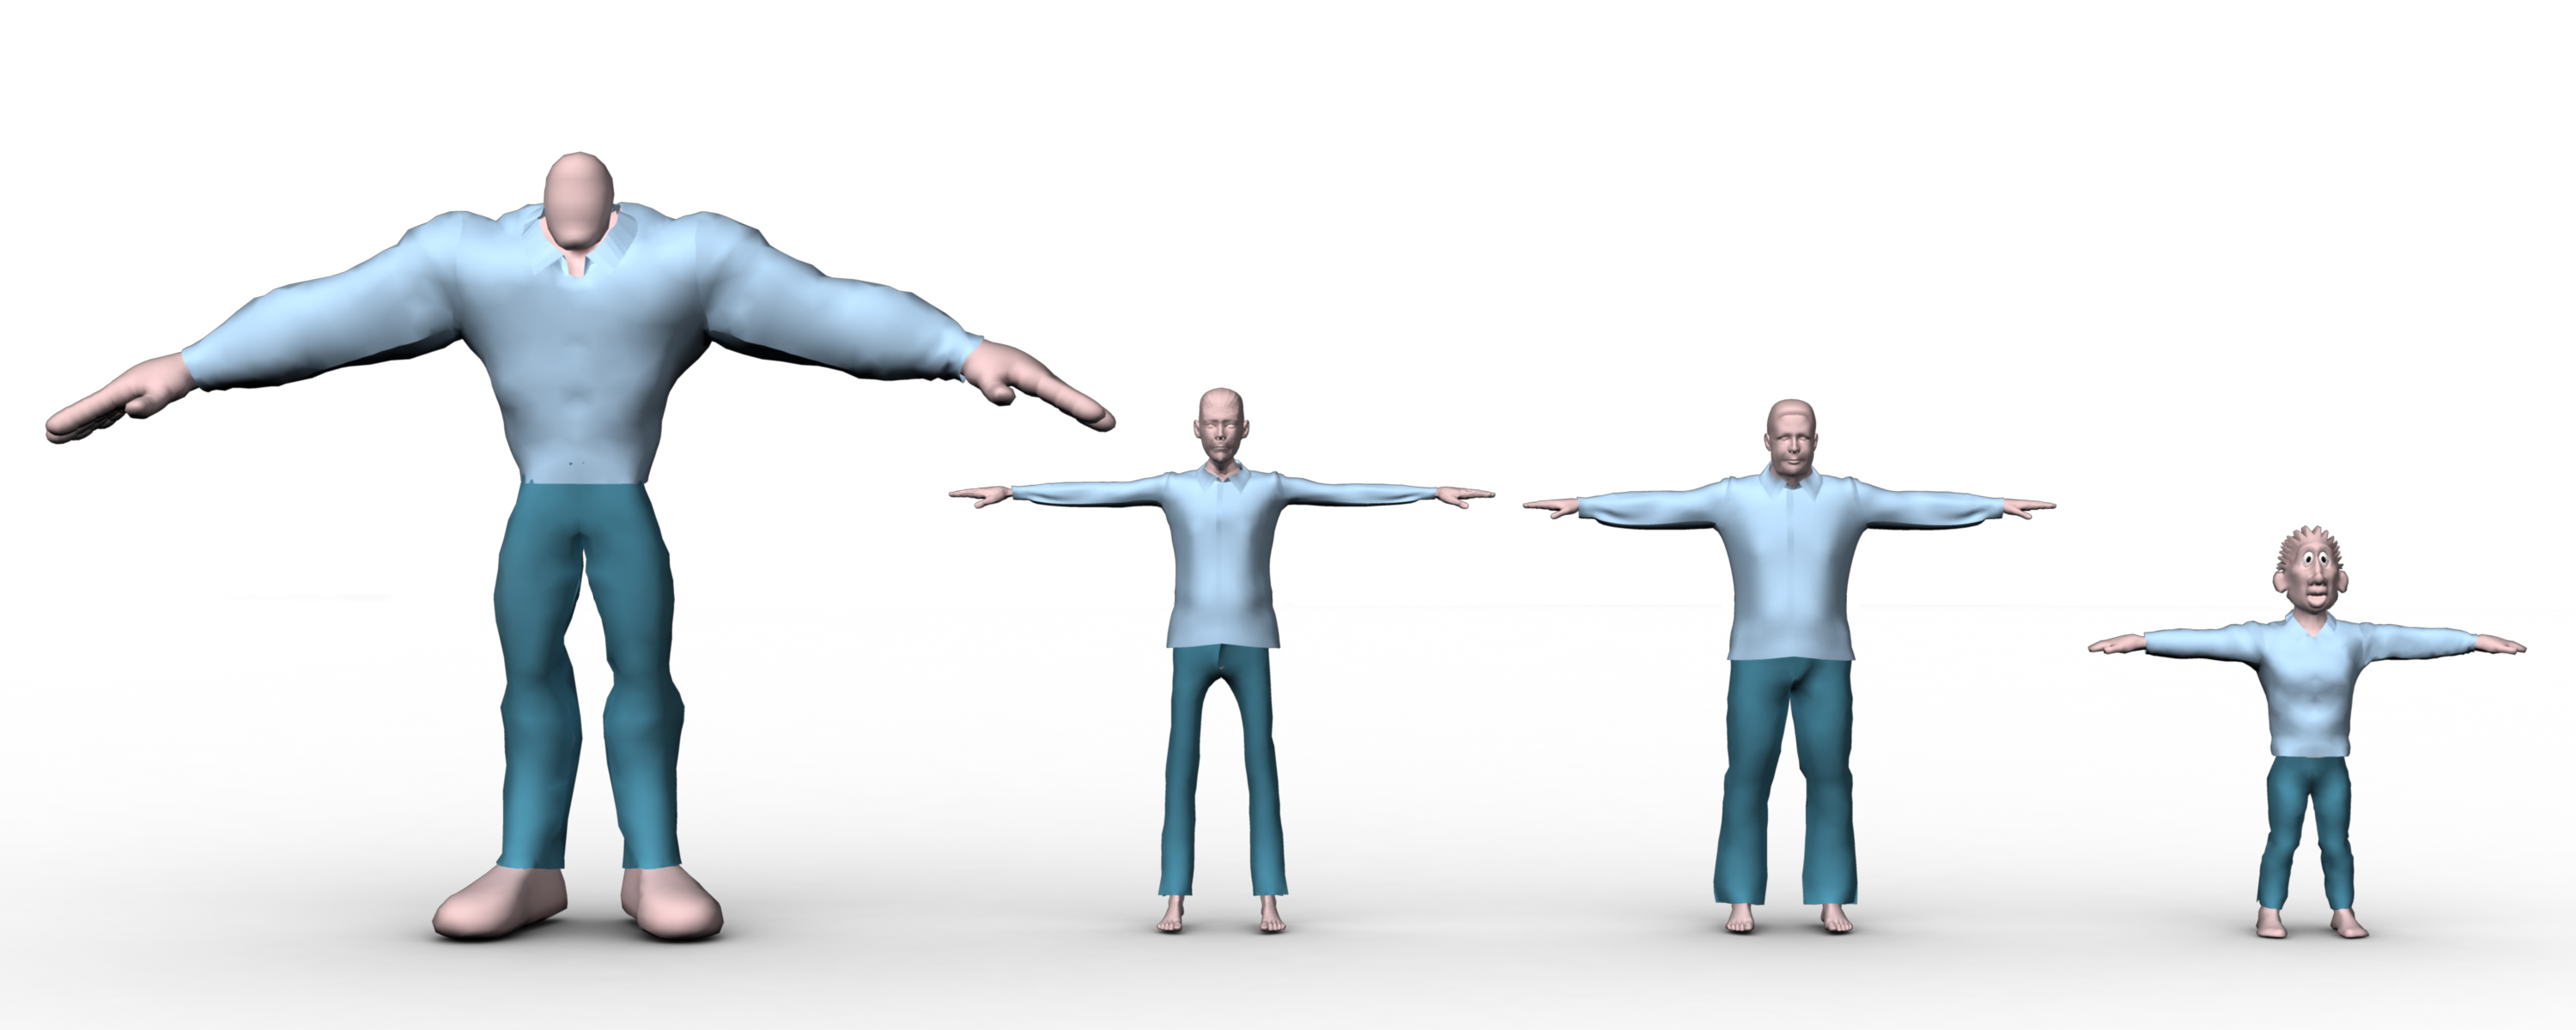
\includegraphics[width=1.0\columnwidth]{../images/all_characters_with_cloth}\\[0.1cm]
    \caption[Front view of dressed up characters]{Front view of four different characters in the same cloth design.}
    \label{figure:final_result_front}
\end{figure}

\begin{figure}[H]
	\centering
	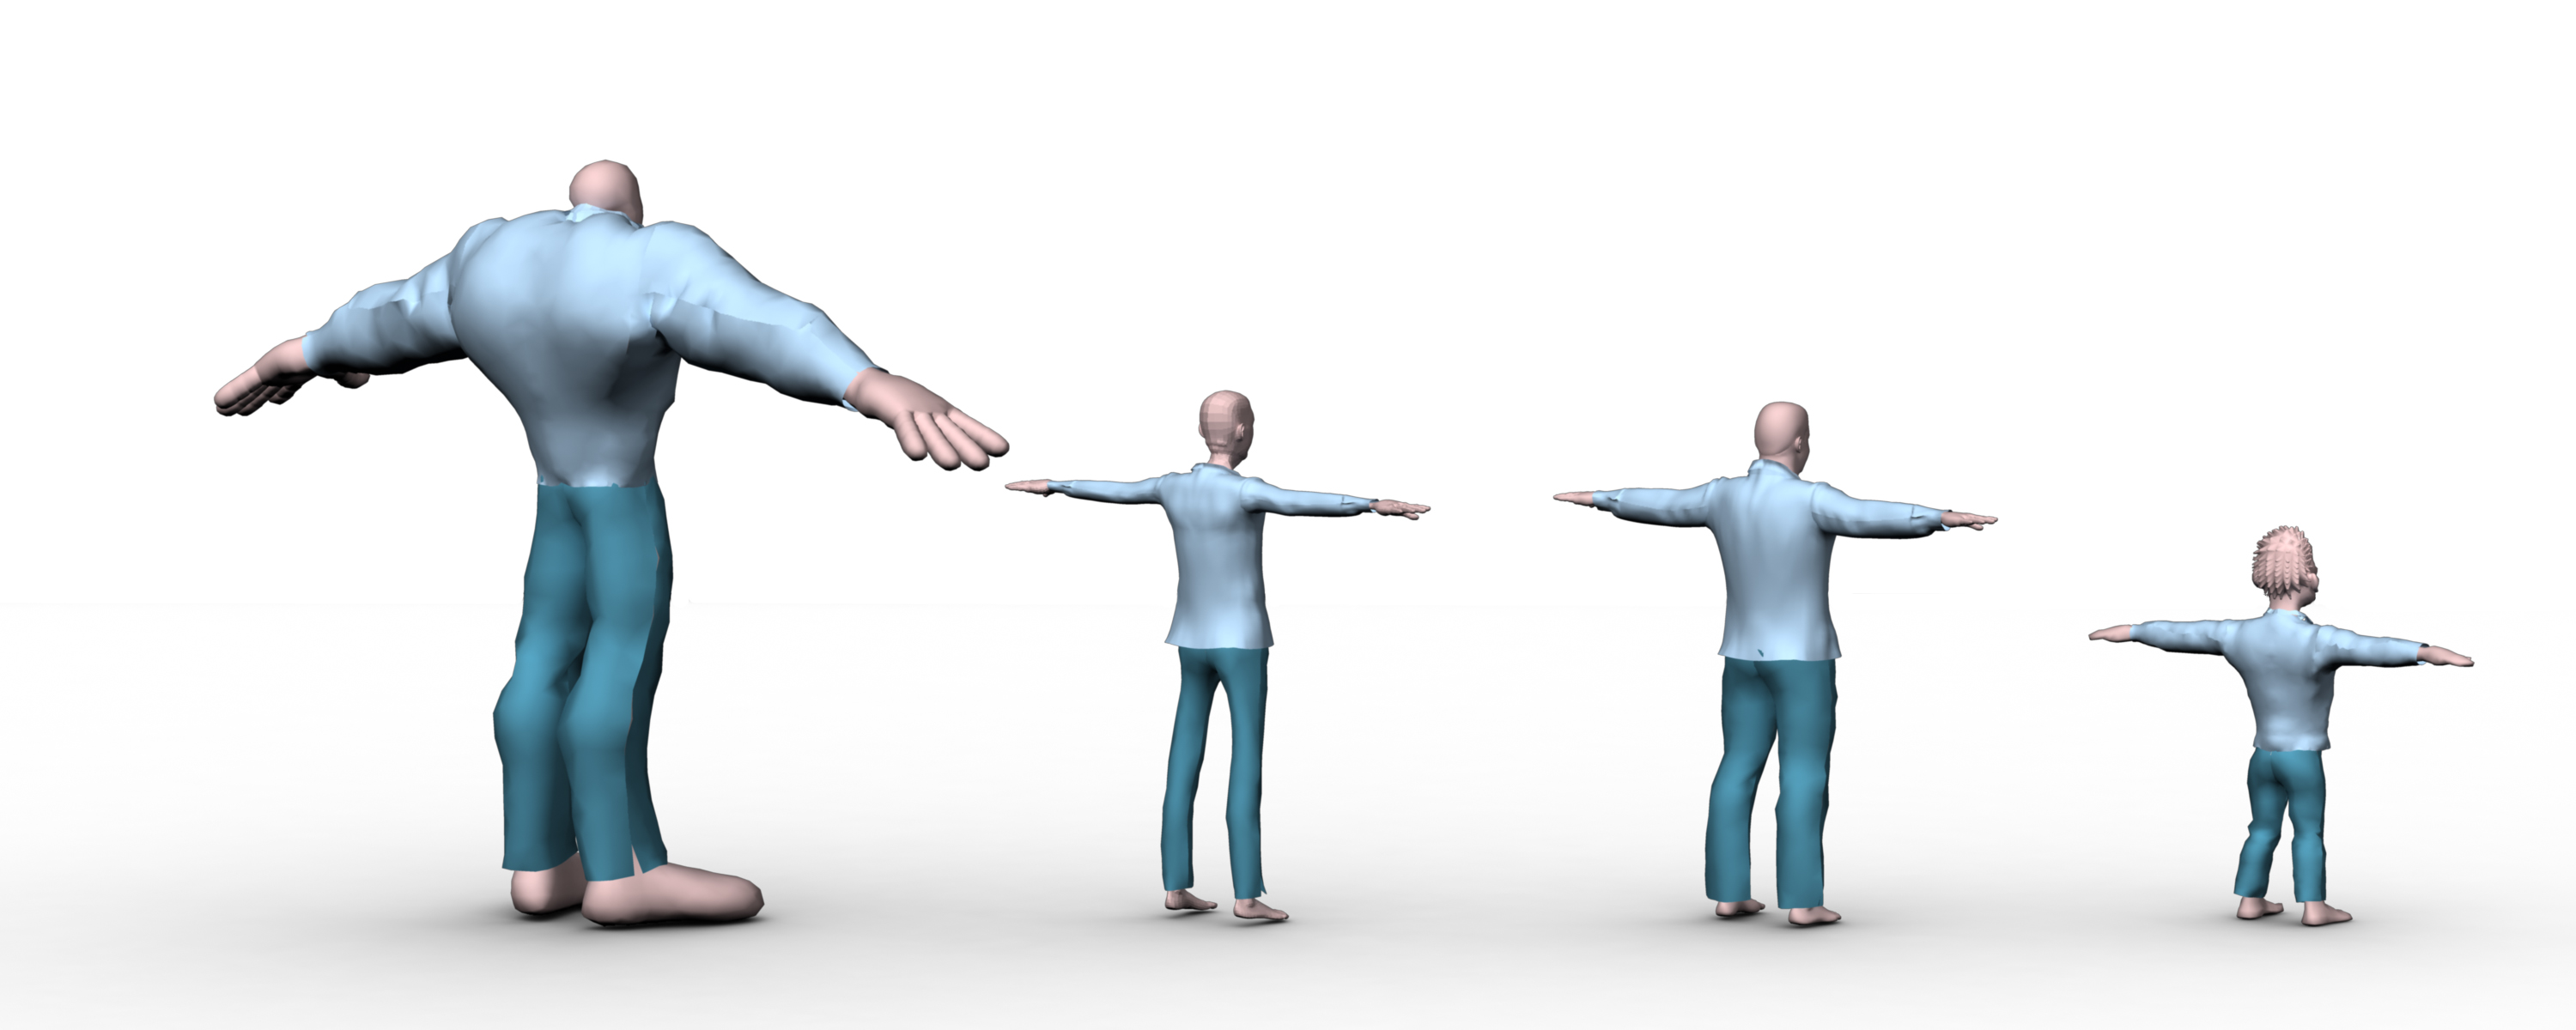
\includegraphics[width=1.0\columnwidth]{../images/all_characters_with_cloth2}\\[0.1cm]
    \caption[Rear view of dressed up characters]{Rear view of four different characters in the same cloth design.}
    \label{figure:final_result_back}
\end{figure}



\begin{table}[H]
    \centering
    \small
    \begin{tabular}{|p{2.2cm}|p{2cm}|p{2cm}|p{2cm}|p{2cm}|}
        \hline
        Evaluation function  & Character A & Character B & Character C & Character D\\
        \hline
        Measurements & 2.927 & 1.803 & 2.125 & 2.842\\
        \hline
        Seamline  & 1.142	&  1.248 &	1.440 & 1.384\\
        \hline
        Shape & 0.446 & 0.112 & 0.092 & 0.389\\
        \hline
        Running time & 784 sec & 791 sec & 752 sec & 743 sec \\
        \hline
    \end{tabular}
    \caption[Fitness values of the final solution]{The fitness values of three evaluation function of the final solution for all characters and the running time for each character, unit of time is second, node that smaller value indicates better fit to the criteria.}
    \label{table:GA_errors}
\end{table}
\setlength{\tabcolsep}{6pt}

In order to further demonstrate the modelling ability of proposed cloth modelling method, three new character is introduced and several types of cloth ranging from female dress to t-shirt are modelled for these characters, the results are demonstrated in Figure \ref{figure:seven_characters_model} to Figure \ref{figure:seven_characters_dress3}. 

\begin{figure}[H]
	\centering
	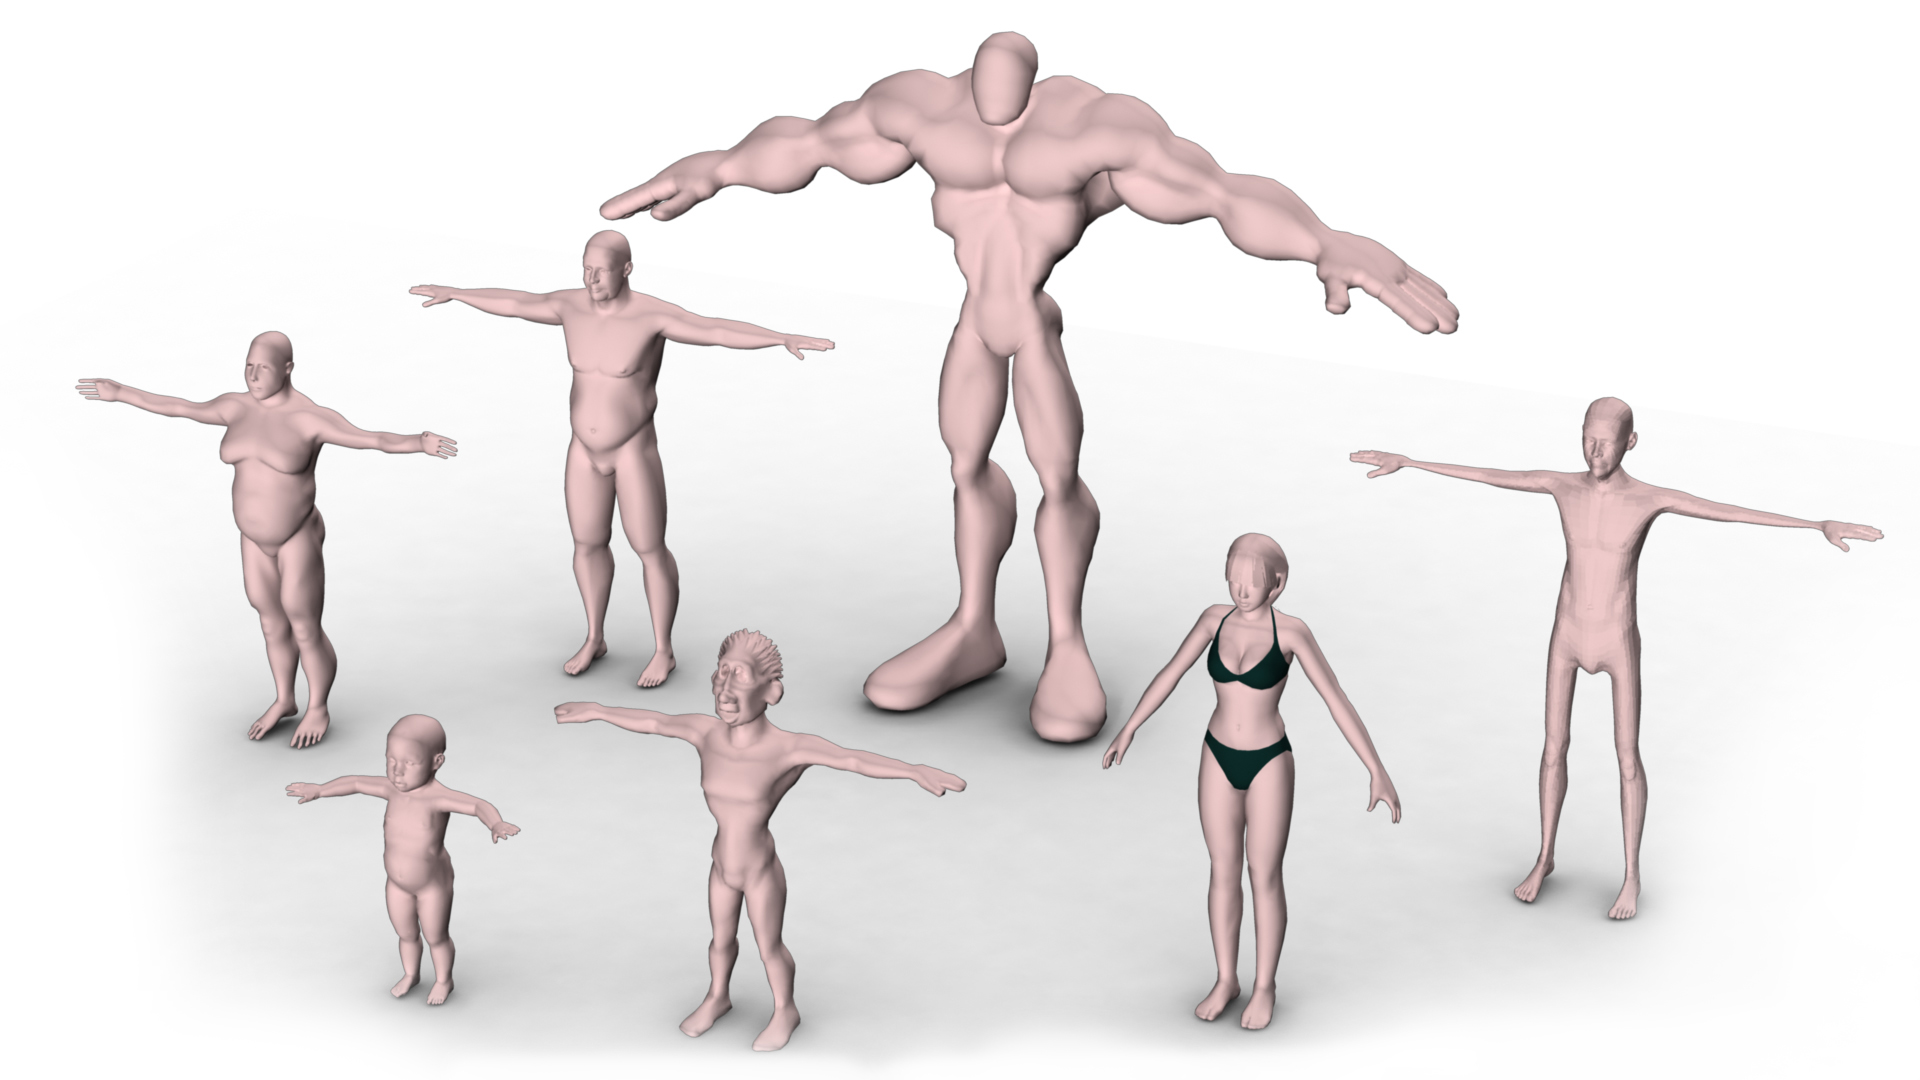
\includegraphics[width=1.0\columnwidth]{../images/7_characters}\\[0.1cm]
    \caption{Characters used for dressing various clothes}
    \label{figure:seven_characters_model}
\end{figure}

\begin{figure}[H]
	\centering
	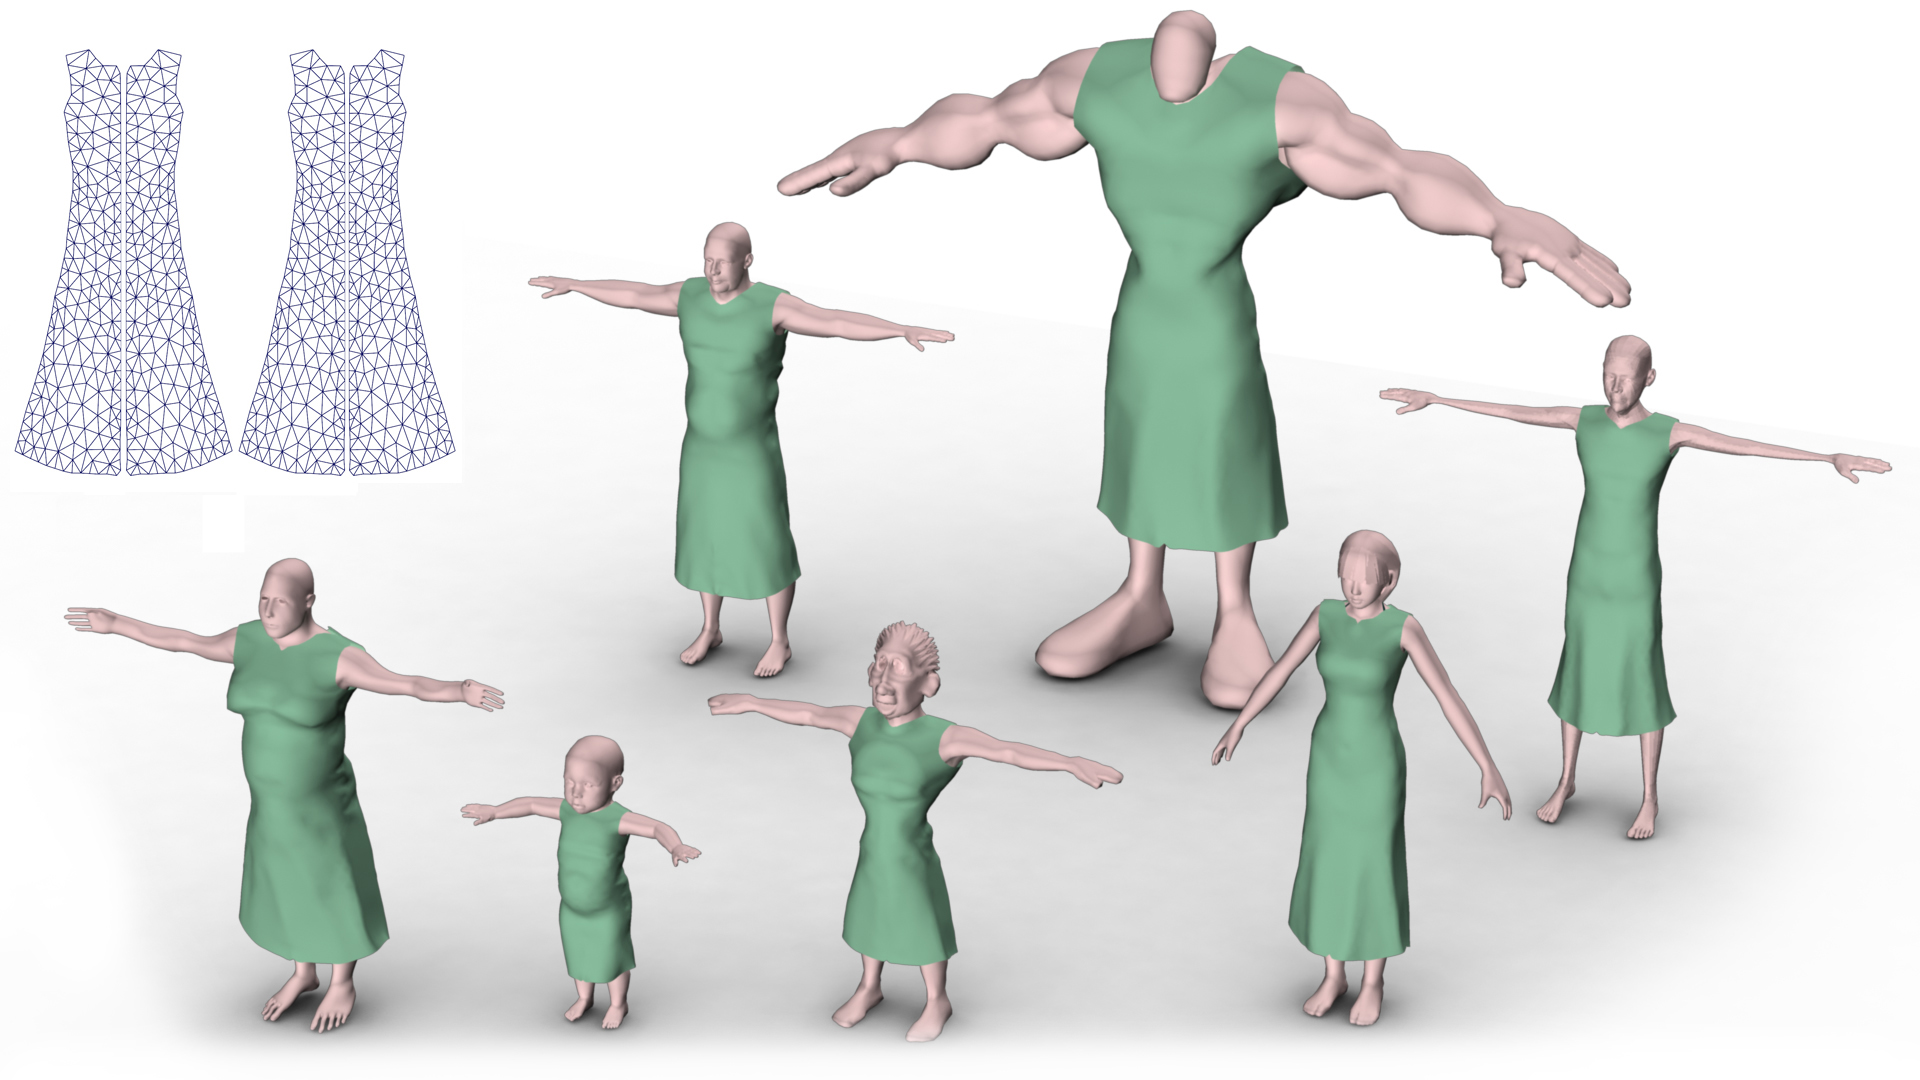
\includegraphics[width=1.0\columnwidth]{../images/7_characters_dress1}\\[0.1cm]
    \caption{Tight dress on different characters}
    \label{figure:seven_characters_dress1}
\end{figure}

\begin{figure}[H]
	\centering
	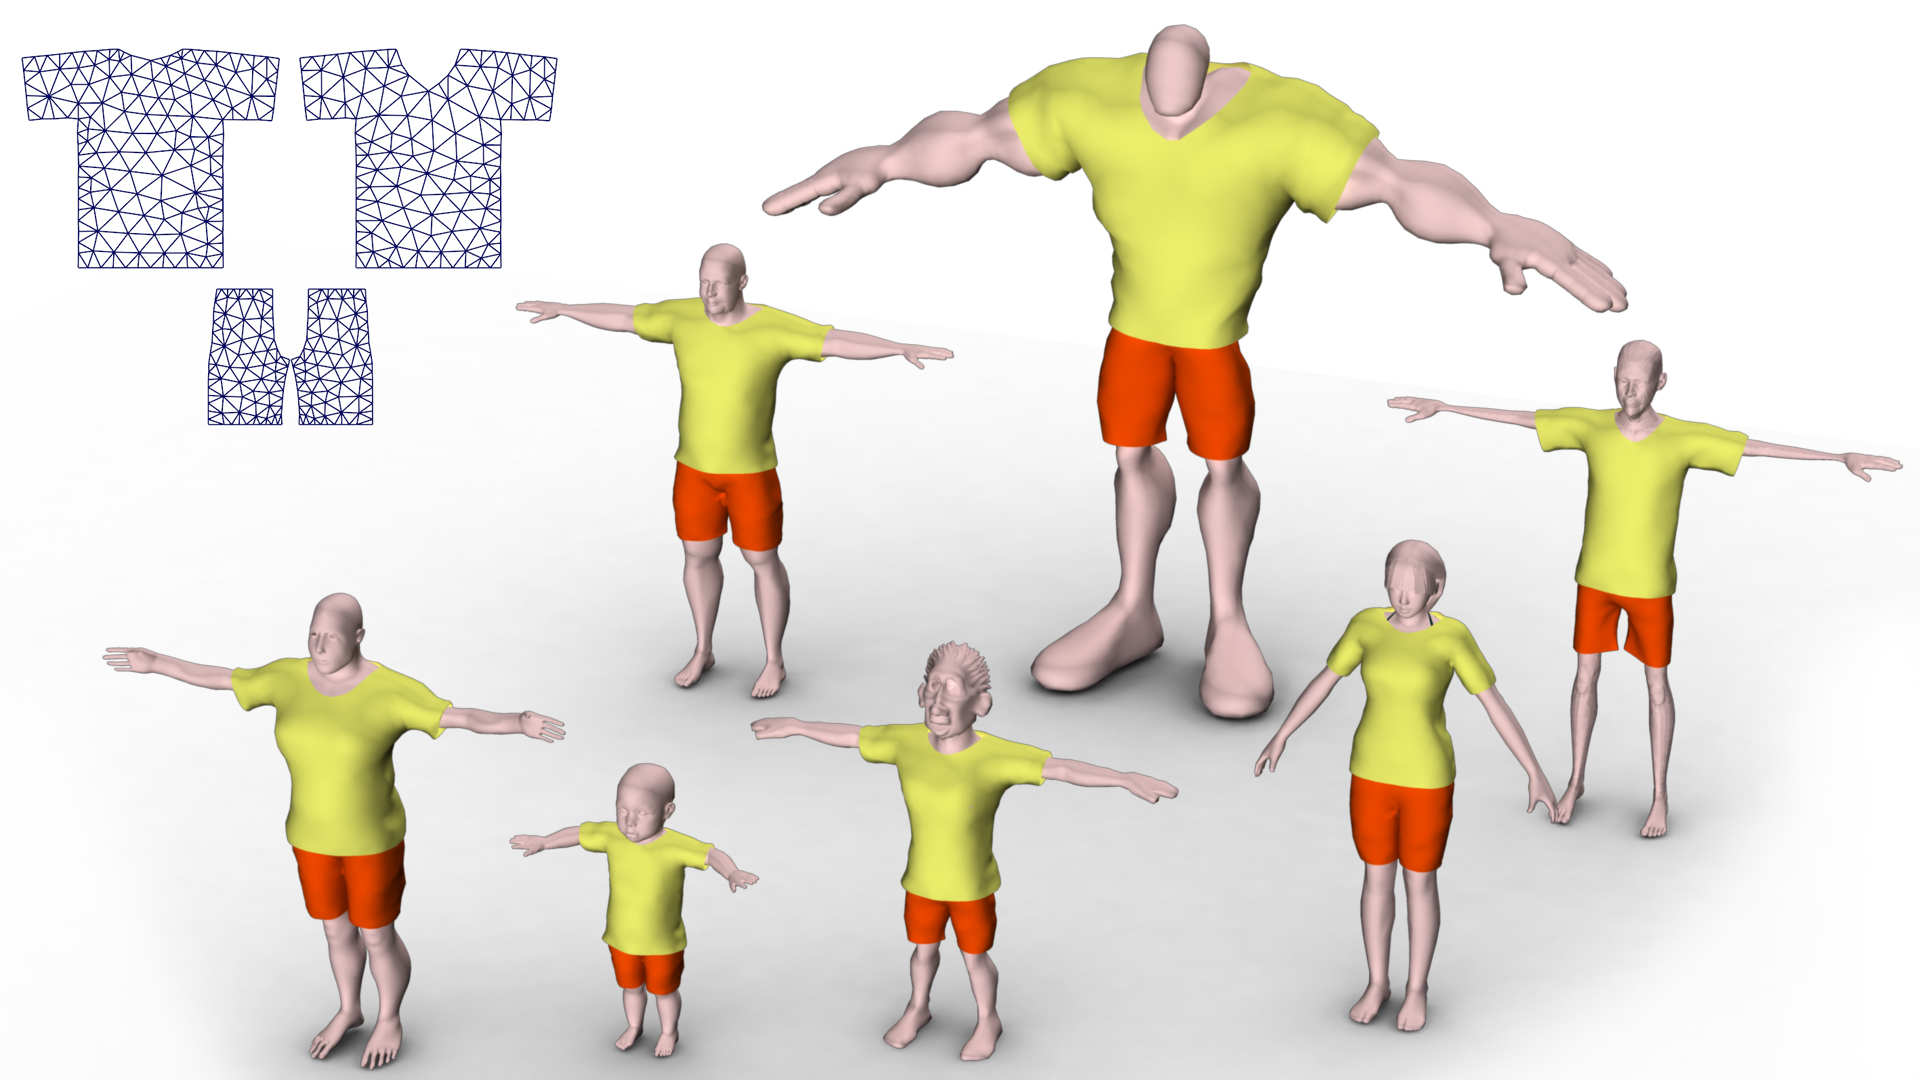
\includegraphics[width=1.0\columnwidth]{../images/7_characters_dress2}\\[0.1cm]
    \caption{T-Shirt and short on different characters}
    \label{figure:seven_characters_dress2}
\end{figure}

\begin{figure}[H]
	\centering
	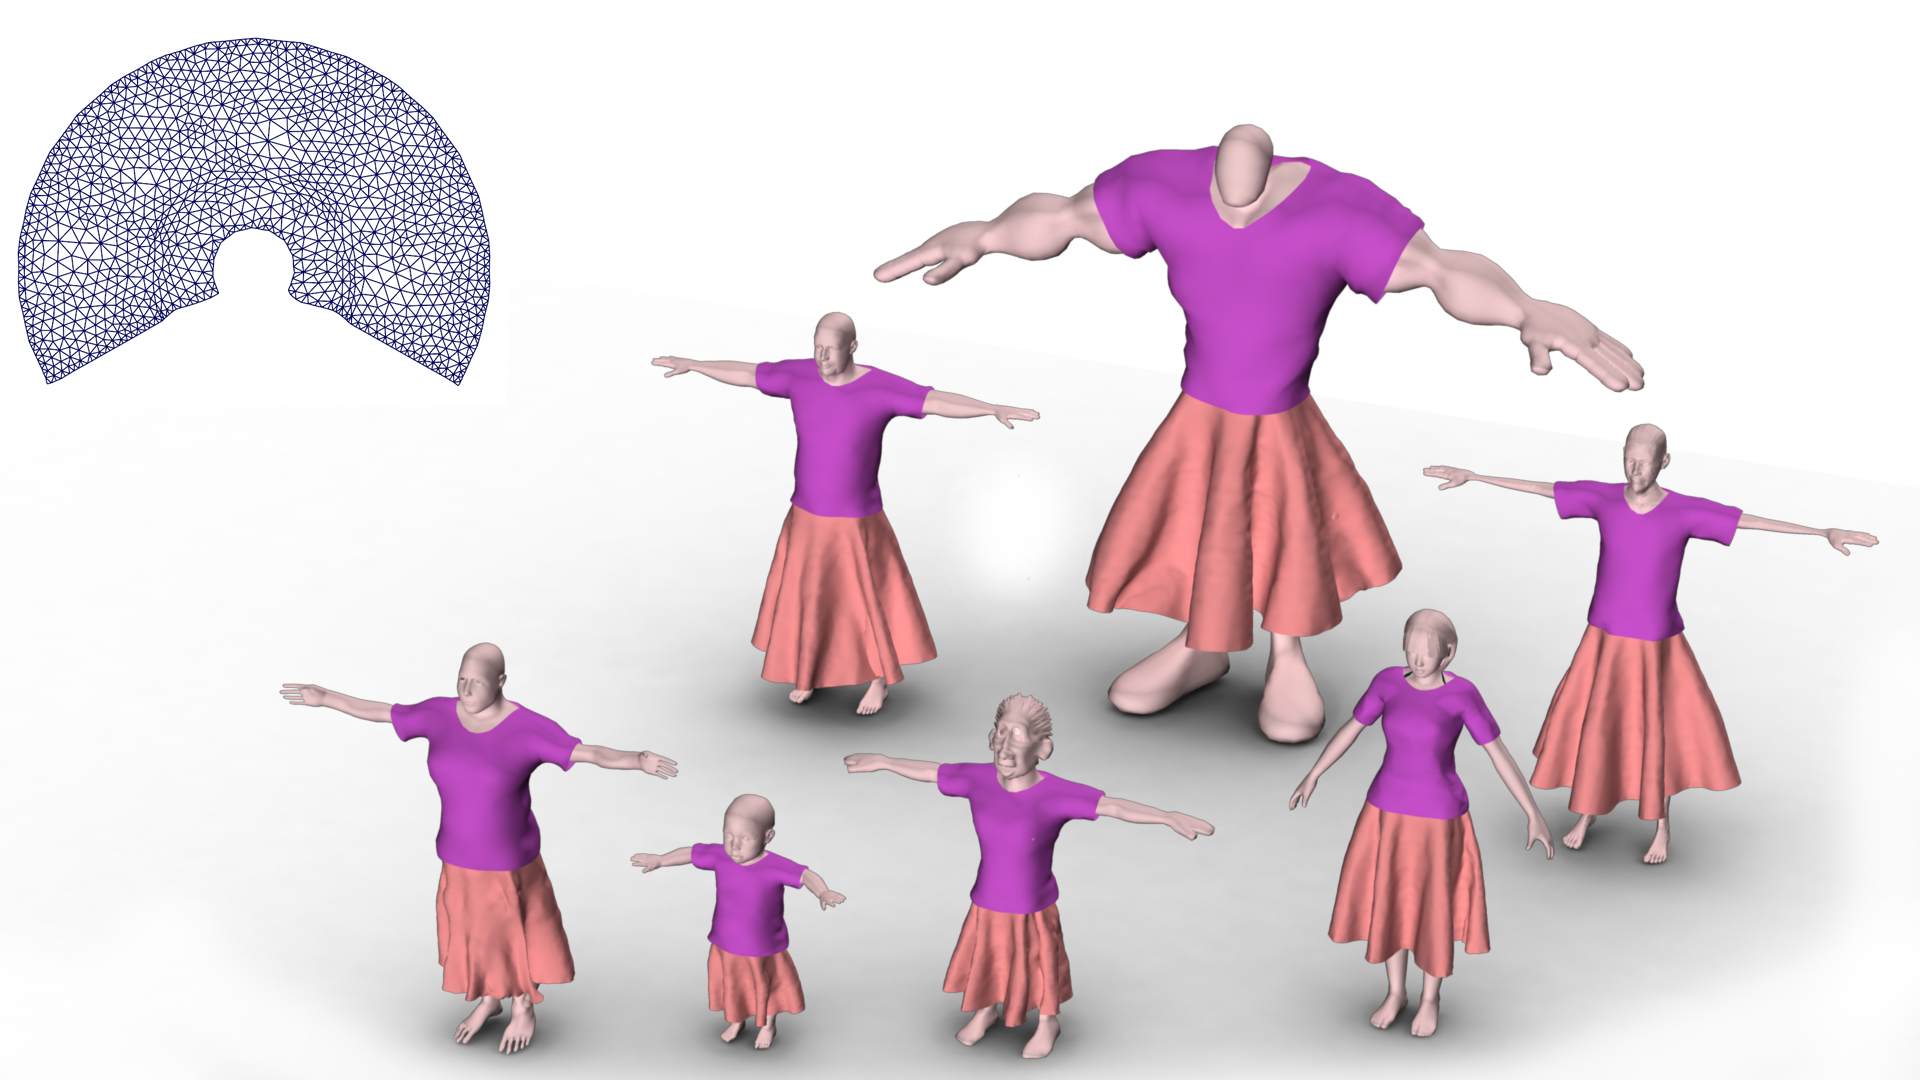
\includegraphics[width=1.0\columnwidth]{../images/7_characters_dress3}\\[0.1cm]
    \caption{Skirt on different characters}
    \label{figure:seven_characters_dress3}
\end{figure}


\section{Conclusions}

This chapter presented an automatic pattern based cloth modelling method for dressing cloth onto characters with different body shapes and proportions. This method takes 2D cloth patterns as inputs. By extracting the measurements from a character model, the shape and size of the cloth patterns are adjusted automatically to fit the cloth onto a character. During pattern adjustment, by considering the measurements, seam-line among the patterns as well as the shape of each pattern, the original design of the cloth is preserved throughout the fitting process. Finally, all patterns are transformed into mesh and positioned around the body, physical simulation is used to stitch all the patterns together based on seam-lines on each pattern to construct the final 3D cloth. 

This method utilises genetic algorithm to adjust cloth patterns for cloth fitting. It has four major advantages. 

Firstly, given the measurements of any character, this method can fits the cloth onto the character automatically. By automating the pattern adjustment process using genetic algorithm, the manual pattern adjustments that required by the current pattern based cloth modelling methods can be avoid. The duplication of effort required by traditional cloth modelling method can be eliminated and the efficiency for modelling cloth for different characters with different body shapes and proportion can be largely improved. This advantages shines itself even more when multiple different characters are required in the virtual environment. 

Secondly, this method models cloth based on cloth design patterns without requiring tailoring expertise. By automating pattern adjustment process, deep tailoring knowledge involved in patternmaking process can be avoided. This method provides an efficient and easy-to-use solution for the  animation artists. It empowers their creativity and improves their productivity by allowing them to use the large amount of existing cloth patterns in the fashion industry to create various clothes that fit different characters. 

Thirdly, this method generates 3D cloth based on the adjusted 2D cloth patterns. The cloth modelling workflow is proceed in one direction. There is no turning back for extracting patterns from 3D cloth which is required by current cloth modelling method.
Therefore, the shape distortion that is introduced by 3D surface flattening process can be avoid and the extra computation for 2D pattern extracting can also be eliminated. 

Most importantly, cloth are represented by 2D pattern initially, which is the unified form for all clothes. A modelled cloth can be stored in asset warehouse in the form of cloth pattern. When dressing a new character, only measurements of that character need to be recalculated and existing cloth pattern can be reused to fit a cloth onto the new character automatically. The reusability of modelled cloth is improved significantly by modelling cloth from patterns. 


%However, many method that developed for dressing character are operator directly on 3D cloth object such as \Citet{brouet:hal-00695903}. Directly manipulating vertex on 3D cloth mesh to achieve fit is able to produce compelling result. However, the propose of garment pattern previewing is to create the 3D visual preview of 2D patterns. If a cloth is resized in 3D space, all the pattern need to be remapped from 3D space onto 2D planer in order to produce the pattern for resized cloth. However, the patten in 3D space is hardly maintain developable surface ones its vertex is modified. Therefore, the mapping operation from fitted 3D cloth object to 2D pattern  can introduce error into the resized cloth pattern. In the method that presented in this chapter, all the resizing are done in 2D pattern before the sewing, therefore, the cloth that formed onto 3D subject is the ``actual'' preview of the pattern design. This feature avoid the introduction of errors when mapping an undevelopable mesh onto a 2D planner. 
%
%This method combines the traditional clothes making techniques with modern computer graphic techniques to model the cloth from the measurements of the virtual character. 


%**************************************************************************
%**************************************************************************


\ifx\isEmbedded\undefined
% References
\addcontentsline{toc}{chapter}{References}
\bibliographystyle{../ref/harvard}
\bibliography{../ref/phd_references}
\pagebreak
\end{document}
\fi
